\documentclass[12pt]{thesis}


\usepackage{tocloft}
\renewcommand{\cftchapfont}{\bfseries}
\renewcommand{\cftchappagefont}{\bfseries}
\renewcommand{\cftchappresnum}{Chapter }
\renewcommand{\cftchapaftersnum}{:}
\renewcommand{\cftchapnumwidth}{6em}


%some packages may not be needed depending on your use
\usepackage{titlesec}
   \titleformat{\chapter}
      {\normalfont\large}{Chapter \thechapter:}{1em}{}



\usepackage{lipsum} %Remove before final draft, used to generate filler text

\usepackage{cite}
\usepackage{pdflscape} %allows turning pages to landscape
\usepackage{indentfirst}
\usepackage{latexsym}
\usepackage{multirow}
\usepackage{enumerate}
\usepackage{tabls}
\usepackage{wrapfig}%for wrapping text around figures in the document; don't need figure wrapping in this document
\usepackage{longtable}
\usepackage{array}
\usepackage{supertabular}%for large tables that do not fit on a single page; also probably won't need this
%\usepackage{subeqn} %removed to fix error with glossaries package
% \usepackage{subfigure}%allows creation of subfigures (i.e.  Fig #a, Fig. #b...)
\usepackage{microtype}%readablity enhancements
\usepackage[bookmarks, bookmarksnumbered, colorlinks=true, plainpages=false, pdfpagelabels, citecolor=blue, urlcolor=blue, filecolor=blue, linkcolor=blue]{hyperref}
\usepackage{bookmark}%manually add missing bookmarks with \pdfbookmark
\usepackage[toc, nonumberlist]{glossaries} %needs to be after hyperref
\usepackage{amssymb,amsmath,amsfonts,mathrsfs,mathtools,amsthm,bm}
\usepackage{shuffle}
\usepackage{tikz}
\usepackage{pgfplots} % drawing axis, addplots
\pgfplotsset{compat=newest} % ensure position and scaling compatibility
\usetikzlibrary{intersections} % intersections in tikz
\usetikzlibrary{calc} % calculations in tikz, and calculate length of texts
\usetikzlibrary{hobby} % smoothly connecting points
\usetikzlibrary{decorations.markings} % put arrow in the middle
\tikzset{
    ->-/.style={decoration={markings,mark=at position #1 with {\arrow{>}}},postaction={decorate}}
} % use as [->-=#1], put the arrow at #1, where 0 <= #1 <= 1
\usetikzlibrary{arrows}
\tikzset{leftrightsquig/.style={to-to, decorate, decoration={
    zigzag,
    segment length=5,
    amplitude=1,
    pre=lineto,
    post=lineto,
    post length=2pt,
    pre length=2pt}}}
\usepackage{tikz-3dplot}
\usepackage{tikz-cd}

\theoremstyle{definition}
\newtheorem{theorem}{Theorem}[section]
\newtheorem{definition}[theorem]{Definition}
\newtheorem{corollary}[theorem]{Corollary}
\newtheorem{lemma}[theorem]{Lemma}
\newtheorem{proposition}[theorem]{Proposition}
\newtheorem{example}[theorem]{Example}
\newtheorem{problem}[theorem]{Problem}
\newtheorem{conjecture}[theorem]{Conjecture}
\newtheorem{fact}[theorem]{Fact}
\newtheorem{question}[theorem]{Question}
\newtheorem{remark}[theorem]{Remark}

\newtheorem*{theorem*}{Theorem}

% \theoremstyle{remark}
% \newtheorem*{remark}{remark}

\DeclareMathOperator{\INV}{INV}
\DeclareMathOperator{\Li}{Li}
\DeclareMathOperator{\id}{id}
\DeclareMathOperator{\ev}{ev}
\DeclareMathOperator{\Symb}{Symb}
\DeclareMathOperator{\Spec}{Spec}
\DeclareMathOperator{\dep}{dep}
\DeclareMathOperator{\Ext}{Ext}
\DeclareMathOperator{\Aut}{Aut}
\DeclareMathOperator{\Hom}{Hom}
\DeclareMathOperator{\Gr}{Gr}
\DeclareMathOperator{\End}{End}
\DeclareMathOperator{\Lie}{Lie}
\DeclareMathOperator{\gr}{gr}
\DeclareMathOperator{\SL}{SL}

\usepackage{graphicx}
\usepackage{subcaption}
\usepackage{float}
\usepackage{xcolor}
% Cleveref MUST come after ams packages if AMS packages are used.
\usepackage{cleveref}

%Labelling and referencing with section numbers
\numberwithin{equation}{section}
\numberwithin{figure}{section}

% Default value of number of columns in a matrix
\setcounter{MaxMatrixCols}{100}

\newcommand{\tbsp}{\rule{0pt}{18pt}} %used to get a vertical distance after \hline
\renewcommand{\baselinestretch}{2}
\setlength{\textwidth}{5.9in}
\setlength{\textheight}{9in}
\setlength{\topmargin}{-.50in}
\setlength{\oddsidemargin}{.55in}
\setlength{\parindent}{.4in}
\pagestyle{empty}


\setacronymstyle{long-short} %first use of acronym gives full name
\glsdisablehyper %turns off hyperlinking
% \loadglsentries{definitions} %defines file with all entries
\renewcommand{\glossarysection}[2][]{} %Hides glossary title so it can be named manually
\makeglossaries


\begin{document}
\hypersetup{pageanchor=false} %Fixes hyperref error with unnumbered title pages
% !TEX root = ../mainthesis.tex

%Abstract Page
\pdfbookmark{Abstract}{abstract}
\hbox{\ }

\renewcommand{\baselinestretch}{1}
\small \normalsize

\begin{center}
\large{{ABSTRACT}}

\vspace{3em}

\end{center}
\hspace{-.15in}
\begin{tabular}{ll}
Title of dissertation:
&{\large HOPF ALGEBRA OF MULTIPLE}\\
&{\large POLYLOGARITHMS AND ASSOCIATED}\\
&{\large MIXED HODGE STRUCTURES}\\
\ \\
&{\large Haoran Li}\\
&{\large Doctor of Philosophy, 2024} \\
\ \\
Dissertation directed by:
&{\large Professor Christian Zickert} \\
&{\large Department of Mathematics} \\
\end{tabular}

\vspace{3em}

\renewcommand{\baselinestretch}{2}
\large \normalsize

This thesis constructs a variation of mixed Hodge structures based on multiple polylogarithms, and attempts to build candidate complexes for computing motivic cohomology.

Firstly, we consider Hopf algebras with generators representing multiple polylogarithms. By quotienting products and functional relations, we get Lie coalgebras whose Chevalley-Eilenberg complexes are conjectured to compute rational and integral motivic cohomologies. We also associate one-forms to multiple polylogarithms, which exhibit combinatorial properties that are easy to work with. This is joint work with Greenberg, Kaufman and Zickert, which constitues~\cite{ZDHZ_TheLieCoalgebraOfMultiplePolylogarithms} and part of~\cite{ZDHZ_HopfAlgebrasOfMultiplePolylogarithmsAndHolomorphicOneForms}.

Next, we introduce a variation matrix which describes a variation of mixed Hodge structures encoded by multiple polylogarithms. Its corresponding connection form is composed of the one-forms associated to the multiple polylogarithms. This joint work constitutes the remaining part of~\cite{ZDHZ_HopfAlgebrasOfMultiplePolylogarithmsAndHolomorphicOneForms}.

Lastly, to ensure the well-definedness of the Hodge structures, we must compute the monodromies of multiple polylogarithms, for which we provide an explicit formula, extending the previous work done for multiple logarithms, a subfamily of multiple polylogarithms. %(must be first, required, non-numbered)
% !TEX root = ../mainthesis.tex

%Titlepage
\pdfbookmark{Title Page}{titlepage}
\thispagestyle{empty}
\hbox{\ }
\vspace{1in}
\renewcommand{\baselinestretch}{1}
\small\normalsize
\begin{center}

\large{{HOPF ALGEBRA OF MULTIPLE POLYLOGARITHMS AND ASSOCIATED MIXED HODGE STRUCTURES}}\\
\ \\
\ \\
\large{by} \\
\ \\
\large{Haoran Li}
\ \\
\ \\
\ \\
\ \\
\normalsize
Dissertation submitted to the Faculty of the Graduate School of the \\
University of Maryland, College Park in partial fulfillment \\
of the requirements for the degree of \\
Doctor of Philosophy \\
2024
\end{center}

\vspace{7.5em}

\noindent Advisory Committee: \\
Professor Christian Zickert: Advisor/Chair \\
Professor Patrick Brosnan \\
Professor Niranjan Ramachandran \\
Professor Amin Gholampour \\
Professor William Gasarch: Dean's Representative %(must follow Abstract, required, non-numbered)
% !TEX root = ../mainthesis.tex

%Copyright

\thispagestyle{empty}
\hbox{\ }

\vfill
\renewcommand{\baselinestretch}{1}
\small\normalsize

\vspace{-.65in}

\begin{center}
\large{\copyright \hbox{ }Copyright by\\
Haoran Li  %Type your name as it appears in University records
\\
2024}
\end{center}

\vfill %(highly recommended, non-numbered)

\hypersetup{pageanchor=true}%Pages from this point start at lower-case Roman number ii)
\pagestyle{plain}
\pagenumbering{roman}
\setcounter{page}{2}

%\addcontentsline{toc}{chapter}{Preface}
%\include{Preface}  %(if present, start at lower-case Roman number ii)
%\addcontentsline{toc}{chapter}{Foreword}
%\include{Foreword} %(if present, lower-case Roman)

\newpage
\phantomsection
\addcontentsline{toc}{chapter}{Acknowledgements}%adds to toc so hyperref links correctly
\noindent
First, I have to express my deepest gratitude to my advisor, Prof. Lixin Yan, he recommended this interesting topic and some related books to me, and helped me with a lot of difficulties that I came across. Second, I want to thank Prof. Binglong Chen, Prof. Jianxun Hu and Associate Prof. Xiaoyong Fu for their imparted wisdom and constant caring. And last, I must thank my family for choosing to support me no matter what %(if present, lower-case Roman)

\renewcommand{\baselinestretch}{1}
\small\normalsize

\tableofcontents %(required, lower-case Roman)

% \newpage
% \listoftables %(if present, lower-case Roman)

\newpage
\listoffigures %(if present, lower-case Roman)

\newpage
\phantomsection
\addcontentsline{toc}{chapter}{List of Abbreviations and Symbols} %Manually put in ToC
\renewcommand{\baselinestretch}{1}

\begin{center}
\large{List of Abbreviations and Symbols} %Manually create centered title

\vspace{1cm}

\small

\begin{tabular}{ m{4cm}  m{11cm} } 
$\Li_{n_1,\cdots,n_d}(x_1,\cdots,x_d)$ & Standard multiple polylogarithms \\
$\mathcal L_{n_1,\cdots,n_d}(x_1,\cdots,x_d)$ & Single-valued multiple polylogarithms \\
$\widehat{\mathcal L}_{n_1,\cdots,n_d}$ & Lifted multiple polylogarithms \\
$S_d(\mathbb C)$ & Domain for multiple polylogarithms of depth $d$ \\
$\widetilde S_d(\mathbb C)$ & Universal cover of $S_d(\mathbb C)$ \\
$\widehat S_d(\mathbb C)$ & Universal abelian cover of $S_d(\mathbb C)$ \\
$\widehat{\mathbb C}$ & Universal abelian cover of $\mathbb P^1-\{0,1,\infty\}$ or $\widehat S_1(\mathbb C)$ \\
$I_\gamma(a_0;\cdots;a_{n+1})$ & Iterated integral of logarithmic differentials $\frac{dz}{z-a_i}$ \\
$H^i_{\mathcal M}(F,\mathbb Z(n))$ & Motivic cohomology of a field $F$ \\
$\Delta_{1,\cdots,1}$ & Iterated coproduct or the symbol map \\
\hline
$x_{i\to j}^{\pm}$ & Consecutive product $(x_i\cdots x_{j-1})^{\pm}$ \\
$0^k$ & A tuple of $k$ zeros \\
$\widetilde I(S)$ & Hopf algebra of symbolic iterated integrals with arguments in $S$ \\
$I(S)$ & $\widetilde I(S)$ modulo degenerates \\
$\mathbb I^{\Symb}$ & Hopf algebra generated by iterated integral symbols \\
$\mathbb H^{\Symb}$ & Hopf algebra generated by multiple polylogarithms symbols \\
$\mathbb L^{\Symb}$ & Lie coalgebra by modulo products in $\mathbb H^{\Symb}$ \\
$\overline{\mathbb H}^{\Symb}$ & $\mathbb H^{\Symb}$ ajoined by inverted multiple polylogarithms symbols \\
$\widehat {\mathbb H}^{\Symb}_{M}$ & Sheafification of morphisms from open subsets of $M$ to $\mathbb H^{\Symb}$ \\
$\mathbb L_{M}$ & $\widehat {\mathbb H}^{\Symb}_{M}$ modulo by products and functional relations on $M$ \\
$\overline{\INV}$ & Goncharov inversion of multiple polylogarithms for $\overline{\mathbb H}^{\Symb}$ \\
$\INV$ & $\overline{\INV}$ modulo $\pi i$ \\
$\Phi$ & Map turning symbols in $\mathbb I^{\Symb}$ into symbols in $\overline{\mathbb H}^{\Symb}$\\
$w$ & One-form map that associates one-forms to multiple polylogarithms \\
\hline
$V^H$ & Variation matrix associated to a free contraction Hopf algebra $H$ \\
$V^H_{p,q}$ & The $(p,q)$-th weight block of $V^H$ \\
$V^H_n$ & Sum of $V^H_{p,q}$ such that $p+q=n$ \\
$\Re^H$ & Realization of symbols in $H=\mathbb I^{\Symb},\overline{\mathbb H}^{\Symb},\mathbb H^{\Symb}$ as functions \\
$\tau_{n_1,\cdots,n_d}(a)$ & Diagonal matrix with entries powers of $a$ according to the gradings \\
$I^w(a_{i_0};\cdots;a_{i_{n+1}})$ & Splits $I(a_{i_0};\cdots;a_{i_{n+1}})$ as products according to the letters in $w$ \\
$\widehat V$ & Lifted variation matrix made out of lifted multiple polylogarithms \\
$\widehat\nabla$ & Connection on the lifted variation of mixed Hodge structures \\
$\widehat\omega$ & Connection form for the lifted variation of mixed Hodge structures \\
\hline
$\mathcal M_{\nu_{i}}$ & Monodromy operator for iterated integrals around $x_i=0$ \\
$\mathcal M_{\nu_{j,k}}$ & Monodromy operator for iterated integrals around $x_j\cdots x_k=1$
\end{tabular}
\end{center}

\normalsize

\vspace{3pt}

\printglossary


\newpage
\setlength{\parskip}{0em}
\renewcommand{\baselinestretch}{2}
\small\normalsize

%Pages from this point start at Arabic numeral 1
\setcounter{page}{1}
\pagenumbering{arabic}



















\chapter{Introduction}

\section{Background and motivation}

Polylogarithms, denoted as $\Li_n(z)=\sum\limits_{k=1}^\infty\dfrac{x^k}{k^n}$, are a collection of multi-valued holomorphic functions on $\mathbb C-\{0,1\}$, extended through analytic continuation. They are named polylogarithms because $\Li_1(z)=-\log(1-z)$, thereby generalizing  the natural logarithm. One could also define their single-valued variants $\mathcal L_n(z)$ (see Definition~\ref{def: single valued polylogarithm}). Polylogarithms satisfy various functional equations, including the classical five-term relation
\begin{equation}\label{eq: five term relation}
\mathcal L_2(x)-\mathcal L_2(y)+\mathcal L_2\left(\frac{y}{x}\right)-\mathcal L_2\left(\frac{1-x^{-1}}{1-y^{-1}}\right)+\mathcal L_2\left(\frac{1-x}{1-y}\right)=0
\end{equation}
Polylogarithms play a significant role 
in several areas of mathematics and physics. They appear in formulas for scattering amplitudes in quantum field theory~\cite{golden_clusterPolylogarithmsForScattering}. Moveover, $\mathcal L_2$ shows up in the formula for volumes of hyperbolic $3$-simplices~\cite{Zagier_TheDilogarithm}, and Cheeger-Chern-Simons class for $\SL(2,\mathbb C)$~\cite{zickert_dilogarithmCCCclass}.

Polylogarithms naturally give rise to a variation of mixed Hodge structures over $\mathbb P^1-\{0,1,\infty\}$~\cite{Deligne_InterpretationMotiviqueDeLaConjectureDeZagierReliantPolylogarithmesEtRegulateurs}. Beilinson and Deligne constructed a matrix (see~\ref{eq: Deligne's variation matrix}) composed of polylogarithms, which we shall refer to as the variation matrix. The variation matrix is the fundamental matrix to a linear differential equation defined on $\mathbb P^1-\{0,1,\infty\}$. They calculated its monodromy matrices, and showed that filtrations on its columns define a variation of mixed Hodge structures.
% In addition to this, they conjectured that $\mathcal L_n$ corresponds to the regulator $K_{2n-1}(F)\to\mathbb C/(2\pi i)^n\mathbb Q$. This has since been proven for $n=2,3$.

Later, Goncharov made connections between polylogarithms and the conjectural category of mixed Tate motives over a number field $F$~\cite{GoncharovMotivicGalois}. In particular, he constructed groups $\mathcal B_n(F)=\mathbb Z[\mathbb P^1_F]/R_n(F)$, where each generator $[a]_n$ can be viewed as representing $\mathcal L_n(a)$, and $R_n(F)$ is a subgroup of $\mathbb Z[\mathbb P_F^1]$ defined inductively, and may be thought of as generated by functional relations for $\mathcal L_n$. For example, $R_2(F)$ is widely believed to be generated by all five-term relations
\begin{equation}
[x]_2-[y]_2+\left[\frac{y}{x}\right]_2-\left[\frac{1-x^{-1}}{1-y^{-1}}\right]_2+\left[\frac{1-x}{1-y}\right]_2
\end{equation}
% given this assumption, $\mathcal B_2(F)$ will be the Bloch group. 
which corresponds to~\eqref{eq: five term relation}. These $\mathcal B$ groups fit into a chain complex $\Gamma(F,n)$, which reads: (See~\eqref{eq: differentials for Bloch complex} for the definitions of the differentials)
\begin{equation}\label{eq: Bloch complex}
\mathcal B_n(F)\xrightarrow{\delta_n}\mathcal B_{n-1}(F)\otimes F^\times\xrightarrow{\delta_{n-1}}\mathcal B_{n-2}(F)\otimes \textstyle\bigwedge^2F^\times\to\cdots\xrightarrow{\delta_2}\textstyle\bigwedge^nF^\times
\end{equation}
Goncharov conjectured that the $i$-th cohomology group of $\Gamma(F,n)$ is rationally isomorphic to the $i$-th motivic cohomology group $H^i_{\mathcal M}(F,\mathbb Q(n))$. Notice that this is only true rationally, and it fails to be true integrally even for $n=2$.

There is also a multivariate analog of polylogarithm, called multiple polylogarithms, introduced by Goncharov in~\cite{Goncharov_GaloisSymmetriesOfFundamentalGroupoidsAndNoncommutativeGeometry}. The multiple polylogarithm $\Li_{n_1,\cdots,n_d}(x_1,\cdots,x_d)$ is defined as the power series
\[
\sum_{0<k_1<\cdots<k_d}\frac{x_1^{k_1}\cdots x_d^{k_d}}{k_1^{n_1}\cdots k_d^{n_d}}
\]
for $|x_i|<1$. We refer to $d$ and $|\mathbf n|=n_1+\cdots+n_d$ as its \textit{depth} and \textit{weight}. Note that multiple polylogarithms in depth 1 are the classical polylogarithms. Extended by analytic continuation, they are multi-valued holomorphic functions on a subvariety $S_d(\mathbb C)$ of $\mathbb C^d$ by removing the locus of $\{x_i=0\}_i$ and
$\{x_jx_{j+1}\cdots x_k=1\}_{j\leq k}$ (see Definition~\ref{eq: Sd}). It is tempting to ask the following questions:

\begin{question}\label{Fundamental questions}\hfill
\begin{enumerate}[i.]
\item Do the multiple polylogarithms also define variations of mixed Hodge structures encoded by multiple polylogarithms? And how do we compute the monodromies of multiple polylogarithms?
\item Is there an analog of Goncharov's Bloch complex~\eqref{eq: Bloch complex} with generators representing multiple polylogarithms, which computes the rational motivic cohomology?
\end{enumerate}
\end{question}

The first question is partially addressed by Zhao~\cite{Zhao_MultipleZetaFunctionsMultiplePolylogarithmsAndTheirSpecialValues} in the special case of multiple logarithms, which are multiple polylogarithms with all indices equal to one. The complex in the second question is supposed to be quasi-isomorphic to the Chevalley-Eilenberg complex of the motivic Lie coalgebra associated to the motivic Galois group~\cite{GoncharovMotivicGalois}. Goncharov and Rudenko constructed such complexes up to weight 4 using motivic correlators (see~\cite{GoncharovRudenko}). In contrast, our approach avoids motivic correlators, relying simply on symbolic generators of multiple polylogarithms, making the complexes applicable to arbitrary weights (see~\cite{ZDHZ_TheLieCoalgebraOfMultiplePolylogarithms}). Later, Rudenko and Matveiakin extended Goncharov and Rukendo's work to handle all weights as well (see~\cite{Rudenko_ClusterPolylogarithmsIQuadrangularPolylogarithms}). 

In~\cite{Zickert_HolomorphicPolylogarithmsAndBlochComplexes}, Zickert considered lifted polylogarithms $\widehat{\mathcal L}_n$ as functions from $\widehat{\mathbb C}$ to $\mathbb C/\frac{(2\pi i)^n}{(n-1)!}\mathbb Z$, where $\widehat{\mathbb C}$ is the universal abelian cover of $\mathbb P^1-\{0,1,\infty\}$, modeled by
\begin{equation}\label{eq: CHat}
\widehat{\mathbb C}=\left\{(u,v)\in\mathbb C^2\middle|e^u+e^v=1\right\}
\end{equation}
here $u,v$ should be thought of as $\log(x)$ and $\log(1-x)$, respectively. The term ``lifted'' refers to constructions over $\widehat{\mathbb C}$. Goncharov previously argued that $\mathcal L_n$, when viewed as a map $\mathcal B_n(\mathbb C)\to\mathbb R$ by taking $[a]_n$ to $\mathcal L_n(a)$, should make the following diagram commutes
\begin{center}
\begin{tikzcd}\label{cd: cycle map and L}
{H^1_{\mathcal M}(\mathbb C,\mathbb Z(n))} \arrow[d, "\cong_{\mathbb Q}"] \arrow[r, "b_n"]                             & \mathbb C/(2\pi i)^n\mathbb Z \arrow[d, "\operatorname{ReIm}"] \\
\ker(\mathcal B_n(\mathbb C)\xrightarrow{\delta_n}\mathcal B_{n-1}\otimes\mathbb C^\times) \arrow[r, "\mathcal L_n"] & \mathbb R
\end{tikzcd}
\end{center}
here $b_n$ is the cycle map~\eqref{eq: cycle map}, the left is the conjectural rational isomorphism, and $\operatorname{ReIm}$ is $\operatorname{Re}$ when $n$ is odd and $\operatorname{Im}$ when $n$ is even. Zickert then constructed the lifted Bloch complex $\widehat\Gamma(\mathbb C,n)$ by defining $\widehat{\mathcal B}_n(\widehat{\mathbb C})$ groups, whose generators are thought to be $\widehat{\mathcal L}_n$, and conjectured its $i$-th cohomology group is isomorphic to the $i$-th integral motivic cohomology group $H^i_{\mathcal M}(\mathbb C,\mathbb Z(n))$, rather than just $H^i_{\mathcal M}(\mathbb C,\mathbb Q(n))$. He believe that $\widehat{\mathcal L}_n$ would correspond to the cycle map $b_n$ in~\eqref{cd: cycle map and L}.

Moreover, Zickert proved (unpublished) that $\widehat{\mathcal L}_n$ introduces a lifted variation of mixed Hodge structures over $\widehat{\mathbb C}$. And he also defined the lifted Bloch complex $\widehat\Gamma(F,n)$ for a field $F$ satisfying certain necessary conditions (see~\ref{eq: lifted Bloch complex}), and he conjectured its $i$-th cohomology group is isomorphic to the $i$-th integral motivic cohomology group $H^i_{\mathcal M}(F,\mathbb Z(n))$. This leads to several natural questions:

\begin{question}\label{Fundamental questions LHat}\hfill
\begin{enumerate}[i.]
\item Can we define lifted multiple polylogarithms $\widehat{\mathcal L}_{n_1,\cdots,n_d}$ on $\widehat S_d(\mathbb C)$, the universal abelian cover of the domain $S_d(\mathbb C)$ of $\Li_{n_1,\cdots,n_d}$?
\item Do these lifted multiple polylogarithms yield a lifted variation of mixed Hodge structures?
\item Is it possible to construct a lifted motivic complex with generators representing lifted multiple polylogarithms that computes integral (rather than rational) motivic cohomology?
\end{enumerate}
\end{question}

In the thesis, we will try to answer both Question~\ref{Fundamental questions} and Question~\ref{Fundamental questions LHat}. The treatment of Question~\ref{Fundamental questions} ii. constitutes the joint work with Greenberg, Kaufman and Zickert~\cite{ZDHZ_TheLieCoalgebraOfMultiplePolylogarithms}, and is discussed in Chapter 3. Meanwhile, Question~\ref{Fundamental questions LHat} iii., Question~\ref{Fundamental questions LHat} i. and ii. are addressed in the joint work with Greenberg, Kaufman and Zickert~\cite{ZDHZ_HopfAlgebrasOfMultiplePolylogarithmsAndHolomorphicOneForms}, and are covered in Chapter 4. Monodromy calculations for multiple polylogarithms related to Question~\ref{Fundamental questions LHat} iii. is the independent work of the author, which is detailed in Chapter 5.

\section{Structure of the paper and main results}

In Chapter 2, we review fundamental concepts and well-known theorems that set the stage for the discussions in subsequent Chapters. We begin by examining key concepts such as iterated integrals, Hopf algebras, Lie coalgebras and variations of mixed Hodge structures. In particular, we discuss the regularization of singular iterated integrals, where shuffle algebras and Lyndon words play a crucial role. After establishing these foundations, we formally define multiple polylogarithms, explore their key properties, and introduce a coproduct structure on the Hopf algebra of iterated integrals. Additionally, we cover basic definitions and facts regarding connections on vector bundles, and variations of mixed Hodge structures, which prepare us for the discussions in Chapter 4. Lastly, we briefly touch on the connections between multiple polylogarithms and motivic cohomology, further motivating our research.

% In this chapter, we construct two complexes $\bigwedge^\bullet\mathbb L^{\Symb}$, $\bigwedge^\bullet\widehat{\mathbb L}^{\Symb}$, and define a map $w$ from $\bigwedge^\bullet\widehat{\mathbb L}^{\Symb}$ to de Rham complex $\Omega^\bullet$. These two complexes serve as precursors to the motivic complex and the lifted motivic complex that we sought after in Question~\ref{Fundamental questions} ii and Question~\ref{Fundamental questions LHat} iii. And $w$ associates generators with differential one-forms. Zickert conjectured that after sheafifying the complexes over a manifold, $w$ induces a morphism from its integral motivic cohomology to its singular cohomology.

Chapter 3 is joint work with Zachary Greenberg, Dani Kaufman and Christian K. Zickert~\cite{ZDHZ_TheLieCoalgebraOfMultiplePolylogarithms}. Firstly, we define a Hopf algebra $\mathbb H^{\Symb}$ generated by generators $[x_1,\cdots,x_d]_{n_1,\cdots,n_d}$ that represent $\Li_{n_1,\cdots,n_d}(x_1,\cdots,x_d)$. Unlike previous constructions by Goncharov and others, we do not impose shuffle or inversion relations on the generators. This explains the use of the superscript ``Symb'', indicating that the generators are symbolic, with no relations imposed. We also equip $\mathbb H^{\Symb}$ with a natural coproduct derived from Goncharov's coproduct on iterated integrals. Next, we associate differential one-forms to elements in $\mathbb H^{\Symb}$. These one-forms live in $\Omega^1_{\mathbb Q[\{u_i,v_{j,k}\}]/\mathbb Q}$, where $u_i$, $v_{j,k}$ represent $\log(x_i)$, $\log(1-x_j\cdots x_k)$, which are coordinates on $\widehat{S}_d(\mathbb C)$ (see~\eqref{eq: SdHat}). For instance, the one-form associated to $[x_1]_2$ is $\frac{1}{2}(u_1dv_{1,1}-v_{1,1}du_1)$. The one-forms offer a new approach to exploring functional relations in addition to another widely used tool, the symbols of multiple polylogarithms~\cite{CharltonDuhrGangl_SingleValuedPolylogs}. Additionally, we consider several useful Hopf algebras modeled on $\mathbb H^{\Symb}$, such as a sheaf of Hopf algebras $\widehat{\mathbb H}^{\Symb}_M$ over a complex manifold $M$, by sheafifying morphisms from open subsets of $M$ to $\widehat S_d(\mathbb C)$. These various Hopf algebras exhibit similar structural properties. To capture the essence of these structures, we introduce the notion of a contraction system and use it to justify all constructions simultaneously. Finally, by taking quotient of $\mathbb H^{\Symb}$ by products (see Theorem~\ref{thm: H modulo products is Lie coalgebra}), we obtain a Lie coalgebra $\mathbb L^{\Symb}$, whose Chevalley-Eilenberg complex $\bigwedge^\bullet\mathbb L^{\Symb}$ maps to the de Rham complex by sending an elements to its one-form, resulting in a commutative diagram.

\begin{theorem*}
Suppose $\Omega^\bullet_{\mathbb Q[\{u_i,v_{j,k}\}]/\mathbb Q}$ is the de Rham complex, and $w$ is the map that takes an element to its one-form, then the following diagram commutes:
\begin{center}
\begin{tikzcd}\label{cd: L complex => de Rham complex}
% \widehat{\mathbb L}^{\Symb} \arrow[d, "w"] \arrow[r, "\delta"] & \textstyle\bigwedge^2\widehat{\mathbb L}^{\Symb} \arrow[d, "w\wedge w"] \arrow[r, "1\wedge\delta-\delta\wedge1"] & \textstyle\bigwedge^3\widehat{\mathbb L}^{\Symb} \arrow[d, "w\wedge w\wedge w"] \arrow[r] & \cdots \\
% \Omega^1 \arrow[r, "d"]                       & \Omega^2 \arrow[r, "d"]                                                                             & \Omega^3 \arrow[r, "d"]                                                  & \cdots
\mathbb L^{\Symb} \arrow[d, "w"] \arrow[r, ""] & \textstyle\bigwedge^2\mathbb L^{\Symb} \arrow[d, "w\wedge w"] \arrow[r, ""] & \textstyle\bigwedge^3\mathbb L^{\Symb} \arrow[d, "w\wedge w\wedge w"] \arrow[r] & \cdots \\
\Omega^1 \arrow[r, "d"]                       & \Omega^2 \arrow[r, "d"]                                                                             & \Omega^3 \arrow[r, "d"]                                                  & \cdots
\end{tikzcd}
\end{center}
\end{theorem*}

A sheaf of graded Lie coalgebra, denoted $\widehat{\mathbb L}_M$, should exist by taking the quotient of $\widehat{\mathbb H}^{\Symb}_M$ by the products and functional relations on its stalks over $M$. Moreover, we conjecture the existence of a chain map $\bigwedge^\bullet\widehat{\mathbb L}_M\to\Omega^\bullet$, induced by the theorem above, which could establish a connection between motivic cohomology and singular cohomology.

\begin{conjecture}
The following diagram commutes
\begin{center}
\begin{tikzcd}
{H^i(M,(\bigwedge^*\widehat{\mathbb L}_M)_n)} \arrow[r]              & {H^i(M,\Omega^*)} \arrow[d, "\cong"] \\
{H^i_{\mathcal M}(M,\mathbb Z(n))} \arrow[u, dashed] \arrow[r] & {H^i(M,\mathbb C)}
\end{tikzcd}
\end{center}
Here subscript $n$ means degree $n$ part (see Definition~\ref{def: graded Lie coalgebra}), for example, if $n=4$, then $(\bigwedge^*\widehat{\mathbb L}_M)_4$ reads
\[
(\widehat{\mathbb L}_M)_4\to(\widehat{\mathbb L}_M)_3\otimes(\widehat{\mathbb L}_M)_1\oplus(\widehat{\mathbb L}_M)_2\wedge(\widehat{\mathbb L}_M)_2\to(\widehat{\mathbb L}_M)_2\otimes\textstyle\bigwedge^2(\widehat{\mathbb L}_M)_1\to\textstyle\bigwedge^4(\widehat{\mathbb L}_M)_1
\]
where $(\widehat{\mathbb L}_M)_k$ is the degree $k$ part of $\widehat{\mathbb L}_M$. And $H^i(M,(\bigwedge^*\widehat{\mathbb L}_M)_n)$ is the hypercohomology of $M$ with coefficients in the complex $(\bigwedge^*\widehat{\mathbb L}_M)_n$. The top arrow is induced by the chain map $\bigwedge^\bullet\widehat{\mathbb L}_M\to\Omega^\bullet$. The bottom arrow represents the realization functor from integral motivic cohomology to singular cohomology, while the right arrow is the isomorphism between de Rham cohomology and singular cohomology~\cite{Grothendieck_OnTheDeRhamCohomologyOfAlgebraicVarieties}. The nature of the left arrow is currently unclear and still needs to be determined.
\end{conjecture}

Chapter 4 is partially joint work with Zachary Greenberg, Dani Kaufman and Christian K. Zickert~\cite{ZDHZ_HopfAlgebrasOfMultiplePolylogarithmsAndHolomorphicOneForms}. In this chapter, we aim to address Question~\ref{Fundamental questions LHat} i, ii. Firstly, we introduce a generalized concept of variation matrices, which are naturally decomposed into submatrices of different weights. For example, $V^{\mathbb H}$ is the variation matrix entirely composed of generators in $\mathbb H$. We also define a realization map $\Re$, which ``realizes'' these generators as actual multiple polylogarithms, for instance, $\Re([x_1,\cdots,x_d]_{n_1,\cdots,n_d})=\Li_{n_1,\cdots,n_d}(x_1,\cdots,x_d)$. When $\Re$ is applied to $V^{\mathbb H}$, we obtain variation matrices previously considered by Deligne and Zhao, which we denote as $V$. Next, we show that the columns of $V$ generate the sections of a trivial vector bundle over $S_d(\mathbb C)$ with the flat connection $\nabla=d-\omega$, where $\omega$ is simply the differential of $V$. Additionally, we explain how filtrations on columns of $V$ define a variation of mixed Hodge structures over $S_d(\mathbb C)$. Similarly, we define lifted multiple polylogarithms $\widehat{\mathcal L}_{n_1,\cdots,n_d}$, and construct a lifted variation matrix $\widehat V$ consisting of lifted multiple polylogarithms. Columns of $\widehat V$ generate the sections of a trivial vector bundle over $\widehat S_d(\mathbb C)$ with a lifted flat connection $\widehat\nabla=d-\widehat\omega$, where $\widehat\omega$ is composed of one-forms associated to multiple polylogarithms. And filtrations on columns of $\widehat V$ define a lifted variation of mixed Hodge structures over $\widehat S_d(\mathbb C)$. Finally, we briefly discuss how to use variation matrices to re-interpret a result by Zickert~\cite{Zickert_HolomorphicPolylogarithmsAndBlochComplexes}, and explore their connection to the recursion formulas in Greenberg's Thesis~\cite{ZackThesis}.

Chapter 5 is the independent work of the author. This chapter contains the proof of the rationality of monodromy of multiple polylogarithms, and explicit formulas and algorithms for calculations of monodromy matrices. Zhao cited a general result in~\cite{DeligneGoncharov_GroupesFondamentauxMotiviquesDeTateMixte} for the existence of rational monodromies, but only gave a closed formulas for monodromies of multiple logarithms $\Li_{1,\cdots,1}$. We propose a new approach to this problem. By carefully deforming the integration path of multiple polylogarithms, we break the problem into canonical subcases, and derive an explicit formula and an algorithm for computing monodromy matrices for an arbitrary multiple polylogarithm. Our construction guarantees that the resulting monodromies are always rational. Furthermore, the algorithm has been implemented in Mathematica by the author.
\newpage

\chapter{Preliminaries}

\section{Iterated integrals and hyperlogarithms}

Iterated integrals introduced by Chen~\cite{Chen_IteratedPathIntegrals} possess many appealing combinatorial properties, which will contribute significantly to the construction of $\mathbb H^{\Symb}$ later in Chapter 3. We will review these basic properties. In particular, Proposition~\ref{prop: realization of iterated integrals} states how the evaluation of iterated integrals depends on paths. This proposition is crucial in understanding and computing monodromies of multiple polylogarithms disscussed in Chapter 5.

\subsection{Iterated integrals}

\begin{definition}
Suppose $f_i$ are complex-valued continuous functions on $[a,b]$. The \textit{iterated integral} of $f_1,\cdots,f_n$ is inductively defined by
\begin{equation}
\int_a^bf_1(t)dt\cdots f_n(t)dt=\int_a^b\left(\int_a^tf_1(s)ds\cdots f_{n-1}(s)ds\right)f_n(t)dt
\end{equation}
\end{definition}

\begin{remark}
Note that this is not to be confused with repeated iterated integrals in classical calculus.
\end{remark}

The concept of iterated integrals can be straightforwardly extended to the context of complex manifolds.

\begin{definition}\label{def: iterated integrals}
Suppose $X$ is a complex manifold, and $\omega_i$ are holomorphic one-forms. Let $\gamma$ be a piecewise smooth path on $X$. The \textit{iterated integral} of $\omega_1,\cdots,\omega_n$ along $\gamma$ is defined as
\begin{equation}\label{eq: iterated integral}
\int_\gamma\omega_1\cdots\omega_n=\int\limits_{0\leq t_1\leq\cdots\leq t_n\leq 1}\gamma^*\omega_1(t_1)\wedge\cdots\wedge\gamma^*\omega_n(t_n)
\end{equation}
In particular, we adopt the convention that if $n=0$, the value of the iterated integral is defined to be $1$.
\end{definition}

% $D\subset X$ a simple normal crossing divisor, $\gamma:[0,1]\to X-|D|$ is a piecewise smooth path.

\begin{example}\label{ex: int dlog^n}
One can easily show by induction that
\begin{equation}
\int_a^b\overbrace{\frac{dt}{t}\cdots\frac{dt}{t}}^n=\int_a^b\overbrace{d\log t\cdots d\log t}^n=\dfrac{1}{n!}(\log b-\log a)^n
\end{equation}
% \begin{align*}
% \int_a^b\overbrace{d\log t\cdots d\log t}^n&=\int_a^b\left(\int_a^t\overbrace{d\log t\cdots d\log t}^{n-1}\right)d\log t\\
% &=\int_a^b\dfrac{1}{(n-1)!}(\log t-\log a)^{(n-1)}d\log t\\
% &=\int_a^b\dfrac{1}{(n-1)!}(\log t-\log a)^{(n-1)}d(\log t-\log a)\\
% &=\int_a^b\dfrac{1}{n!}d(\log t-\log a)^n\\
% &=\dfrac{1}{n!}(\log b-\log a)^n
% \end{align*}
\end{example}

\begin{example}
Polylogarithms can be expressed as iterated integrals
\begin{equation}
\int_0^x\frac{dt}{1-t}\overbrace{\frac{dt}{t}\cdots\frac{dt}{t}}^{n-1}=\Li_n(x)
\end{equation}
\end{example}

\begin{proposition}\label{prop: basic properties of iterated integrals}\cite{Hain_TheGeometryOfTheMixedHodgeStructureOnTheFundamentalGroup}
Iterated integrals have the following properties.
\begin{enumerate}[i.]
\item $\displaystyle\int_\gamma\omega_1\cdots\omega_n$ is independent of the parametrization of $\gamma$.
\item Suppose $\gamma^{-1}$ is the opposite path of $\gamma$, then
\begin{equation}
\int_\gamma\omega_1\cdots\omega_n=(-1)^n\int_{\gamma^{-1}}\omega_n\cdots\omega_1
\end{equation}
\item Suppose $\alpha$, $\gamma$ are paths such that $\alpha(1)=\beta(0)$, then
\begin{equation}
\int_{\alpha\beta}\omega_1\cdots\omega_n=\sum_{i=0}^n\int_\alpha\omega_1\cdots\omega_i\int_\beta\omega_{i+1}\cdots\omega_n
\end{equation}
\item Product of iterated integrals satisfies the shuffle product relation
\begin{equation}
\int_\gamma\omega_1\cdots\omega_n\int_\gamma\omega_{n+1}\cdots\omega_{n+m}=\sum_\sigma\int_\gamma\omega_{\sigma(1)}\cdots\omega_{\sigma(n+m)}.
\end{equation}
where $\sigma$ runs over all permutations of $\{1,2,\cdots,n+m\}$ with $\sigma^{-1}(1)<\cdots<\sigma^{-1}(n)$ and $\sigma^{-1}(n+1)<\cdots<\sigma^{-1}(n+m)$
\item $\displaystyle\int_\gamma\omega_1\cdots\omega_n$ only depends on the homotopy class of $\gamma$ in $X$ if $\omega_i$ are closed one forms and $\omega_1\wedge\omega_2=\omega_2\wedge\omega_3=\cdots=\omega_{n-1}\wedge\omega_n=0$ (\cite{Hain_TheGeometryOfTheMixedHodgeStructureOnTheFundamentalGroup}, Proposition 3.1).
\end{enumerate}
\end{proposition}

If we only consider logarithmic differential forms like $d\log(z-a)=\dfrac{dz}{z-a}$, the iterated integral is called a \textit{hyperlogarithm}.

\begin{definition}
Suppose $D$ is a divisor with support $|D|=\bigcup_{i=0}^{n+1}\{a_i\}\subset\mathbb C$, where $a_0\neq a_1$, $a_n\neq a_{n+1}$. Let $\gamma$ be a path from $a_0$ to $a_{n+1}$ that is disjoint from $|D|$ except endpoints, the \textit{hyperlogarithm} $I_\gamma(a_0;a_1,\cdots,a_n;a_{n+1})$ is then defined to be
\begin{equation}\label{eq: itegrated integral def of hyperlog}
\int_\gamma d\log(z-a_1)\cdots d\log(z-a_n)
\end{equation}
\end{definition}

\begin{remark}
Due to Proposition~\ref{prop: basic properties of iterated integrals} (v.), it is easy to see that~\eqref{eq: itegrated integral def of hyperlog} is invariant up to homotopy of $\gamma$ in $\mathbb C-|D|$. We also see by convention that $I_\gamma(a_0;a_{n+1})=1$.
\end{remark}

When the endpoints of $\gamma$ is in $|D|$, we need to justify that~\eqref{eq: itegrated integral def of hyperlog} is still finite, we first prove the following Lemma.

\begin{lemma}\label{lem: power series for hyperlog}\cite{FrancisBrown_SingleValuedHyperlogarithmsAndUnipotentDifferentialEquations}
Suppose $\gamma$ is the straight path from 0 to $z$ and $|z|<\displaystyle\min_{1\leq i\leq d}|a_i|$. Then the iterated integral $I_\gamma(0;a_1,\overbrace{0,\cdots,0}^{n_1-1},\cdots,a_d,\overbrace{0,\cdots,0}^{n_d-1};z)$ has the following power series expansion:
\begin{equation}\label{eq:power series for hyperlog}
\sum_{1\leq m_1<\cdots<m_d}\frac{(-1)^d}{m_1^{n_1}\cdots m_d^{n_d}}\frac{z^{m_d}}{a_1^{m_1}a_2^{m_2-m_1}\cdots a_d^{m_d-m_{d-1}}}
\end{equation}
\end{lemma}

\begin{proof}
First note that $I_\gamma(0;a_1,\overbrace{0,\cdots,0}^{n_1-1},\cdots,a_d,\overbrace{0,\cdots,0}^{n_d-1};z)$ is equal to
\[
\int_0^1\frac{zdt}{tz-a_1}\overbrace{\frac{dt}{t}\cdots\frac{dt}{t}}^{n_1-1}\cdots\frac{zdt}{tz-a_d}\overbrace{\frac{dt}{t}\cdots\frac{dt}{t}}^{n_d-1}
\]
and then we can repeatedly use the fact that
\[
\frac{z}{tz-a}=-\sum_{m\geq1}\frac{z^{m}}{a^{m}}t^{m-1}
\]
\end{proof}

\begin{corollary}
If we replace 0 with $a_0\neq a_1$, and $|z-a_0|<\min\limits_{1\leq i\leq d}|z-a_i|$, \eqref{eq:power series for hyperlog} becomes $I_\gamma(a_0;a_1,\overbrace{a_0,\cdots,a_0}^{n_1-1},\cdots,a_d,\overbrace{a_0,\cdots,a_0}^{n_d-1};z)$ which is equal to
\begin{equation}\label{eq:general power series for hyperlog}
\sum_{1\leq m_1<\cdots<m_d}\frac{(-1)^d}{m_1^{n_1}\cdots m_d^{n_d}}\frac{(z-a_0)^{m_d}}{(a_1-a_0)^{m_1}(a_2-a_0)^{m_2-m_1}\cdots (a_d-a_0)^{m_d-m_{d-1}}}
\end{equation}
\end{corollary}

\vspace{1cm}

Now we can find a piecewise straight path $\gamma'$ homotopic to $\gamma$ that for each segment, the condition for Lemma~\ref{lem: power series for hyperlog} is satisfied. By applying Proposition~\ref{prop: basic properties of iterated integrals} (ii., iii.), we proved that~\eqref{eq: itegrated integral def of hyperlog} is indeed finite.

% With \eqref{eq:general power series for hyperlog}, we can easily derive the derivatives of hyperlogarithms
% \begin{equation}
% \dfrac{d}{dz}I_\gamma(a_0;\cdots,a_d,\overbrace{a_0,\cdots,a_0}^{n_d-1};z)=\begin{cases}
% \dfrac{1}{z-a_d}I_\gamma(a_0;\cdots,a_d,\overbrace{a_0,\cdots,a_0}^{n_d-2};z),\quad n_d>1\\
% \dfrac{1}{z-a_d}I_\gamma(a_0;\cdots,a_{d-1},\overbrace{a_0,\cdots,a_0}^{n_{d-1}-1};z),\quad n_d=1
% \end{cases}
% \end{equation}

The value of $I_\gamma(a_0;a_1,\cdots,a_n;a_{n+1})$ depends on the homotopy class of $\gamma$ and the positions of $a_0,a_1,\cdots,a_{n+1}$, so we think of $I(a_0;a_1,\cdots,a_n;a_{n+1})$ without $\gamma$ as a multi-valued function on
\begin{equation}\label{eq: domain of I(a0;...;a_{n+1})}
\mathcal D_n=\left\{(a_0,\cdots,a_{n+1})\in\mathbb C^{n+2}\middle|a_0\neq a_1,a_n\neq a_{n+1}\right\}
\end{equation}
We would like to show this is actually a holomorphic function. This is a little subtle, so we need to prove the following technical lemma, which is typically ignored by other authors.

\begin{lemma}\label{lem: analytic continuation of I(a0,...,a_{n+1})}
Suppose $(a^0_0,\cdots,a^0_{n+1})\in\mathcal D_n$, and $\gamma_0$ is a piecewise smooth path in $\mathbb C$ with $\gamma_0(0)=a_0^0$, $\gamma_0(1)=a_{n+1}^0$ and disjoint with the rest of distinct $a_i^0$'s, For any $(a_0,\cdots,a_{n+1})$ in some small neighborhood
\[
U_\epsilon=\{|a_0-a^0_0|<\epsilon\}\times\cdots\times\{|a_{n+1}-a^0_{n+1}|<\epsilon\}
\]
of $(a_0^0,\cdots,a_{n+1}^0)$, $I_{\alpha^{-1}\gamma_0\beta}(a_0;a_1,\cdots,a_n;a_{n+1})$ can be written as a power series, where $\alpha$ and $\beta$ are the straight paths from $a_0^0$ to $a_0$ and $a_{n+1}^0$ to $a_{n+1}$ respectively (see Figure~\ref{fig: analytic continuation of iterated integrals}).
\end{lemma}

\begin{proof}
We deploy Proposition~\ref{prop: basic properties of iterated integrals} (iii.)
\begin{multline}
I_{\alpha^{-1}\gamma_0\beta}(a_0;a_1,\cdots,a_n;a_{n+1})=\sum_{0\leq i\leq j\leq n+1}I_{\alpha^{-1}}(a_0;a_1,\cdots,a_i;a_0^0)\\
I_{\gamma_0}(a_0^0;a_{i+1},\cdots,a_j;a_{n+1}^0)I_{\beta}(a_{n+1}^0;a_{j+1},\cdots,a_n;a_{n+1})
\end{multline}

We know that $I_{\gamma_0}(a_0^0;a_{i+1},\cdots,a_j;a_{n+1}^0)$ is holomorphic in $a_{i+1},\cdots,a_j$, and according to Proposition~\ref{prop: basic properties of iterated integrals} (ii.) and Lemma~\ref{lem: power series for hyperlog}
\[
I_{\alpha^{-1}}(a_0;a_1,\cdots,a_i;a_0^0)=(-1)^iI_{\alpha}(a_0^0;a_i,\cdots,a_1;a_0),\qquad I_{\beta}(a_{n+1}^0;a_{j+1},\cdots,a_n;a_{n+1})
\]
can also be written as power series in $a_0,a_1,\cdots,a_i,a_{j+1},\cdots,a_n,a_{n+1}$.
\begin{figure}
\centering
\begin{tikzpicture}[scale=1.5]
\foreach \x/\y/\p/\labelpos/\labeltext in {0/0/a00/below/{$a_0^0$}, -.4/.3/a0/above/{$a_0$}, 2/2/a10/above/{$a_1^0$}, 2/1.5/a1/left/{$a_1$}, 5/1/a20/above/{$a_2^0$}, 5.3/.8/a2/right/{$a_2$}, 4/-1/an0/below/{$a_n^0$}, 3.5/-.7/an/below left/{$a_n$}, 7/-1/anp10/below/{$a_{n+1}^0$}, 8/0/anp1/right/{$a_{n+1}$}}{
    \coordinate (\p) at (\x,\y);
    \draw[fill] (\p) circle (0.03);
    \node at (\p)[\labelpos] {\labeltext};
}
\draw[->-=0.5] (a0) to [curve through={(2,.5)..(4,.5)..(6,0)}] (anp1);
\draw[->-=0.5] (a00) to [curve through={(3,0)}] (anp10);
\draw[->-=0.5, blue, dashed] (a00) to (a0);
\draw[->-=0.5, blue, dashed] (a10) to (a1);
\draw[->-=0.5, blue, dashed] (a20) to (a2);
\draw[->-=0.5, blue, dashed] (an0) to (an);
\draw[->-=0.5, blue, dashed] (anp10) to (anp1);
\node at ($.5*(a00)+.5*(a0)$)[below left] {$\alpha$};
\node at ($.5*(anp10)+.5*(anp1)$)[below right] {$\beta$};
\node at (3,0)[below] {$\gamma_0$};
\node at (4,0.5)[above] {$\gamma_1$};
\end{tikzpicture}
\caption{Analytic continuation of $I(a_0;a_1,\cdots,a_n;a_{n+1})$}
\label{fig: analytic continuation of iterated integrals}
\end{figure}
\end{proof}

\begin{remark}\label{rmk: gamma1 = gamma0 => same integral}
If $\gamma_t$ is a small continuous deformation of $\gamma_0$ such that $|\gamma_t(s)-a^0_i|>\epsilon,\forall a^0_i\notin\{a^0_0,a^0_{n+1}\}$ and $\gamma_1(0)=a_0$, $\gamma_1(1)=a_{n+1}$, then $\gamma_1$ is homotopic to $\alpha^{-1}\gamma_0\beta$ and $I_{\gamma_1}(a_0;a_1,\cdots,a_n;a_{n+1})=I_{\alpha^{-1}\gamma_0\beta}(a_0;a_1,\cdots,a_n;a_{n+1})$.
\end{remark}

\begin{proposition}\label{prop: realization of iterated integrals}
$I(a_0;a_1,\cdots,a_n;a_{n+1})$ defines a multi-valued holomorphic function on $\mathcal D_n$ via analytic continuation. The multi-valuedness comes from different choices of the integration path.
\end{proposition}

\begin{proof}
According to Lemma~\ref{lem: analytic continuation of I(a0,...,a_{n+1})}, $I(a_0;a_1,\cdots,a_n;a_{n+1})$  has distinct local power series expansions depending on the homotopy class of $\gamma$. They define a collection of holomorphic germs $\Gamma$ which is a locally connected subspace of the etale space of $\mathcal O_{\mathcal D_n}$. It is not difficult to see that $\Gamma$ is connected since it is possible to deform between any two integration paths. Therefore, we may think of $I(a_0;a_1,\cdots,a_n;a_{n+1})$ as a maximal analytic continuation of any of its germ (see~\cite{Otto_LecturesOnRiemannSurfaces}, Chapter 1, Section 7).
\end{proof}

\subsection{Regularization}

In this section, we define the iterated integral~\eqref{eq: itegrated integral def of hyperlog} when $a_0=a_1$ or $a_n=a_{n+1}$, where the integral diverges. This process is known as regularization. This is extensively discussed in~\cite{Goncharov_MultiplePolylogarithmsAndMixedTateMotives} and~\cite{FrancisBrown_SingleValuedHyperlogarithmsAndUnipotentDifferentialEquations}. To carry out this process we need to introduce shuffle algebra and Lyndon words.

The non-commutative polynomial algebra $\mathbb Q\langle X_0,X_1,\cdots,X_{d+1}\rangle$ has a shuffle product $\shuffle$ besides product (which is concatenation), defined inductively by $1\shuffle X_i=X_i\shuffle 1=X_i$ and
\begin{multline}
(X_{i_1}X_{i_2}\cdots X_{i_n})\shuffle(X_{j_1}X_{j_2}\cdots X_{j_m})=X_{i_1}(X_{i_2}\cdots X_{i_n}\shuffle X_{j_1}X_{j_2}\cdots X_{j_m})\\
+X_{j_1}(X_{i_1}X_{i_2}\cdots X_{i_n}\shuffle X_{j_2}\cdots X_{j_m})
\end{multline}
Multiplication of iterated integrals (\ref{prop: basic properties of iterated integrals} iii.) also behaves like a shuffle product. In this section, we highlight a way to connect shuffle algebras with hyperlogarithms. First we need to introduce the concept of a Lyndon word. Suppose there is a total order by index on the alphabet, i.e. $X_i\prec X_j$ if $i<j$, then there is the usual lexicographical order on the set of words on $\{X_i\}_{i\in\mathbb N}$.

\begin{definition}
A \textit{Lyndon word} $X_{i_1}\cdots X_{i_n}$ is a word such that
\begin{equation}\label{eq: Lyndon word}
X_{i_1}\cdots X_{i_r}\preceq X_{i_{r+1}}\cdots X_{i_n},\qquad\forall 1\leq r<n
\end{equation}
\end{definition}

\begin{remark}
$\overbrace{X_i\cdots X_i}^{n}$ is a Lyndon word. A Lyndon word consists of more than one letters which ordered as $X_{i_1}\prec\cdots\prec X_{i_n}$ cannot begin with $X_{i_n}$ nor end with $X_{i_1}$.
\end{remark}

\begin{example}
$X_0X_3X_2X_1$ is a Lyndon word, while $X_1X_2X_3X_0$ isn't.
\end{example}

The following fact is well-known and we omit its proof.

\begin{theorem}\cite{Radford_ANaturalRingBasisForTheShuffleAlgebraAndAnApplicationToGroupSchemes}\label{thm:Lyndon words}
$\mathbb Q\langle X_0,\cdots,X_{d+1}\rangle$ forms a commutative ring under $\shuffle$, and the set of Lyndon words form an algebraically independent generating set. In other words, we can express non Lyndon words as Lyndon words in a unique way.
\end{theorem}

\begin{example}\label{ex: Lyndon thm example}
$X_0X_1X_0=(X_0X_1)\shuffle X_0-2X_0^2X_1$
\end{example}

For fixed $a_0,a_{i_1},\cdots,a_{i_m},a_{n+1}$ and a path $\gamma$ from $a_0$ to $a_{n+1}$, we may construct a multiplicative map
\[
\iota_\gamma:\mathbb Q\langle X_0,\cdots,X_{d+1}\rangle\to\mathbb C,\quad X_{i_m}\cdots X_{i_1}\mapsto I_\gamma(a_0;a_{i_1},\cdots,a_{i_m};a_{n+1})
\]
it is clear $\iota_\gamma(w_1\shuffle w_2)=\iota_\gamma(w_1)\iota_\gamma(w_2)$ for any words $w_1,w_2\in\mathbb Q\langle X_0,\cdots,X_{d+1}\rangle$.

Unfortunately, $I_\gamma(a_0;a_{i_1},\cdots,a_{i_m};a_{n+1})$ doesn't make sense in~\eqref{eq: iterated integral} if $a_{i_1}=a_0$ or $a_{i_m}=a_{n+1}$ since the integral then becomes singular at the end points. A workaround is to consider its regularized value.

Consider a piece-wise smooth path from $a_0$ to $a_{n+1}$ with $\gamma'(0)=\lambda$, $\gamma'(1)=\mu$. If we denote $\gamma|_{[\varepsilon,1-\varepsilon]}$ as $\gamma_\varepsilon$ for $\varepsilon>0$ small, we can write $\gamma(\varepsilon)=a_0+\lambda\varepsilon+\varepsilon f(\varepsilon)$, $\gamma(1-\varepsilon)=a_0-\mu\varepsilon+\varepsilon g(\varepsilon)$, for some smooth functions $f,g$ such that $\lim\limits_{\varepsilon\to0}f(\varepsilon)=\lim\limits_{\varepsilon\to0}g(\varepsilon)=0$. Then by Example~\ref{ex: int dlog^n} we have
\begin{multline}
I_{\gamma_\varepsilon}(a_0;\overbrace{a_0,\cdots,a_0}^{m};a_{n+1})=\frac{1}{m!}\left(\log(\gamma(1-\varepsilon)-a_0)-\log(\gamma(\varepsilon)-a_0)\right)^m\\
=\frac{1}{m!}\left(\log(a_{n+1}-a_0-\mu\varepsilon+\varepsilon g(\varepsilon))-\log(\lambda\varepsilon+\varepsilon f(\varepsilon))\right)^m
\end{multline}
\begin{multline}
I_{\gamma_\varepsilon}(a_0;\overbrace{a_{n+1},\cdots,a_{n+1}}^m;a_{n+1})=\frac{1}{m!}\left(\log(\gamma(1-\varepsilon)-a_{n+1})-\log(\gamma(\varepsilon)-a_{n+1})\right)^m\\
=\frac{1}{m!}\left(\log(-\mu\varepsilon+\varepsilon g(\varepsilon))-\log(a_0-a_{n+1}+\lambda\varepsilon+\varepsilon g(\varepsilon))\right)^m
\end{multline}
Or more generally the following proposition

\begin{proposition}\label{prop: I_epsilon = O(log^m(epsilon))}
When $\varepsilon>0$ is small, one has
\[
I_{\gamma_\varepsilon}(a_0;a_{i_1},\cdots,a_{i_m};a_{n+1})=f_0(\varepsilon)+f_1(\varepsilon)\log\varepsilon+\cdots+f_m(\varepsilon)\log^m\varepsilon,
\]
where $f_i$ are analytic around $0$, and $f_0(0)$ is only dependent on the homotopy class of $\gamma$ with fixed $\gamma'(0)$, $\gamma'(1)$.
\end{proposition}

\begin{proof}
If $i_1>0$ and $i_m<n+1$, $f_0(0)=I_{\gamma}(a_0;a_{i_1},\cdots,a_{i_m};a_{n+1})$ will be a regular hyperlogarithm, and $f_1=\cdots=f_m$ will be all be 0. If either $i_1=0$ or $i_m=n+1$, by identifying $I_{\gamma_\varepsilon}(a_0;a_{i_1},\cdots,a_{i_m};a_{n+1})$ as $X_{i_1}\cdots X_{i_m}$ and applying Theorem~\ref{thm:Lyndon words}, we may rewrite $I_{\gamma_\varepsilon}(a_0;a_{i_1},\cdots,a_{i_m};a_{n+1})$ uniquely as products and sums of regular hyperlogarithms and $I_{\gamma_\varepsilon}(a_0;a_0,\cdots,a_0;a_{n+1})$, $I_{\gamma_\varepsilon}(a_0;a_{n+1},\cdots,a_{n+1};a_{n+1})$.
\end{proof}

\begin{definition}
The \textit{regularized value} of $I_\gamma(a_0;a_{i_1},\cdots,a_{i_m};a_{n+1})$ is defined to be $f_0(0)$.
\end{definition}

Therefore, $\iota_\gamma$ is well-defined and multiplicative.

\begin{example}
Suppose $\gamma$ is the straight path from $0$ to $z$. Then the regularized value of $I_\gamma(0;\overbrace{0,\cdots,0}^{n};z)$ is $\dfrac{1}{n!}\log^nz$. The regularized value of $I_\gamma(0;0,a_1,0;z)$ is $I_\gamma(0;a_1,0;z)\log z-2I_\gamma(0;a_1,0,0;z)$, according to Example~\ref{ex: Lyndon thm example}.
\end{example}

\begin{remark}\label{rmk: gamma1 = gamma0 => same reg integral}
Remark~\ref{rmk: gamma1 = gamma0 => same integral} can be generalized for regularized iterated integrals. If either $a_0=a^0_0$, $\gamma_t'(0)=\gamma_0'(0)$ or $a_{n+1}=a^0_{n+1}$, $\gamma_t'(1)=\gamma_0'(1)$, then $\gamma_1$ is homotopic to $\alpha^{-1}\gamma_0\beta$ with fixed $\gamma'(0)$ or $\gamma'(1)$. By Proposition~\ref{prop: I_epsilon = O(log^m(epsilon))},  $I_{\gamma_1}(a_0;a_1,\cdots,a_n;a_{n+1})$, $I_{\alpha^{-1}\gamma_0\beta}(a_0;a_1,\cdots,a_n;a_{n+1})$ have the same regularized values.
\end{remark}

% Combine what we know about Lyndon words and regularization, we have
% \begin{multline}
% \sum_{X_{i_1}\cdots X_{i_m}} I_{\gamma_\varepsilon}(a_0;a_{i_1},\cdots,a_{i_n};a_{n+1})X_{i_1}\cdots X_{i_m}=\exp(\log(\lambda\varepsilon)X_0)\\
% \sum_{X_{i_1}\cdots X_{i_m}} I_{\gamma_\varepsilon}(a_0;a_{i_1},\cdots,a_{i_n};a_{n+1})X_{i_1}\cdots X_{i_m}\exp(\log(-\mu\varepsilon)X_{n+1})
% \end{multline}
% The first sum runs over all words while the second sum only runs over all Lyndon words.

\section{Hopf algebras and Lie coalgebras}

Iterated integrals have the structure of a connected graded Hopf algebra. We review the definition and main properties of a connected graded Hopf algebra. They yield a Lie coalgebra when modded out by non-constant products, which form the theoretic basis for the construction of our model for a motivic complex. We also discuss in detail the symbol map $\Delta_{1,\cdots,1}$, which is useful in generating symbols of multiple polylogarithms. The following discussions can be found in many references, for example~\cite{Radford_HopfAlgebras}.

\subsection{Hopf algebra}

\begin{definition}
Let $k$ be a $\mathbb Z$-algebra. A \textit{$k$-Hopf algebra} $H$ is a $k$-algebra equipped with $k$-algebra homomorphisms
\begin{itemize}
\item a coproduct $\Delta:H\to H\otimes_kH$
\item a counit $\epsilon:H\to k$
\item an antipode $S:H\to H$
\end{itemize}
such that
\begin{itemize}
% \item $m$ is associative: $m(m\otimes1)=m(1\otimes m)$
\item $\Delta$ is coassociative: $(1\otimes\Delta)\Delta=(\Delta\otimes1)\Delta$
% \item $\eta$ is unital: $m(1\otimes\eta)$, $m(1\otimes\eta)$ are the canonical identifications of $k\otimes H\cong H$ and $H\otimes k\cong H$.
\item $\epsilon$ is counital: $(1\otimes\epsilon)\Delta$, $(\epsilon\otimes1)\Delta$ are the canonical isomorphisms $H\otimes k\cong k\otimes H\cong H$
% \item $\Delta,m$ are compatible: $\Delta m=(m\otimes m)(1\otimes\tau\otimes1)(\Delta\otimes\Delta)$, where $\tau(a\otimes b)=b\otimes a$.
% \item $\epsilon,m$ are compatible: $\epsilon m=m(\epsilon\otimes\epsilon)$, where $m(a\otimes b)=ab$.
% \item $\Delta,\eta$ are compatible: $\Delta\eta=(\eta\otimes\eta)\Delta$, where $\Delta(1)=1\otimes1$.
% \item $\eta,\epsilon$ are compatible: $\epsilon\eta=\id_k$.
\item $m(S\otimes1)\Delta=m(1\otimes S)\Delta=\epsilon$, where $m:H\otimes H\to H$ is multiplication
\end{itemize}
\end{definition}

\begin{definition}
A \textit{connected graded Hopf algebra} is a graded $k$-algebra $\bigoplus\limits_{n\geq0} H_n$ that is a Hopf algebra and $\Delta(H_n)\subseteq\bigoplus\limits_{p+q=n}H_p\otimes H_q$, $H_0=k$. We denote the restriction of $\Delta$ to $H_n$ as $\Delta_n=\sum\limits_{p+q=n}\Delta_{p,q}$, where $\Delta_{p,q}:H_n\to H_p\otimes H_q$ are the components.
\end{definition}

\begin{lemma}\label{lem: kernel of counit is H_{>0}}
For any connected graded Hopf algebra $H$, $\ker\epsilon=\bigoplus\limits_{n\geq1}H_n$. If $k$ is a field, then $\ker\epsilon$ is the unique maximal ideal of $H$.
\end{lemma}

\begin{proof}
Suppose $a\in H_p-\ker\epsilon$ is of the smallest degree such that $p>0$. Then by counity we have
\[
a=(\epsilon\otimes 1)\Delta(a)=a+\epsilon(a)
\]
This implies $\epsilon(a)=0$, which is a contradiction. Therefore, $\ker\epsilon=\bigoplus\limits_{n\geq1}H_n$. In the case where $k$ is a field, since $H-\ker\epsilon=k-\{0\}$ are units, so $\ker\epsilon$ is the unique maximal ideal of $H$.
\end{proof}

\begin{lemma}\label{lemma: Delta0,n}
$\Delta_{0,n}(a)=1\otimes a$ and $\Delta_{n,0}(a)=a\otimes 1$
\end{lemma}

\begin{proof}
Suppose $\Delta_{0,n}(a)=\sum c_i\otimes b_i$, since $c_i$ are scalars, this is equal to $1\otimes\left(\sum c_ib_i\right)=1\otimes b$. By Lemma~\ref{lem: kernel of counit is H_{>0}}, $a=(\epsilon\otimes1)\Delta(a)=(\epsilon\otimes1)\Delta_{0,n}(a)=b$. This justifies $\Delta_{0,n}(a)=1\otimes a$. Similar arguments can be made for $\Delta_{n,0}$.
\end{proof}

\begin{definition}
We define the restricted coproduct $\Delta'$ to be $\bigoplus\limits_{\substack{p+q=n\\p>0,q>0}}\Delta_{p,q}$.
\end{definition}

Due to Lemma~\ref{lemma: Delta0,n}, $\Delta'(a)=\Delta(a)-a\otimes1-1\otimes a$. It is not hard to justify that $(1\otimes\Delta')\Delta'=(\Delta'\otimes1)\Delta'$.

\begin{theorem}\label{thm: uniqueness of antipode}
Suppose $H$ is a graded bialgebra (a Hopf algebra without the antipode) with $H_0=k$. There exists a unique antipode map $S$, giving $H$ a Hopf algebra structure.
\end{theorem}

\begin{proof}
First we prove the uniqueness. Suppose $S$ is an antipode, then we have for any $|a|>0$,
\begin{equation}
\begin{aligned}
0&=\epsilon(a)=m(1\otimes S)\Delta(a)\\
&=m(1\otimes S)(1\otimes a + a\otimes 1 + \Delta'(a))\\
&=S(a) + a + m(1\otimes S)\Delta'(a)
\end{aligned}
\end{equation}
This uniquely and inductively defines $S$ as $S(a)=-a-m(1\otimes S)\Delta'(a)$, and in particular, $S(a)=-a$ for $|a|=1$. For the existence of antipodes, we simply define inductively that $S(a)=-a-m(1\otimes S)\Delta'(a)$. We still need to check that $m(1\otimes S)\Delta'=m(S\otimes 1)\Delta'$. Suppose this is true for all $|a|<n$, then for $|a|=n$, assume $\Delta(a)=\sum_ia_{i_1}\otimes a_{i_2}$, we have
\begin{equation}
\begin{aligned}
m(1\otimes S)\Delta'&=m\left(1\otimes\left(-\id-m(1\otimes S)\Delta'\right)\right)\Delta'\\
&=-m\Delta'-\left(1\otimes m(S\otimes 1)\Delta'\right)\Delta'\\
&=-m\Delta'-m(1\otimes S\otimes 1)(1\otimes\Delta')\Delta'\\
&=-m\Delta'-m(1\otimes S\otimes 1)(\Delta'\otimes1)\Delta'\\
&=-m\Delta'-\left(m(1\otimes S)\Delta'\otimes1\right)\Delta'\\
&=m\left(\left(-\id-m(S\otimes 1)\Delta'\right)\otimes1\right)\Delta'\\
&=m(S\otimes 1)\Delta'
\end{aligned}
\end{equation}
\end{proof}

\begin{definition}
We say an ideal $I\subseteq H$ is a Hopf ideal if $\Delta(I)\subseteq I\otimes H+H\otimes I$ and $S(I)\subseteq I$.
\end{definition}

\begin{proposition}\label{prop: quotient Hopf algebra}
If $I\subseteq$ is a Hopf ideal, then the quotient algebra $H/I$ is again a Hopf algebra. If $H$ is graded and $I$ is homogeneous, $H/I$ is also graded.
\end{proposition}

\begin{proof}
Due to the definition of Hopf ideal, the induced coproduct $\Delta$ and induced antipode $S$ are well-defined. So the quotient algebra is a Hopf algebra as well.
\end{proof}

\begin{definition}
Suppose $A$ is an abelian group, consider the tensor algebra $\displaystyle T(A)=\bigoplus_{n=0}^\infty A^{\otimes n}$, endowed with a shuffle product
\begin{equation}
\begin{aligned}
(a\otimes w_1)\shuffle(b\otimes w_2)&=a\otimes (w_1\shuffle(b\otimes w_2))+b\otimes ((a\otimes w_1)\shuffle w_2)\\
\forall a,b\in A&,w_1\in A^{\otimes n},w_2\in A^{\otimes m}
\end{aligned}
\end{equation}
\end{definition}

The following results are well-known, yet their proofs are frequently omitted. We present them here for completeness and future reference.

\begin{proposition}
We can define a graded connected Hopf structure over this shuffle algebra, with restricted coproduct
\begin{equation}
\Delta'(a_1\otimes\cdots\otimes a_n)=\sum_{i=1}^{n-1}\left(a_1\otimes\cdots\otimes a_i\right)\bigotimes\left(a_{i+1}\otimes\cdots\otimes a_n\right)
\end{equation}
and antipode
\begin{equation}
S(a_1\otimes\cdots\otimes a_n)=(-1)^na_n\otimes\cdots\otimes a_1
\end{equation}
\end{proposition}

\begin{proof}
Note that coproduct is defined like deconcatenations of a word. It is trivial to check coassociativity and counity. We are left to check that the antipode satisfies
\begin{equation}\label{eq: induction on S for shuffle algebra}
S(a_1\otimes\cdots\otimes a_n)+a_1\otimes\cdots\otimes a_n+m(1\otimes S)\Delta'(a_1\otimes\cdots\otimes a_n)=0
\end{equation}
If $n=2$, this is trivial, and for $n\geq3$ we see that $m(1\otimes S)\Delta'(a_1\otimes\cdots\otimes a_n)$ equals
\begin{align*}
&\sum_{i=1}^{n-1}(-1)^ia_i\otimes\cdots\otimes a_1\shuffle a_{i+1}\otimes\cdots\otimes a_n\\
&=\sum_{i=1}^{n-1}\Big((-1)^ia_i\otimes\left(a_{i-1}\otimes\cdots\otimes a_1\shuffle a_{i+1}\otimes\cdots\otimes a_n\right)\\
&\qquad+(-1)^ia_{i+1}\otimes\left(a_{i}\otimes\cdots\otimes a_1\shuffle a_{i+2}\otimes\cdots\otimes a_n\right)\Big)\\
&=\sum_{i=1}^{n-1}(-1)^ia_i\otimes\left(a_{i-1}\otimes\cdots\otimes a_1\shuffle a_{i+1}\otimes\cdots\otimes a_n\right)\\
&\quad-\sum_{i=2}^{n}(-1)^{i}a_{i}\otimes\left(a_{i-1}\otimes\cdots\otimes a_1\shuffle a_{i+1}\otimes\cdots\otimes a_n\right)\\
&=-a_1\otimes a_2\otimes\cdots\otimes a_n-(-1)^na_{n}\otimes a_{n-1}\otimes\cdots\otimes a_1
\end{align*}
This proves~\eqref{eq: induction on S for shuffle algebra}.
\end{proof}

\begin{definition}
Due to coassociativity, we can decompose $\Delta^{\circ k}$ into the sum of components of 
\[
\Delta_{n_1,\cdots,n_k}:H_n\to\bigoplus\limits_{\substack{n_1+\cdots+n_k=n\\n_i\geq0}}H_{n_1}\otimes\cdots\otimes H_{n_k}
\]
And we denote
\begin{equation}
\Delta_{n_1,\cdots,n_k}(a)=\sum_{i}a^{(n_1,\cdots,n_k)}_{i1}\otimes\cdots\otimes a^{(n_1,\cdots,n_k)}_{ik}
\end{equation}
We omit $(n_1,\cdots,n_k)$ when the context is clear.
\end{definition}

\begin{definition}
The symbol map $\Delta_{1,\cdots,1}:H\to T^*H_1$ is the direct sum of $\Delta_{1,\cdots,1}:H_n\to T^nH_1$
\end{definition}

\begin{proposition}
% For any graded connected Hopf algebra $H$, the tensor algebra $T^*H_1$ is again naturally a graded connected Hopf algebra with shuffle product and coproduct defined in the above sense. 
$\Delta_{1,\cdots,1}$ is a morphism of graded Hopf algebras.
\end{proposition}

\begin{proof}
To show that $\Delta_{1,\cdots,1}$ preserves product we need
\begin{equation}\label{eq:symbol of product is the shuffle product of symbols}
\Delta_{1,\cdots,1}(ab)=\Delta_{1,\cdots,1}(a)\shuffle\Delta_{1,\cdots,1}(b)
\end{equation}
for any $|a|=k,|b|=l$. Let's assume
\[
\Delta_{1,k-1}(a)=\sum_ia^{(1,k-1)}_{i1}\otimes a^{(1,k-1)}_{i2},\qquad \Delta_{1,l-1}(b)=\sum_jb^{(1,l-1)}_{j1}\otimes b^{(1,l-1)}_{j2}.
\]
Since $\Delta(ab)=\Delta(a)\Delta(b)$, we have
\begin{align*}
\Delta_{1,k+l-1}(ab)&=\Delta_{1,k-1}(a)\Delta_{0,l}(b)+\Delta_{0,k}(a)\Delta_{1,l-1}(b)\\
&=\left(\sum_ia_{i1}\otimes a_{i2}\right)(1\otimes b)+(1\otimes a)\left(\sum_jb_{j1}\otimes b_{j2}\right)\\
&=\sum_ia_{i1}\otimes(a_{i2}b)+\sum_jb_{j1}\otimes(ab_{j2}),
\end{align*}
Note that
\[
\Delta_{1,\cdots,1}(a)=(\id\otimes\Delta_{1,\cdots,1})\circ\Delta_{1,k-1}(a)=\sum_ia_{i1}\otimes\Delta_{1,\cdots,1}(a_{i2}),
\]
similarly
\[
\Delta_{1,\cdots,1}(b)=(\id\otimes\Delta_{1,\cdots,1})\circ\Delta_{1,l-1}(b)=\sum_jb_{j1}\otimes\Delta_{1,\cdots,1}(b_{j2}).
\]
So we have
\begin{align*}
\Delta_{1,\cdots,1}(ab)&=(\id\otimes\Delta_{1,\cdots,1})\circ\Delta_{1,k+l-1}(ab)\\
&=\sum_ia_{i1}\otimes\Delta_{1,\cdots,1}(a_{i2}b)+\sum_jb_{j1}\otimes\Delta_{1,\cdots,1}(ab_{j2})\\
&=\sum_ia_{i1}\otimes(\Delta_{1,\cdots,1}(a_{i2})\shuffle\Delta_{1,\cdots,1}(b))+\sum_jb_{j1}\otimes(\Delta_{1,\cdots,1}(a)\shuffle\Delta_{1,\cdots,1}(b_{j2}))
\end{align*}
The last equality is by induction on lower weight (\eqref{eq:symbol of product is the shuffle product of symbols} is automatic when $k=0$). On the other hand
\begin{align*}
&\Delta_{1,\cdots,1}(a)\shuffle\Delta_{1,\cdots,1}(b)\\
&=\left(\sum_ia_{i1}\otimes\Delta_{1,\cdots,1}(a_{i2})\right)\shuffle\left(\sum_jb_{j1}\otimes\Delta_{1,\cdots,1}(b_{j2})\right)\\
&=\sum_{i,j}a_{i1}\otimes\Delta_{1,\cdots,1}(a_{i2})\shuffle b_{j1}\otimes\Delta_{1,\cdots,1}(b_{j2})\\
&=\sum_{i,j}a_{i1}\otimes(\Delta_{1,\cdots,1}(a_{i2})\shuffle b_{j1}\otimes\Delta_{1,\cdots,1}(b_{j2}))+b_{j1}\otimes(a_{i1}\otimes\Delta_{1,\cdots,1}(a_{i2})\shuffle\Delta_{1,\cdots,1}(b_{j2}))\\
&=\sum_{i}a_{i1}\otimes\left(\Delta_{1,\cdots,1}(a_{i2})\shuffle\sum_jb_{j1}\otimes\Delta_{1,\cdots,1}(b_{j2})\right)\\
&\qquad+\sum_jb_{j1}\otimes\left(\sum_ia_{i1}\otimes\Delta_{1,\cdots,1}(a_{i2})\shuffle\Delta_{1,\cdots,1}(b_{j2})\right)\\
&=\sum_{i}a_{i1}\otimes(\Delta_{1,\cdots,1}(a_{i2})\shuffle\Delta_{1,\cdots,1}(b))+\sum_jb_{j1}\otimes(\Delta_{1,\cdots,1}(a)\shuffle\Delta_{1,\cdots,1}(b_{j2}))
\end{align*}
To show $\Delta_{1,\cdots,1}$ preserves coproduct (to reduce confusion, we use $\bigotimes$ in $T(A)\bigotimes T(A)$) we need
\begin{equation}
(\Delta_{1,\cdots,1}\bigotimes\Delta_{1,\cdots,1})\circ\Delta(a)=\Delta\circ\Delta_{1,\cdots,1}(a)
\end{equation}
First note that for any $|a|=n$
\begin{align*}
\Delta_{1,\cdots,1}(a)&=(\Delta_{1,\cdots,1}\otimes\Delta_{1,\cdots,1})\circ\Delta_{k,n-k}(a)\\
&=\Delta_{1,\cdots,1}\otimes\Delta_{1,\cdots,1}\left(\sum_{i_k}a^{(k,n-k)}_{i_k1}\otimes a^{(k,n-k)}_{i_k2}\right)\\
&=\sum_{i_k}\left(\Delta_{1,\cdots,1}\left(a^{(k,n-k)}_{i_k1}\right)\otimes\Delta_{1,\cdots,1}\left(a^{(k,n-k)}_{i_k2}\right)\right)\\
&=\sum_ja^{(1,\cdots,1)}_{j1}\otimes\cdots\otimes a^{(1,\cdots,1)}_{jn}
\end{align*}
Therefore
\begin{align*}
(\Delta_{1,\cdots,1}\bigotimes\Delta_{1,\cdots,1})\circ\Delta(a)&=\sum_{k=0}^n\sum_{i_k}\Delta_{1,\cdots,1}\left(a^{(k,n-k)}_{i1}\right)\bigotimes\Delta_{1,\cdots,1}\left(a^{(k,n-k)}_{i2}\right)\\
&=\sum_{k=0}^n\sum_ja^{(1,\cdots,1)}_{j1}\otimes\cdots\otimes a^{(1,\cdots,1)}_{jk}\bigotimes a^{(1,\cdots,1)}_{j(k+1)}\otimes\cdots\otimes a^{(1,\cdots,1)}_{jn}\\
&=\sum_j\sum_{k=0}^na^{(1,\cdots,1)}_{j1}\otimes\cdots\otimes a^{(1,\cdots,1)}_{jk}\bigotimes a^{(1,\cdots,1)}_{j(k+1)}\otimes\cdots\otimes a^{(1,\cdots,1)}_{jn}\\
&=\sum_j\Delta\left(a^{(1,\cdots,1)}_{j1}\otimes\cdots\otimes a^{(1,\cdots,1)}_{jn}\right)\\
&=\Delta\left(\sum_ja^{(1,\cdots,1)}_{j1}\otimes\cdots\otimes a^{(1,\cdots,1)}_{jn}\right)\\
&=\Delta\circ\Delta_{1,\cdots,1}(a)
\end{align*}
\end{proof}

\subsection{Lie coalgebra}

The quotient of a Hopf algebra $H$ by products admits the structure of a Lie coalgebra, which is graded if $H$ is connected graded. We now give the formal definition of a Lie coalgebra.

\begin{definition}\label{def: Lie coalgebra}
Let $k$ be a $\mathbb Z$-algebra. A Lie coalgebra $L$ is a module over $k$ with a linear mapping called the \textit{cobracket} $\delta:L\to L\wedge L$, such that $(\delta a)\wedge b=a\wedge(\delta b)$ and $\delta(1\wedge\delta)=\delta(\delta\wedge1)$. $\delta$ can be extend to a linear mapping $\delta:\bigwedge^nL\to\bigwedge^{n+1}L$
\begin{equation}
\delta(a_1\wedge\cdots\wedge a_n)=\sum_{i=1}^n(-1)^{i+1}a_1\wedge\cdots\wedge(\delta a_i)\wedge\cdots\wedge a_n
\end{equation}
This forms a chain complex known as the \textit{Chevalley-Eilenberg complex} $\bigwedge^*L$
\begin{equation}
L\xrightarrow{\delta}L\wedge L\xrightarrow{\delta}L\wedge L\wedge L\xrightarrow{\delta}\cdots
\end{equation}
\end{definition}

\begin{definition}\label{def: graded Lie coalgebra}
We say that a Lie coalgebra $L$ is \textit{graded} if $L=\bigoplus_iL_i$ and $\delta(L_n)\subseteq\bigoplus_{p+q=n}L_p\wedge L_q$. The degree $n$ part of $\bigwedge^* L$ is
\[
L_n\to \bigoplus_{p+q=n}L_p\wedge L_q\to \bigoplus_{p+q+r=n}L_p\wedge L_q\wedge L_r\to\cdots\to L_1^{\wedge n}
\]
denoted as $\left(\bigwedge^* L\right)_n$
\end{definition}

\begin{example}
$\left(\bigwedge^* L\right)_2$ reads
\[
L_2\to\textstyle\bigwedge^2L_1
\]
$\left(\bigwedge^* L\right)_3$ reads
\[
L_3\to L_2\otimes L_1\to\textstyle\bigwedge^3L_1
\]
$\left(\bigwedge^* L\right)_4$ reads
\[
L_4\to L_3\otimes L_1\oplus\textstyle\bigwedge^2L_2\to L_2\oplus\bigwedge^2L_1\to\bigwedge^4L_1
\]
\end{example}

% \begin{corollary}
% If $H$ is a connected graded Hopf algebra, then $H/(H_{>0}\cdot H_{>0})$ is a graded Lie coalgebra.
% \end{corollary}

It is known that there exists a projection map on a connected graded Hopf algebra $H$ over $\mathbb Q$, whose image can be canonically identified with $H$ modulo products.
% This map one-forms of multiple polylogarithms introduced in Chapter 3 factors through this projection map (see Theorem~\ref{thm: one-form map factor through Gangl's projection map P}).

\begin{definition}\label{def: projection map P}\cite{CharltonDuhrGangl_SingleValuedPolylogs}
Suppose $H$ is a connected graded Hopf algebra over a field $\mathbb Q$ and denote $H_{>0}=\bigoplus_{i>0}H_i$. First we define $R:H\to H$ inductively by $R(x)=nx-m(1\otimes R)\Delta'(x)$ where $|x|=n$ and $m$ is multiplication. The projection map $P:H\to H$ is simply such that $P|_{H_n}=\dfrac{1}{n}R_n$.
\end{definition}

\begin{proposition}
$P$ is an idempotent map with $\ker P=H_{>0}\cdot H_{>0}$.
\end{proposition}

\begin{proof}
It is straightforward to check that $\ker P\subseteq H_{>0}\cdot H_{>0}$. Let's prove $H_{>0}\cdot H_{>0}\subseteq\ker P$. Suppose $|x|=k$, $|y|=l$ and $k,l>0$, and write
\[
% \Delta'(x)=\sum_{0<k<n}x^{(k,n-k)}_{i1}\otimes x^{(k,n-k)}_{i2},\qquad \Delta'(y)=\sum_{0<l<m}y^{(l,m-l)}_{j1}\otimes y^{(l,m-l)}_{j2}
\Delta'(x)=\sum_{i}x_{i1}\otimes x_{i2},\qquad \Delta'(y)=\sum_{j}y_{j1}\otimes y_{j2}
\]
Then we have
\[
R(x)=kx-\sum_i x_{i1}R(x_{i2}),\qquad R(y)=ly-\sum_j y_{j1}R(y_{j2})
\]
and
\begin{multline*}
\Delta'(xy)=\sum_{i,j}x_{i1}y_{j1}\otimes x_{i2}y_{j2}+\sum_{i}\left(x_{i1}y\otimes x_{i2}+x_{i1}\otimes x_{i2}y\right)\\
+\sum_j\left(xy_{j1}\otimes y_{j2}+y_{j1}\otimes xy_{j2}\right)+x\otimes y+y\otimes x
\end{multline*}
By induction, we may assume that $R$ annihilates products of lower weights, and we get
\begin{align*}
R(xy)&=(k+l)xy-m(1\otimes R)\Delta'(xy)\\
&=(k+l)xy-\left(\sum_{i}x_{i1}yR(x_{i2})+\sum_jxy_{j1}R(y_{j2})+xR(y)+yR(x)\right)\\
&=(k+l)xy-y\left(\sum_ix_{i1}R(x_{i2})+R(x)\right)-x\left(\sum_jy_{j1}R(y_{j2})+R(y)\right)\\
&=(k+l)xy-kxy-lxy=0
\end{align*}
$P$ is an idempotent because
\[
P^2(x)=\frac{1}{k}R\left(x-\frac{1}{k}\sum_ix_{i1}R(x_{i2})\right)=\frac{1}{k}R(x)-\frac{1}{k}\sum_iR\left(x_{i1}R(x_{i2})\right)=P(x)
\]
\end{proof}

Therefore $H=\operatorname{im}P\oplus\ker P$. We call $\operatorname{im}P$ the subspace of indecomposable elements.

\begin{theorem}\label{thm: H modulo products is Lie coalgebra}
$H $ modulo products has a Lie coalgebra structure, and there is an isomorphism
\[
\dfrac{H}{H_{>0}\cdot H_{>0}}\cong\operatorname{im}P,\qquad\bar x\mapsto P(x)
\]
with cobracket $(P\wedge P)\Delta:\operatorname{im}P\to \operatorname{im}P\wedge\operatorname{im}P$
\end{theorem}

\begin{proof}
We only need the following diagram, which commutes because $(P\wedge P)\Delta P=(P\wedge P)\Delta$.
\begin{center}
\begin{tikzcd}
\overline H \arrow[d, "\delta"'] \arrow[r, "P"]     & \operatorname{im}P \arrow[d, "(P\wedge P)\Delta"] \\
\overline H\wedge\overline H \arrow[r, "P\wedge P"] & \operatorname{im}P\wedge\operatorname{im}P       
\end{tikzcd}
\end{center}
\end{proof}

The following is elementary.

\begin{proposition}\label{prop: Hopf algebra morphism induce Lie coalgebra morphism}
If $\phi:H\to H'$ is a morphism between connected graded Hopf algebras, then it induces a morphism between the Lie coalgebras $H/(H_{>0}\cdot H_{>0})\to H'/(H'_{>0}\cdot H'_{>0})$.
\end{proposition}

\section{Multiple polylogarithms}

\textit{Multiple polylogarithms} are multivariate multi-valued holomorphic functions that are often defined as the analytic continuation of some power series. However, it is more convenient to define them as iterated integrals (Lemma~\ref{lem: power series for hyperlog}).

\subsection{Multiple polylogarithms}

Multiple polylogarithms naturally live on $\mathbb C^d-|D|$ for some simple normal crossing divisor $D$. Its multi-valuedness comes from looping around the divisors. First we give a clear description of this natural domain

\begin{definition}
\begin{equation}\label{eq: Sd}
S_d(\mathbb C)=\left\{(x_1,\dots,x_d)\in\mathbb C^d\middle| x_i\neq 0,\,\prod_{r=j}^kx_r\neq 1, \forall 1\leq j\leq k\leq d\right\}.
\end{equation}
We also write $\widetilde S_d(\mathbb C)\xrightarrow{\widetilde\pi}S_d(\mathbb C)$ and $\widehat S_d(\mathbb C)\xrightarrow{\widehat\pi}S_d(\mathbb C)$ as the universal cover and the universal abelian cover of $S_d(\mathbb C)$. It is clear that $\Li_{n_1,\cdots,n_d}(x_1,\cdots,x_d)$ can be analytically continued as $\Li_{n_1,\cdots,n_d}(\tilde x_1,\cdots,\tilde x_d)$ throughout all of $\widetilde S_d(\mathbb C)$. And for convenience, we also give a concrete model for $\widehat S_d(\mathbb C)$ (\cite{ZDHZ_HopfAlgebrasOfMultiplePolylogarithmsAndHolomorphicOneForms}, for more details see \cite{ZackThesis})
\begin{equation}\label{eq: SdHat}
\widehat S_d(\mathbb C)=\left\{(u_i,v_{j,k})\in \mathbb C^{d+\binom{d+1}{2}}\middle|\exp\left(\sum_{r=j}^k u_i\right)+\exp(v_{j,k})=1,\forall 1\leq j\leq k\leq d\right\}.
\end{equation}
Here $u_i$, $v_{j,k}$ should be thought of as $\log x_i$, $\log(1-x_j\cdots x_k)$. In other words, the coordinates on $\widehat S_d(\mathbb C)$ are logarithms of $x_i$ and $1-x_j\cdots x_k$. It is often convenient to write $v_j$ in place of $v_{j,j}$, and we shall use this convention throughout the thesis. When $d=1$, it simply becomes $\widehat{\mathbb C}$ defined in~\eqref{eq: CHat}.
\end{definition}

\begin{example}
\[
S_2(\mathbb C)=\{(x_1,x_2)\in\mathbb C^2|x_1x_2\neq 0,x_1\neq 1,x_2\neq1,x_1x_2\neq 1\}
\]
\[
\widehat S_2(\mathbb C)=\left\{(u_1,u_2,v_1,v_2,v_{1,2})\in\mathbb C^5\middle|\substack{\exp(u_1)+\exp(v_1)=1\\
\exp(u_2)+\exp(v_2)=1\\
\exp(u_1+u_2)+\exp(v_{1,2})=1}\right\}
\]
\end{example}

\begin{definition}
Suppose $\gamma:[0,1]\to\mathbb C$ is the straight path from $0$ to $1$ with $\gamma(t)=t$, and $|x_i|<1$. We could define the multiple polylogarithm of depth $d$ with weights $n_1,\cdots,n_d$ as
\begin{equation}\label{eq: Li as iterated integrals}
\Li_{n_1,\cdots,n_d}(x_1,\cdots,x_d)=(-1)^dI_\gamma(0;(x_1\cdots x_d)^{-1},\overbrace{0,\cdots,0}^{n_1-1},\cdots,x_d^{-1},\overbrace{0,\cdots,0}^{n_d-1};1)
\end{equation}
We also refer to $n_1+\cdots+n_d$ as the \textit{weight (or total weight)}. When we replace $a_i$ with $(x_i\cdots x_d)^{-1}$ in \eqref{eq:power series for hyperlog} we get the power series expansion of the multiple polylogarithm
\begin{equation}
\sum_{1\leq m_1<\cdots<m_d}\frac{x_1^{n_1}\cdots x_d^{n_d}}{m_1^{n_1}\cdots m_d^{n_d}}
\end{equation}
\end{definition}

By differentiating each term one can compute the derivatives.

\begin{proposition}\label{prop: derivatives for multiple polylog}
If $n_i\geq2$, we have
\begin{equation}
\frac{\partial}{\partial x_i}\Li_{n_1,\cdots,n_d}(x_1,\cdots,x_d)=\frac{1}{x_i}\Li_{n_1,\cdots,n_i-1,\cdots,n_d}(x_1,\cdots,x_d)
\end{equation}
If $n_i=1$, we have three different cases
\begin{equation}
\frac{\partial}{\partial x_d}\Li_{n_1,\cdots,1}(x_1,\cdots,x_d)=\frac{1}{1-x_d}\Li_{n_1,\cdots,n_{d-1}}(x_1,\cdots,x_{d-1}x_d)
\end{equation}
\begin{multline}
\frac{\partial}{\partial x_1}\Li_{1,\cdots,n_d}(x_1,\cdots,x_n)=\frac{1}{1-x_1}\Li_{n_2,\cdots,n_d}(x_2,\cdots,x_d)\\
-\frac{1}{1-x_1}\Li_{n_2,\cdots,n_d}(x_1x_2,\cdots,x_d)-\frac{1}{x_1}\Li_{n_2,\cdots,n_d}(x_1x_2,\cdots,x_d)
\end{multline}
\begin{multline}
\frac{\partial}{\partial x_i}\Li_{n_1,\cdots,1,\cdots,n_d}(x_1,\cdots,x_d)=\frac{1}{1-x_i}\Li_{n_1,\cdots,\widehat{1},\cdots,n_d}(x_1,\cdots,x_{i-1}x_i,\cdots,x_d)\\
-\frac{1}{1-x_i}\Li_{n_1,\cdots,\widehat{1},\cdots,n_d}(x_1,\cdots,x_ix_{i+1},\cdots,x_d)-\frac{1}{x_i}\Li_{n_1,\cdots,\widehat{1},\cdots,n_d}(x_1,\cdots,x_ix_{i+1},\cdots,x_d)
\end{multline}
\end{proposition}

\begin{example}
\begin{align*}
\frac{\partial}{\partial x_1}\Li_{2,1,1}(x_1,x_2,x_3)=\frac{1}{x_1}\Li_{1,1,1}(x_1,x_2,x_3)
\end{align*}
\begin{align*}
\frac{\partial}{\partial x_2}\Li_{2,1,1}(x_1,x_2,x_3)=\frac{1}{1-x_2}\Li_{2,1}(x_1x_2,x_3)-\frac{1}{1-x_2}\Li_{2,1}(x_1,x_2x_3)-\frac{1}{x_2}\Li_{2,1}(x_1,x_2x_3)
\end{align*}
\begin{align*}
\frac{\partial}{\partial x_3}\Li_{2,1,1}(x_1,x_2,x_3)=\frac{1}{1-x_3}\Li_{2,1}(x_1,x_2)\\
\end{align*}
\end{example}

% \begin{lemma}
% For some fixed $(\tilde x_1,\cdots,\tilde x_d)\in\widetilde S_d(\mathbb C)$, suppose $\gamma$ is a piecewise smooth path with $\gamma(0)=0,\gamma(1)=1$, $\gamma'(0)=1$ and
% \[
% \Li_{n_1,\cdots,n_d}(\tilde x_1,\cdots,\tilde x_d)=(-1)^dI_\gamma(0;(x_1\cdots x_d)^{-1},\overbrace{0,\cdots,0}^{n_1-1},\cdots,x_d^{-1},\overbrace{0,\cdots,0}^{n_d-1};1)
% \]
% Then there is a neighborhood $U$ of $(\tilde x_1,\cdots,\tilde x_d)$ such that for any $(\tilde y_1,\cdots,\tilde y_d)\in U$, there is a piecewise smooth curve $\gamma$
% \end{lemma}

\subsection{Goncharov's inversion formula for multiple polylogarithms}

In~\cite{Goncharov_MultiplePolylogarithmsAndMixedTateMotives}, Goncharov gives an inductive inversion formula for multiple polylogarithms. His formulation involves Bernoulli numbers and Bernoulli polynomials, so let us first recall these definitions.

\begin{definition}
The \textit{Bernoulli numbers} $\mathsf B_n$ are the coefficients of the formal series $\dfrac{t}{e^t-1}=\sum\limits_{n\geq0}\dfrac{\mathsf B_nt^n}{n!}$. The $n$-th \textit{Bernoulli polynomial} is $B_n(x)=\displaystyle\sum_{k=0}^n\binom{n}{k}\mathsf B_{n-k}x^k$.
\end{definition}

% \begin{example}
% $B_0=1$, $B_1=-\frac{1}{2}$, $B_3=B_5=\cdots=0$, $B_2=\frac{1}{6}$, $B_4=-\frac{1}{30}$, $B_6=\frac{1}{42}$, $B_8=-\frac{1}{30}$, $B_{10}=\frac{5}{66}$. And $B_0(x)=1$, $B_1(x)=x-\frac{1}{2}$, $B_2(x)=x^2-x+\frac{1}{6}$, $B_3(x)=x^3-\frac{3}{2}x^2+\frac{1}{2}x$, $B_4(x)=x^4-2x^3+x^2-\frac{1}{30}$
% \end{example}

\begin{theorem}\label{thm: Goncharov's inversion formula}\cite{Goncharov_MultiplePolylogarithmsAndMixedTateMotives}
Suppose $(x_1,\cdots,x_d)\in S_d(\mathbb C)$ with $|x_i|=1,\forall 1\leq i\leq d$, $\log(-1)=\pi i$. We have
\begin{equation}\label{eq: Goncharov's inversion formula}
\begin{aligned}
&\Li_{n_d,\cdots,n_1}(x_d^{-1},\cdots,x_1^{-1})=-\sum_{r=0}^{d-1}(-1)^{n_{r+1}+\cdots+n_d}\Li_{n_r,\cdots,n_1}(x_r^{-1},\cdots,x_1^{-1})\Li_{n_{r+1},\cdots,n_d}(x_{r+1},\cdots,x_d)-\\
&\sum_{r=1}^d\sum_{m_1+\cdots+m_d=n_r}(-1)^{n_r+\cdots+n_d+m_{r+1}+\cdots+m_d}\prod_{\substack{1\leq i\leq d\\i\neq r}}\binom{n_i+m_i-1}{n_i-1}B_{m_r}\left(\frac{\log(x_1\cdots x_d)}{2\pi i}\right)\\
&\frac{(2\pi i)^{m_r}}{m_r!}\Li_{n_{r-1}+m_{r-1},\cdots,n_1+m_1}(x_{r-1}^{-1},\cdots,x_1^{-1})\Li_{n_{r+1}+m_{r+1},\cdots,n_d+m_d}(x_{r+1},\cdots,x_d)
\end{aligned}
\end{equation}
\end{theorem}

\begin{example}
\begin{equation}\label{eq: Goncharov inversion depth 1}
\Li_n(x)+(-1)^n\Li_n(x^{-1})=-\dfrac{(2\pi i)^n}{n!}B_n\left(\frac{\log x}{2\pi i}\right)
\end{equation}
\begin{multline}\label{eq: Goncharov inversion depth 2}
\Li_{1,1}(x_2^{-1},x_1^{-1})=-\Li_{1,1}\left(x_1,x_2\right)+\Li_1\left(x_1\right)\Li_1\left(x_2\right)-\Li_2\left(x_1\right)+\Li_2\left(x_2\right)\\
+\Li_1\left(x_2\right) \log \left(x_1\right)+\Li_1\left(x_1\right) \log\left(x_1 x_2\right)-\Li_1\left(x_2\right) \log \left(x_1 x_2\right)\\
-\frac{1}{2} \log ^2\left(x_1\right)+\log \left(x_1 x_2\right) \log \left(x_1\right)-i \pi\log \left(x_1 x_2\right)-i \pi  \Li_1\left(x_1\right)-\frac{2 \pi ^2}{3}
\end{multline}
\end{example}

\subsection{Coproduct on the Hopf algebra of iterated integals}

In this section, we discuss a coproduct defined on the Hopf algebra of iterated intergrals. To motivate this, we first need to talk about a coproduct on the Hopf algebra of rooted trees.

\begin{theorem}[Connes-Kreimer's coproduct on Hopf algebra of rooted trees]
Consider the free graded algebra generated by rooted trees $\mathcal T$. The weight of a tree is the number of leaves. It has a Hopf algebra structure with coproduct of a tree $T$ being
\begin{equation}
\Delta(T)=T\otimes 1+1\otimes T+\sum_{\text{admissible cuts}}R(T)\otimes P(T)
\end{equation}
Here an admissible cut of the tree $T$ is to remove edges such that each path from the root to any leaf sees only one removed edge. After an admissible cut, $T$ becomes of set of rooted trees. $R(T)$ is the one which contains the root, and $P(T)$ is the product of the other ones.
\end{theorem}

\begin{remark}
This is slightly different than in the literature, where normally the Connes-Kreimer's coproduct is defined to be
\[
\Delta(T)=T\otimes 1+1\otimes T+\sum_{\text{admissible cuts}}P(T)\otimes R(T)
\]
\end{remark}

\begin{example}
\[
\Delta\left(
\begin{tikzpicture}[baseline]
\foreach \x/\y/\p in {0/.5/o, -.3/0/a1, .3/0/a2, .3/-.5/b}{
    \coordinate (\p) at (\x,\y);
    \filldraw (\p) circle (0.05);
}
\draw (a1)--(o)--(a2)--(b);
\end{tikzpicture}
\right)=\begin{tikzpicture}[baseline]
\foreach \x/\y/\p in {0/.5/o, -.3/0/a1, .3/0/a2, .3/-.5/b}{
    \coordinate (\p) at (\x,\y);
    \filldraw (\p) circle (0.05);
}
\draw (a1)--(o)--(a2)--(b);
\end{tikzpicture}\otimes1+1\otimes\begin{tikzpicture}[baseline]
\foreach \x/\y/\p in {0/.5/o, -.3/0/a1, .3/0/a2, .3/-.5/b}{
    \coordinate (\p) at (\x,\y);
    \filldraw (\p) circle (0.05);
}
\draw (a1)--(o)--(a2)--(b);
\end{tikzpicture}+\begin{tikzpicture}[baseline]
\foreach \x/\y/\p in {0/.5/o, 0/0/a, 0/-.5/b}{
    \coordinate (\p) at (\x,\y);
    \filldraw (\p) circle (0.05);
}
\draw (o)--(a)--(b);
\end{tikzpicture}\otimes\begin{tikzpicture}
\filldraw (0,0) circle (0.05);
\end{tikzpicture}+\begin{tikzpicture}[baseline]
\foreach \x/\y/\p in {0/.3/o, 0/-.3/a}{
    \coordinate (\p) at (\x,\y);
    \filldraw (\p) circle (0.05);
}
\draw (o)--(a);
\end{tikzpicture}\otimes\begin{tikzpicture}[baseline]
\foreach \x/\y/\p in {0/.3/o, 0/-.3/a}{
    \coordinate (\p) at (\x,\y);
    \filldraw (\p) circle (0.05);
}
\draw (o)--(a);
\end{tikzpicture}+\begin{tikzpicture}[baseline]
\foreach \x/\y/\p in {0/.3/o, -.3/-.3/a1, .3/-.3/a2}{
    \coordinate (\p) at (\x,\y);
    \filldraw (\p) circle (0.05);
}
\draw (a1)--(o)--(a2);
\end{tikzpicture}\otimes\begin{tikzpicture}
\filldraw (0,0) circle (0.05);
\end{tikzpicture}+\begin{tikzpicture}
\filldraw (0,0) circle (0.05);
\end{tikzpicture}\otimes\begin{tikzpicture}
\filldraw (0,0) circle (0.05);
\end{tikzpicture}\;\begin{tikzpicture}[baseline]
\foreach \x/\y/\p in {0/.3/o, 0/-.3/a}{
    \coordinate (\p) at (\x,\y);
    \filldraw (\p) circle (0.05);
}
\draw (o)--(a);
\end{tikzpicture}+\begin{tikzpicture}[baseline]
\foreach \x/\y/\p in {0/.3/o, 0/-.3/a}{
    \coordinate (\p) at (\x,\y);
    \filldraw (\p) circle (0.05);
}
\draw (o)--(a);
\end{tikzpicture}\otimes\begin{tikzpicture}
\filldraw (0,0) circle (0.05);
\filldraw (.3,0) circle (0.05);
\end{tikzpicture}
\]
\end{example}

\begin{definition}(see~\cite{Goncharov_GaloisSymmetriesOfFundamentalGroupoidsAndNoncommutativeGeometry}, section 4)
Suppose $S$ is a set. An $S$-decoration of a rooted plane trivalent tree $T$ with $n+1$ leaves is a tuple $(a_0;a_1,\cdots,a_n;a_{n+1})\in S^{n+2}$. See Figure~\ref{fig: decorated trees} for an illustration.
\begin{figure}
\centering
\begin{tikzpicture}
\draw (-1,0)--(7,0);
\foreach \x/\y/\p in {0/0/a0, 1/0/a1, 2/0/a2, 3/0/a3, 4/0/a4, 5/0/a5, 6/0/a6, .5/1/y1, 2.5/1/y2, 4.5/1/y3, 1.5/2/x1, 5/2/x2, 3/3/r}{
    \coordinate (\p) at (\x,\y);
    \filldraw (\p) circle (0.05);
}
\draw (a0)--(y1)--(x1)--(r)--(x2)--(a6);
\draw (r)--($(r)+(0,1)$);
\foreach \p/\q in {y1/a1, x1/y2, y2/a2, y2/a3, x2/y3, y3/a4, y3/a5}{
    \draw (\p)--(\q);
}
\foreach \x/\labeltext in {-.5/{$a_0$},.5/{$a_1$},4.5/{$a_n$},5.5/{$a_{n+1}$}}{
\node at (\x,0)[below] {\labeltext};
}
\end{tikzpicture}
\caption{Decoration on a rooted plane trivalent tree}
\label{fig: decorated trees}
\end{figure}
\end{definition}

We could think of a rooted trivalent plane tree growing down from the root (root is the only node that has one distinguished leg), and all leaves lie on an imaginary line which has been divided by leaves into $n+2$ parts labeled as $a_0,a_1,\cdots,a_n,a_{n+1}$ in order.

\begin{remark}
A subtree of $T$ also has a decoration from the decoration of $T$, which is just a contiguous subsequence $(a_i;a_{i+1},\cdots,a_{j-1};a_j)$.
\end{remark}

\begin{theorem}\label{thm: Connes-Kreimer coproduct}(see~\cite{Goncharov_GaloisSymmetriesOfFundamentalGroupoidsAndNoncommutativeGeometry}, section 4)
The free algebra $\mathcal T(S)$ generated by $S$-decorated rooted plane trivalent trees again forms a graded Hopf algebra with Connes-Kreimer's coproduct on trees.
\end{theorem}

\begin{theorem}\label{thm: embedding of I(S) -> T(S)}(see~\cite{Goncharov_GaloisSymmetriesOfFundamentalGroupoidsAndNoncommutativeGeometry}, section 4)
Suppose $S$ is a set, and let $\widetilde{\mathcal I}(S)$ be the free graded algebra generated by $I(a_0;a_1,\cdots,a_n;a_{n+1}),a_i\in S$ in weight $n\geq1$. Then it is a graded Hopf algebra with coproduct
\begin{multline}\label{eq: Coproduct for iterated integrals}
\Delta I(a_0;a_1,\cdots;a_n;a_{n+1})=\\
\sum_{0=i_0<i_1<\cdots<i_k<i_{k+1}=n+1}I(a_{i_0};a_{i_1},\cdots,a_{i_k};a_{i_{k+1}})\otimes\prod_{p=0}^kI(a_{i_p};a_{i_p+1},\cdots,a_{i_{p+1}-1};a_{i_{p+1}})
\end{multline}
Here we assume $I(a;b)=1$ for all $a,b$.
\end{theorem}

\begin{proof}
There is an embedding of $\widetilde{\mathcal I}(S)$ into $\mathcal T(S)$ that maps $I(a_0;a_1,\cdots,a_n;a_{n+1})$ to the sum of rooted plane trivalent trees with decoration $(a_0;a_1,\cdots,a_n;a_{n+1})$.
\end{proof}

\begin{example}
\begin{align*}
\Delta I(a_0;a_1,a_2,a_3;a_4)&=1\otimes I(a_0;a_1,a_2,a_3;a_4)+I(a_0;a_1;a_4)\otimes I(a_1;a_2,a_3;a_4)\\
&+I(a_0;a_2;a_4)\otimes I(a_0;a_1;a_2)I(a_2;a_3;a_4)+I(a_0;a_3;a_4)\otimes I(a_0;a_1,a_2;a_3)\\
&+I(a_0;a_1,a_2;a_4)\otimes I(a_2;a_3;a_4)+I(a_0;a_1,a_3;a_4)\otimes I(a_1;a_2;a_3)\\
&+I(a_0;a_2,a_3;a_4)\otimes I(a_0;a_1;a_2)+I(a_0;a_1,a_2,a_3;a_4)\otimes1
\end{align*}
\end{example}

Since an iterated integral evaluates to zero if its integration path is the trivial constant path at a point, we sometimes wish to get rid of such elements in $\widetilde I(S)$.

\begin{definition}
Elements like $I(a;\cdots;a)$ that start and end with the same element are called \textit{degenerate}. Define $\mathcal I(S)$ to be $\widetilde{\mathcal I}(S)$ modulo degenerates.
\end{definition}

\begin{proposition}
$\mathcal I(S)$ is a graded Hopf algebra with a coproduct induced from Theorem~\ref{thm: embedding of I(S) -> T(S)}.
\end{proposition}

\begin{proof}
It is not hard to see that the ideal generated by degenerates is a homogeneous Hopf ideal. So the quotient algebra $\mathcal I(S)$ of $\widetilde{\mathcal I}(S)$ is again a graded Hopf algebra according to Proposition~\ref{prop: quotient Hopf algebra}.
\end{proof}

\subsection{Symbols of multiple polylogarithms}\label{sec: symbols of Gangl}

Herbert Gangl, Goncharov et al. explored the symbols of multiple polylogarithms (see~\cite{Gangl_FromPolygonsAndSymbolsToPolylogarithmicFunctions}).

\begin{definition}
The symbol of a hyperlogarithm $I(a_0;\cdots;a_{n+1})$ is its image under $\Delta_{1,\cdots,1}$
\end{definition}

\begin{example}
The symbol of $I(a_0;a_1,a_2,a_3;a_4)$ is
\begin{multline}
I(a_0;a_1;a_4)\otimes I(a_1;a_2;a_4)\otimes I(a_2;a_3;a_4)+I(a_0;a_1;a_4)\otimes I(a_1;a_3;a_4)\otimes I(a_1;a_2;a_3)\\
+I(a_0;a_2;a_4)\otimes I(a_0;a_1;a_2)\otimes I(a_2;a_3;a_4)+I(a_0;a_2;a_4)\otimes I(a_2;a_3;a_4)\otimes I(a_0;a_1;a_2)\\
+I(a_0;a_3;a_4)\otimes I(a_0;a_1;a_3)\otimes I(a_1;a_2;a_3)+I(a_0;a_3;a_4)\otimes I(a_0;a_2;a_3)\otimes I(a_0;a_1;a_2)
\end{multline}
\end{example}

\begin{example}\label{ex: symbol of Li_{2,1}(x_1,x_2)}
Similarly, we can compute the symbol of multiple polylogarithm $\Li_{2,1}(x_1,x_2)$, the previous example becomes
\begin{multline}
\Delta_{1,\cdots,1}(\Li_{2,1}(x_1,x_2))=\Delta_{1,\cdots,1}\left(I\left(0;\frac{1}{x_1x_2},0,\frac{1}{x_2};1\right)\right)=\\
\Li_1\left(x_2\right)\otimes \Li_1\left(x_1\right)\otimes \log\left(x_1\right)-\Li_1\left(x_1 x_2\right)\otimes \log \left(x_1\right)\otimes \log
   \left(x_1\right)\\
+\Li_1\left(x_1 x_2\right)\otimes \log \left(x_1 x_2\right)\otimes \Li_1\left(x_2\right)-\Li_1\left(x_1 x_2\right)\otimes
   \Li_1\left(x_1\right)\otimes \log \left(x_1\right)\\
+\Li_1\left(x_1 x_2\right)\otimes \Li_1\left(x_2\right)\otimes \log \left(x_1\right)
\end{multline}
\end{example}

\subsection{Monodromies of multiple polylogarithms}\label{sec: Zhao's calc on monodromy of multiple logarithms}

In~\cite{Zhao_MultipleZetaFunctionsMultiplePolylogarithmsAndTheirSpecialValues}, Zhao described a variation of mixed Hodge structures encoded by multiple polylogarithms and computed the monodromies for multiple logarithms. Firstly, let us describe the fundamental group of $S_d(\mathbb C)$.

\begin{theorem}[\cite{ZackThesis}]
$\pi_1(S_d(\mathbb C))$ is the free group generated by loops around the divisors
\[
\{x_r=0\}\text{ and }\{x_j\cdots x_k=1\}
\]
More specifically, it is torsion free of rank $2d+\binom{d}{2}$, generated by $\nu_r$, $1\leq r\leq d$ and $\nu_{jk}$, $1\leq j\leq k\leq d$, where $\nu_r$ is the positive loop around the divisor $x_r=0$, i.e.
\[
\int_{\nu_r}d\log(x_s)=2\pi i\delta_{rs},\quad\int_{\nu_i}d\log(1-x_j\cdots x_k)=0
\]
and $\nu_{j,k}$ is the positive loop around the divisor $x_j\cdots x_k=1$, i.e.
\[
\int_{\nu_{j,k}}d\log(x_s)=0,\quad\int_{\nu_{j,k}}d\log(1-x_p\cdots x_q)=2\pi i\delta_{jp}\delta_{kq}
\]
Here $\delta$ is the Kronecker delta.
\end{theorem}

Zhao also gives concrete choices for $\nu_r,\nu_{j,k}$. For example, $\nu_r$ could be a loop in some plane $\{x_s=a_s\neq 0,\forall s\neq r\}$ such that
\[
\oint_{\nu_r}\dfrac{dz}{z}=2\pi i,\quad\oint_{\nu_{j,k}}\dfrac{dz}{z-1}=0
\]
and $\nu_{j,k}$ could be a loop in some plane $\{x_s=a_s\neq 0,\forall s\neq r\}$ where any products of $a_s$ does not equal to 1, and $\nu_{j,k}$ satisfies
\[
\oint_{\nu_r}\dfrac{dz}{z}=0,\quad\oint_{\nu_{j,k}}\dfrac{dz}{z-1}=2\pi i
\]

Zhao's strategy is to convert these iterated integrals on $\mathbb C$ into iterated integrals on $S_d(\mathbb C)$, and then use this to compute the monodromies of multiple logarithms.

\begin{theorem}
Multiple polylogarithms can be expressed as iterated integrals of logarithmic differential forms over $S_d(\mathbb C)$.
\end{theorem}

\begin{example}
\begin{multline}
\Li_{1,1}(x_1,x_2)=\int_{(0,0)}^{(1,1)}\frac{dx_2}{1-x_2}\frac{dx_1}{1-x_1}+\frac{d(x_1x_2)}{1-x_1x_2}\left(\frac{dx_2}{1-x_2}+\frac{dx_1}{x_1(x_1-1)}\right)
\end{multline}
\end{example}

Let's denote the monodromy operator as $\mathcal M_{\nu_i}$ and $\mathcal M_{\nu_{j,k}}$. Zhao has the following theorem describing the monodromy of multiple logarithms - multiple polylogarithms $\Li_{n_1,\cdots,n_d}$ with $\mathbf n=(n_1,\cdots,n_d)=(1,\cdots,1)$. In Chapter 5,  we will generalize the theorem to arbitrary $\mathbf n$.

\begin{theorem}\label{thm: Zhao's monodromy thm}
\begin{equation}
(\mathcal M_{\nu_i}-\id)\Li_{1,\cdots,1}(x_1,\cdots,x_d)=0,\quad 1\leq i\leq d
\end{equation}
\begin{equation}
(\mathcal M_{\nu_{j,k}}-\id)\Li_{1,\cdots,1}(x_1,\cdots,x_d)=0,\quad\forall 1\leq j<k<d
\end{equation}
\begin{equation}
(\mathcal M_{\nu_{j,j}}-\id)\Li_{1,\cdots,1}(x_1,\cdots,x_d)=0,\quad\forall 1\leq j<d
\end{equation}
\begin{equation}
(\mathcal M_{\nu_{d,d}}-\id)\Li_{1,\cdots,1}(x_1,\cdots,x_d)=2\pi i\Li_{1,\cdots,1}(x_1,\cdots,x_{d-1})
\end{equation}
\begin{multline}
(\mathcal M_{\nu_{j,d}}-\id)\Li_{1,\cdots,1}(x_1,\cdots,x_d)=2\pi i\Li_{1,\cdots,1}(x_1,\cdots,x_{j-1})\\
\Li_{1,\cdots,1}\left(\frac{1-x_jx_{j+1}}{1-x_j},\cdots,\frac{1-x_j\cdots x_d}{1-x_j\cdots x_{d-1}}\right),\quad \forall 1\leq j<d
\end{multline}
\end{theorem}

\section{Variation of mixed Hodge structures}

Multiple polylogarithms naturally define variations of mixed Hodge structures. These mixed Hodge structures are described by filtrations on the flat sections of a vector bundle, so first we need to review connections on vector bundles and how they are related to local systems with monodromies.

\subsection{Connection on vector bundles}

\begin{definition}
Suppose $B$ is a complex manifold and $E\to B$ is a vector bundle. The $E$ valued $k$-forms are defined to be
\[\Omega^k(E)=\Gamma\left(\textstyle\bigwedge^kT^*B\otimes E\right)=\Omega^k(B)\otimes\Gamma(E)\]
a \textit{vector bundle(Koszul) connection} is
\[\nabla:\Omega^0(E)\to\Omega^1(E)=T^*B\otimes\Gamma(E)\]
satisfying the Leibniz rule
\begin{equation}\label{Koszul connection}
\nabla (f\otimes s)=df\otimes s+f\wedge\nabla s
\end{equation}
A vector field $X\in TB$ defines the covariant derivative $\nabla_X:\Gamma(E)\to\Gamma(E)$ along $X$, which by~\eqref{Koszul connection} uniquely extends to a exterior covariant derivative $\nabla:\Omega^k(E)\to\Omega^{k+1}(E)$ through
\[
\nabla (\omega\otimes s)=d\omega\otimes s+(-1)^{|\omega|}\omega\wedge\nabla s
\]
\end{definition}

\begin{definition}[Connection form] \hfill\\
Over a local trivialization, suppose $s=\sum_i s_i\otimes e_i$, $\nabla e_i=\sum_j\omega_{ji}\otimes e_j$, then
\[
\nabla s=\sum_ids_i\otimes e_i+\sum_is_i\wedge\left(\sum_j\omega_{ji}\otimes e_j\right)=\sum_i\left(ds_i+\sum_j\omega_{ij}\wedge s_j\right)\otimes e_i
\]
In short, we have $\nabla s=ds+\omega\wedge s$, where $\omega=(\omega_{ij})$ is known as the \textit{connection form}.
% Suppose $\theta^i$ is a dual basis of $e_i$, i.e. $\theta^i(e_j)=\delta_{ij}$, since $\nabla_{e_i}e_j=\sum_k\Gamma^k_{ij}e_k$, we should have $\omega_{kj}=\sum_i\Gamma^k_{ij}\theta^i$
\end{definition}

\begin{definition}[Curvature]\label{def: curvature}
The curvature tensor is defined as
\[\nabla^2:\Omega^0(E)\to\Omega^2(E)\]
Over a local trivialization, $\nabla^2s=\nabla(ds+\omega\wedge s)=(d\omega+\omega\wedge\omega)\wedge s$, thus $d\omega+\omega\wedge\omega$ is called the \textit{curvature form}. A connection is \textit{flat(completely integrable)} if its curvature is zero.
\end{definition}

\begin{proposition}\label{prop: conjugate connection}
If $\phi$ is an automorphism of $E\to B$, the conjugate $\nabla^\phi=\phi^{-1}\circ\nabla\circ\phi$ is again a connection. Furthermore, $\nabla^\phi$ is flat if $\nabla$ is flat.
\end{proposition}

\begin{proof}
\begin{align*}
\nabla^\phi(f\otimes s)&=\phi^{-1}\circ\nabla(f\otimes\phi s)=\phi^{-1}(df\otimes \phi s+f\wedge \nabla(\phi s))=df\otimes s+f\wedge\nabla^\phi s
\end{align*}
Over a local trivialization, $\phi s=As$. We then have
\begin{align*}
A^{-1}(\nabla(As))&=A^{-1}(d(As)+\omega\wedge As)=A^{-1}(dAs+Ads+\omega\wedge As)\\
&=ds+(A^{-1}dA+A^{-1}\omega A)s
\end{align*}
Hence the connection form for $\nabla^\phi$ is $A^{-1}dA+A^{-1}\omega A$. If $d\omega+\omega\wedge\omega=0$, then
\[
d(A^{-1}dA+A^{-1}\omega A)+(A^{-1}dA+A^{-1}\omega A)\wedge(A^{-1}dA+A^{-1}\omega A)=0
\]
Hence, $\nabla^\phi$ is a flat connection.
\end{proof}

We can rephrase vector bundles as locally free sheaves.

\begin{definition}
Suppose $B$ is a complex manifold and $E\to B$ is a vector bundle. The sheaf of sections of $E$ is a locally free sheaf $\mathcal E$, and a connection $\nabla$ on $E$ can be naturally generalized as a connection on $\mathcal E$, via $\nabla:\Omega_B^k\otimes_{\mathcal O_B}\mathcal E\to\Omega_B^{k+1}\otimes_{\mathcal O_B}\mathcal E$
\[
\nabla (\omega\otimes s)=d\omega\otimes s+(-1)^{|\omega|}\omega\wedge\nabla s
\]
\end{definition}

Note that locally $\Gamma(\Omega^k_U\otimes_{\mathcal O_U}\mathcal E_U)\cong\Omega^k(E|_U)$. So we can define connection form $\omega=(\omega_{ij})$ as well.

\begin{theorem}[Riemann-Hilbert Correspondence]
Suppose $B$ is a complex manifold. The category of locally constant sheaves of vector spaces is equivalent to the category of locally free sheaves with flat connections.
\end{theorem}

\begin{proof}
Suppose $\mathbb V$ is a locally constant sheaf, then $\mathcal V=\mathcal O_B\otimes_{\underline{\mathbb Z}}\mathbb V$ is a locally free sheaf, and $\nabla(f\otimes v)=df\otimes v$ defines a flat connection. On the other hand, suppose $\mathcal E$ is a locally free sheaf with a flat connection $\nabla$ with connection form $\omega$. Then the sheaf of flat sections forms a locally constant sheaf. If we take the boundary $\partial R$ of a simple region $R$, and suppose $f$ is a flat section so that $df+\omega\wedge f=0$ locally, then
\[
\int_{\partial R}df=\int_{R}d^2f
\]
But locally we have
\begin{align*}
d^2f&=d(-\omega\wedge f)\\
&=\omega\wedge df-d\omega\wedge f\\
&=-\omega\wedge\omega\wedge f+\omega\wedge\omega\wedge f\\
&=0
\end{align*}
Therefore $f$ can be well defined on the universal cover of $B$, thus giving a locally constant sheaf.
\end{proof}

Deligne~\cite{Deligne_EquationsDifferentiellesAPointsSinguliersReguliers} extended this result, a generalization necessary for constructing the variation of mixed Hodge structures in Chapter 4.

\begin{theorem}\label{thm: Deligne's thm flat connection <=> local system}
Suppose $\overline X$ is a projective variety with $X\subseteq\overline X$ and $D=\overline X-X$ is a simple normal crossing. The category of locally constant sheaves of vector spaces is equivalent to locally free sheaves with connections.
\end{theorem}

\subsection{Hodge structures and variations of mixed Hodge structures}

Suppose $H$ is a finitely generated abelian group, and denote $H_R=H\otimes R$ for any $\mathbb Z$-module $R$.

\begin{definition}
We say $H$ has a pure Hodge structure of weight $n$ if there is a finite decreasing Hodge filtration $F^\bullet$ of $H_{\mathbb C}$ by subspaces $\{F^pH_{\mathbb C}\}_{p\in\mathbb Z}$ such that
\[
H_{\mathbb C}=F^pH_{\mathbb C}\oplus\overline{F^{n+1-p}H_{\mathbb C}}
\]
If we denote $H^{p,n-p}=F^pH_{\mathbb C}\cap \overline{F^{n-p}H_{\mathbb C}}$, we then have the Hodge decomposition
\[
H_{\mathbb C}=\bigoplus_{p+q=n}H^{p,q}
\]
\end{definition}

\begin{definition}
Suppose $H$ is a finitely generated abelian group. We say it has a mixed Hodge structure if there is a finite decreasing Hodge filtration $F^\bullet$ of $H_{\mathbb C}$ by subspaces $\{F^pH_{\mathbb C}\}_{p\in\mathbb Z}$ and an increasing weight filtration $W^\bullet$ of $H_{\mathbb Q}$ by subspaces $\{W_kH_{\mathbb Q}\}_{k\in\mathbb Z}$ such that the graded piece $gr^W_kH_{\mathbb Q}$ is a pure Hodge structure of weight $k$ with Hodge filtration given by
\[
F^p(gr^W_kH_{\mathbb Q})_{\mathbb C}=\frac{F^pH_{\mathbb C}\cap (W_{k+1}H_{\mathbb Q})_{\mathbb C}+(W_kH_{\mathbb Q})_{\mathbb C}}{(W_kH_{\mathbb Q})_{\mathbb C}}
\]
\end{definition}

% \begin{definition}
% A polarization $Q$ of $H$ is a non-degenerate bilinear form such that
% \[
% \begin{cases}
% Q(\phi,\psi)=(-1)^nQ(\psi,\phi),\forall\phi,\psi\in H_{\mathbb C}\\
% Q(\phi,\psi)=0,\forall\phi\in H^{p,q}_{\mathbb C},\psi\in H^{p',q'}_{\mathbb C},p\neq q' \\
% i^{p-q}Q(\phi,\overline\phi)>0,\forall\phi\in H^{p,q}_{\mathbb C},\phi\neq0
% \end{cases}
% \]
% Or in terms of the hodge filtration
% \[
% \begin{cases}
% Q(F^pH_{\mathbb C},F^{p+1}H_{\mathbb C})=0\\
% Q(C\phi,\overline\phi)>0,\forall\phi\in H_{\mathbb C},\phi\neq0
% \end{cases}
% \]
% Here $C$ is the Weil operator which is the direct sum of $i^{p-q}$ on $H^{p,q}_{\mathbb C}$
% \end{definition}

% If every fiber of a vector bundle has a mixed Hodge structures that varies holomorphically, we call it a variation of mixed Hodge structures.

Let $B$ be a complex manifold and $\mathbb V$ a locally constant sheaf of finitely generated abelian groups, then $\mathbb V_{\mathbb Q}=\mathbb V\otimes_{\underline{\mathbb Z}}\underline{\mathbb Q}$, $\mathbb V_{\mathbb C}=\mathbb V\otimes_{\underline{\mathbb Z}}\underline{\mathbb C}$ are locally constant sheaves of vector spaces, and $\mathcal V=\mathbb V\otimes_{\underline{\mathbb Z}}\mathcal O_B$ is a locally free sheaf.

\begin{definition}
A \textit{variation of pure Hodge structures} of weight $n$ is a decreasing filtration $F^\bullet$ of $\mathcal V$ by subsheaves $\{F^p\mathcal V\}$ such that each fiber $\mathbb V_{b}$ is a pure Hodge structure of weight $n$ with Hodge filtration $\{F^p\mathbb V_{\mathbb C,b}\}$ which satisfies Griffith transversality: $\nabla F^p\mathcal V\subseteq F^{p-1}\mathcal V\otimes\Omega^1_B$.
\end{definition}

\begin{definition}
A \textit{variation of mixed Hodge structures} consists of a decreasing filtration $F^\bullet$ of $\mathbb V$ by holomorphic subsheaves $\{F^p\mathcal V\}$, and a weight filtration $W_\bullet$ of $\mathbb V_{\mathbb Q}$ by subsheaves $\{W_k\mathbb V_{\mathbb Q}\}$ such that each fiber $\mathbb V_b$ is a mixed Hodge structure with Hodge filtration $F^p\mathbb V_{\mathbb C,b}$ and weight filtration $W_k\mathbb V_{\mathbb Q,b}$, again satisfying the Griffith transversality $\nabla F^p\mathcal V\subseteq F^{p-1}\mathcal V\otimes\Omega^1_B$.
\end{definition}


\section{Relation between iterated integrals and motivic cohomology}

The following discussion can be found in~\cite{Goncharov_GaloisSymmetriesOfFundamentalGroupoidsAndNoncommutativeGeometry}.

Suppose $\mathcal M(F)$ is the category of mixed Tate motives over a number field $F$ with pure Tate motives $\mathbb Q(n)$. The $i$-th motivic cohomology group $H^i_{\mathcal M}(F,\mathbb Q(n))$ is defined as $i$-th Ext group $\Ext^i_{\mathcal M(F)}(\mathbb Q(0),\mathbb Q(n))$. Since $\mathcal M(F)$ is a Tannakian category, $\mathcal M(F)$ is equivalent to the category of finite-dimension modules over $\Aut^{\otimes}\Psi$, where
\[
\Psi:\mathcal M(F)\to\operatorname{Vect}_{\mathbb Q},\quad M\mapsto\textstyle\bigoplus\limits_n\Hom(\mathbb Q(n),\Gr^W_{2n}M)
\]
is the fiber functor, and $\Aut^{\otimes}\Phi$ is the group scheme of automorphisms of $\Phi$ respecting the tensor product.

$\Aut^{\otimes}\Psi$ is the semidirect product of the multiplicative group scheme $\mathbb G_m$ and a pro-unipotent group scheme $U(F)$, denote $L(F)$ as the Lie algebra of $U(F)$, $L(F)$ is graded due to the action of $\mathbb G_m$. Then $\mathcal U(F)=\End(\Psi)$ is isomorphic to the universal enveloping algebra of $L(F)$. Suppose $\mathcal H(F)$ is the dual of $\mathcal U(F)$, then $\mathcal H(F)$ can be identified with the graded Hopf algebra of regular functions on $U(F)$, and $\mathcal L(F)=\dfrac{\mathcal H_{>0}(F)}{\mathcal H_{>0}(F)\cdot\mathcal H_{>0}(F)}$ is a graded Lie coalgebra, the cotangent space of $U(F)$ which is dual of $L(F)=\Lie(U(F))$.

Goncharov constructed a Hopf algebra $\mathcal A(F)$ (see~\cite{Goncharov_GaloisSymmetriesOfFundamentalGroupoidsAndNoncommutativeGeometry}) as the set of equivalences classes of framed mixed Tate motives $I^{\mathcal M}(a_0;a_1,\cdots,a_n;a_{n+1})$, with the coproduct similar to the coproduct~\eqref{eq: Coproduct for iterated integrals} for iterated integrals, and showed that $\mathcal A(F)$ and $\mathcal H(F)$ are canonically isomorphic. He then considered its realizations in various categories, the benefit of this is that in each case we get a coproduct and Hopf algebra structure for free.
\newpage

\chapter{Hopf Algebra of Multiple Polylogarithms and Its Associated One Forms}

\section{Two new Hopf algebras of multiple polylogarithms}

In this section, we give the definitions of two new purely symbolic Hopf algebras $\overline{\mathbb H}^{\Symb}$ and $\mathbb H^{\Symb}$ with generators representing multiple polylogarithms. $\overline{\mathbb H}^{\Symb}$ is the smallest Hopf algebra that allows~\eqref{eq:GoncharovCoproductFormula}, a purely symbolic representation of the coproduct for multiple polylogarithms. $\mathbb H^{\Symb}$ is the smallest Hopf algebra that admits a differential and has no relations among its generators, this is explained in Lemma~\ref{lem: df=0 => f=const}. This is worth noting that this differs from Goncharov and others various definitions of Hopf algebra of multiple polylogarithms, which typically assumes some polylogarithmic relations among its generators.

We will use the following shorthand throughout this chapter
\[
x_{i\to j}:=\prod_{i\leq k<j}x_k,\quad x^{-1}_{i\to j}:=\prod_{i\leq k<j}x_k^{-1},\quad 0^n:=\overbrace{0,\cdots,0}^k
\]

\subsection{Definition of $\overline{\mathbb H}^{\Symb}$}

\begin{definition}
$\overline{\mathbb H}^{\Symb}$ is the free $\mathbb Q$-algebra generated by two types of symbols:
\begin{align*}
\text{regular symbols:}&\quad [x_{i}]_0, [x_{i_1\to i_2}, x_{i_2\to i_3},\cdots,x_{i_d\to i_{d+1}}]_{n_1,n_2,\cdots,n_d}\\
\text{inverted symbols:}&\quad [x_{i_d\to i_{d+1}}^{-1},x_{i_{d-1}\to i_{d}}^{-1},\cdots,x_{i_1\to i_2}^{-1}]_{n_d,n_{d-1},\cdots,n_1}
\end{align*}
where, $i,i_k, n_k\in\mathbb Z_{\geq1}$ and $1\leq i_1<i_2<\cdots<i_{d+1}$.
\end{definition}

One should think of $[x_{i}]_0, [x_{i_1\to i_2},\cdots,x_{i_d\to i_{d+1}}]_{n_1,\cdots,n_d}, [x_{i_d\to i_{d+1}}^{-1},\cdots,x_{i_1\to i_2}^{-1}]_{n_d,\cdots,n_1}$ as $\log(x_i)$, $\Li_{n_1,\cdots,n_d}(x_{i_1\to i_2},\cdots,x_{i_d\to i_{d+1}})$ and $\Li_{n_d,\cdots,n_1}(x_{i_d\to i_{d+1}}^{-1},\cdots,x_{i_1\to i_2}^{-1})$ respectively.

If we associate a symbol with weight $n_1+\cdots+n_d$ (1 for $[x_i]_0$), then $\overline{\mathbb H}^{\Symb}$ is graded with
\begin{itemize}
\item $\overline{\mathbb H}^{\Symb}_0=\mathbb Q$
\item $\overline{\mathbb H}^{\Symb}_1=\mathbb Q\{[x_i]_0, [x_{i\to j}]_1\}$
\item $\overline{\mathbb H}^{\Symb}_{\geq2}=\mathbb Q\{\text{symbols with weights }\geq2\}$
\end{itemize}

For convenience, we also define
\[
[x_{i\to j}]_0:=\sum_{i\leq k<j}[x_k]_0,\quad [x_{i\to j}^{-1}]_0:=-\sum_{i\leq k<j}[x_k]_0
\]

Inspired by Goncharov~\cite{Goncharov_GaloisSymmetriesOfFundamentalGroupoidsAndNoncommutativeGeometry}. One could define a coproduct on $\overline{\mathbb H}^{\Symb}$. First denote the formal power series
\begin{equation}
\begin{aligned}
[\mathbf y|\mathbf t]=[y_1,\dots,y_d|t_1,\dots,t_d]&=\sum_{n_i\geq 1}[y_1,\dots,y_d]_{n_1,\dots,n_d}t_1^{n_1-1}\dots t_d^{n_d-1}
\end{aligned}
\end{equation}
Where $[y_1,\dots,y_d]_{n_1,\dots,n_d}$ are regular symbols with $y_k=x_{i_k\to i_{k+1}}$ for convenience. Then the coproduct formula is given by $\Delta([x_{i}]_0)=[x_{i}]_0\otimes 1+1\otimes [x_{i}]_0$, $\Delta([x_{i\to j}^{\pm}]_1)=[x_{i\to j}^{\pm}]_1\otimes 1+1\otimes [x_{i\to j}^{\pm}]_1$ and
\begin{equation}\label{eq:GoncharovCoproductFormula}
\begin{aligned}
\Delta([\mathbf y|\mathbf t])=\sum&[y_{i_1\to i_2},\dots,y_{i_k\to i_{k+1}}|t_{j_1},\dots ,t_{j_k}]\bigotimes\prod_{\alpha=0}^k(-1)^{j_\alpha-i_\alpha}\exp([y_{i_\alpha\to i_{\alpha+1}}]_0t_{j_\alpha})\\
&[y_{j_\alpha-1}^{-1},y_{j_\alpha-2}^{-1},\dots,y_{i_\alpha}^{-1}|t_{j_\alpha}-t_{j_\alpha-1},\dots, t_{j_\alpha}-t_{i_\alpha}]\\
&[y_{j_\alpha+1},y_{j_\alpha+2},\dots,y_{i_{\alpha+1}-1}|t_{j_\alpha+1}-t_{j_\alpha},\dots,t_{i_{\alpha+1}-1}-t_{j_\alpha}].\\
\end{aligned}
\end{equation}
The sum is over all instances of $1=i_0\leq j_0<i_1\leq j_1<\dots <i_k\leq j_k<i_{k+1}=d+1$, and by definition we have $y_{i\to j}=\prod_{r=i}^{j-1}y_r$.

\begin{theorem}\label{thm: Hbar is a Hopf algebra}
$\overline{\mathbb H}^{\Symb}$ forms a graded Hopf algebra.
\end{theorem}

\begin{proof}
We justify the coassociativity of the coproduct in Corollary~\ref{cor: Hbar is coassociative}. The counit and antipode is defined by Lemma~\ref{lem: kernel of counit is H_{>0}} and~Theorem~\ref{thm: uniqueness of antipode}.
\end{proof}

\begin{example}
\begin{multline}
\Delta([x_1,x_2]_{1,1})=1\otimes[x_1,x_2]_{1,1}+[x_2]_1\otimes[x_1]_1-[x_1x_2]_1\otimes[x_1^{-1}]_1\\
+[x_1x_2]_1\otimes[x_2]_1+[x_1,x_2]_{1,1}\otimes1
\end{multline}
\begin{multline}
\Delta([x_1,x_2]_{2,1})=1\otimes [x_1,x_2]_{2,1}+[x_1,x_2]_{2,1}\otimes 1-[x_1,x_2]_{1,1}\otimes [x_2]_0\\
+[x_1,x_2]_{1,1}\otimes[x_1 x_2]_0+[x_2]_1\otimes[x_1]_2+[x_1x_2]_1\otimes [x_1^{-1}]_2\\
-[x_1x_2]_1\otimes[x_2]_2+[x_1x_2]_2\otimes [x_2]_1+[x_1x_2]_1\otimes\left([x_2]_1[x_1 x_2]_0\right)
\end{multline}
\end{example}

\subsection{Definition of $\mathbb H^{\Symb}$}

The following is inspired by Goncharov's inversion~\eqref{eq: Goncharov's inversion formula} for multiple polylogarithms. It is natural to consider a map $\overline{\INV}$ that converts inverted symbols into regular symbols. Let $\overline{\mathbb H}^{\Symb}[\pi i]$ denote $\overline{\mathbb H}^{\Symb}$ adjoined with a free generator $\pi i$.

\begin{definition}
 $\overline{\INV}:\overline{\mathbb H}^{\Symb}\to\overline{\mathbb H}^{\Symb}[\pi i]$ fixes regular symbols and acts on inverted symbols inductively by
\begin{equation}\label{eq: INVbar}
\begin{aligned}
&\overline{\INV}([x_d^{-1},\cdots,x_1^{-1}]_{n_d,\cdots,n_1})=-\sum_{r=0}^{d-1}\overline{\INV}[x_r^{-1},\cdots,x_1^{-1}]_{n_r,\cdots,n_1}[x_{r+1},\cdots,x_d]_{n_{r+1},\cdots,n_d}-\\
&\sum_{r=1}^d\sum_{m_1+\cdots+m_d=n_r}(-1)^{1+n_r+\cdots+n_d+m_{r+1}+\cdots+m_d}\prod_{\substack{1\leq i\leq d\\i\neq r}}\binom{n_i+m_i-1}{n_i-1}B_{m_r}\left(\frac{[x_1\cdots x_d]_0}{2\pi i}\right)\\
&\frac{(2\pi i)^{m_r}}{m_r!}\overline{\INV}[x_{r-1}^{-1},\cdots,x_1^{-1}]_{n_{r-1}+m_{r-1},\cdots,n_1+m_1}[x_{r+1},\cdots,x_d]_{n_{r+1}+m_{r+1},\cdots,n_d+m_d}
\end{aligned}
\end{equation}
\end{definition}

In depth 1 and 2, \eqref{eq: Goncharov inversion depth 1} and~\eqref{eq: Goncharov inversion depth 1} correspond to

\begin{equation}\label{eq: Depth1Inv}
[x]_n+(-1)^{n}[x^{-1}]_n=-\frac{(2\pi i)^n}{n!}B_n\left(\frac{[x]_0}{2\pi i}\right),
\end{equation}
\begin{equation}\label{eq: Depth2Inv}
\begin{aligned}
[x_1,x_2]_{n_1,n_2}+(-1)^{n_1+n_2}[x_2^{-1},x_1^{-1}]_{n_2,n_1}+(-1)^{n_1}[x_1^{-1}]_{n_1}[x_2]_{n_2}\\
+\sum_{p+q=n_1}\frac{(2\pi i)^p}{p!}(-1)^q\binom{q+n_2-1}{n_2-1}B_p\left(\frac{[x_1x_2]_0}{2\pi i}\right)[x_2]_{q+n_2}\\
+\sum_{p+q=n_2}\frac{(2\pi i)^p}{p!}(-1)^{n_1}\binom{n_1+q-1}{n_1-1}B_p\left(\frac{[x_1x_2]_0}{2\pi i}\right)[x_1^{-1}]_{n_1+q}=0,
\end{aligned}
\end{equation}

It is difficult to work with powers of $\pi i$, so we also define $\INV$ as $\overline{\INV}$ modulo $\pi i$.

\begin{definition}
The map $\INV:\overline{\mathbb H}^{\Symb}\to\overline{\mathbb H}^{\Symb}$ fixes regular symbols and acts on inverted symbols inductively by
\begin{equation}\label{eq: INV map}
\begin{aligned}
&\INV([y_d^{-1},\cdots,y_1^{-1}|-t_d,\cdots,-t_1])\\
&=\sum_{j=0}^{d-1}(-1)^{d-1+j}\INV([y_j^{-1},\cdots,y_1^{-1}|-t_j,\cdots,-t_1])[y_{j+1},\cdots,y_d|t_{j+1},\cdots,t_d]\\
&+\sum_{j=1}^d\frac{(-1)^{d-1+j}}{t_j}\INV([y_{j-1}^{-1},\cdots,y_1^{-1}|-t_{j-1},\cdots,-t_1])[y_{j+1},\cdots,y_d|t_{j+1},\cdots,t_d]\\
&+\sum_{j=1}^d\bigg(\frac{(-1)^{d+j}}{t_j}\INV([y_{j-1}^{-1},\cdots,y_1^{-1}|t_j-t_{j-1},\cdots,t_j-t_1])\\
&\qquad\qquad\exp([y_{1\to d+1}]_0t_j)[y_{j+1},\cdots,y_d|t_{j+1}-t_{j},\cdots,t_d-t_j]\bigg)
\end{aligned}
\end{equation}
with the induction starting with $\INV([y^{-1}|-t])=[y|t]+\dfrac{\exp([y]_0t)-1}{t}$.
\end{definition}

\begin{example}
Corresponding to~\eqref{eq: Depth1Inv} and~\eqref{eq: Depth2Inv}, we have
\[
\INV([x_1^{-1}]_n)=(-1)^{n-1}[x_1]_n+\dfrac{(-1)^{n-1}}{n!}[x_1]^n,
\]
\begin{multline}
\INV([x_2^{-1},x_1^{-1}]_{1,1})=-[x_1,x_2]_{1,1}+[x_1]_1[x_2]_1-[x_1]_2+[x_2]_2+[x_2]_1[x_1]_0\\
+[x_1]_1[x_1 x_2]_0-[x_2]_1[x_1 x_2]_0-\frac{1}{2}[x_1]_0^2+[x_1 x_2]_0[x_1]_0
\end{multline}
\end{example}

\begin{definition}
$\mathbb H^{\Symb}$ is the subalgebra of $\overline{\mathbb H}^{\Symb}$ generated solely by regular symbols $[x_{i}]_0$, $[x_{i_1\to i_2},\cdots,x_{i_d\to i_{d+1}}]_{n_1,\cdots,n_d}$.
\end{definition}

\begin{theorem}\label{thm: H is a Hopf algebra}
$\mathbb H^{\Symb}$ forms a graded Hopf algebra, with coproduct $\Delta_{\mathbb H}:\mathbb H^{\Symb}\to\mathbb H^{\Symb}\otimes\mathbb H^{\Symb}$ as the composition of the coproduct $\Delta_{\overline{\mathbb H}}$ of $\overline{\mathbb H}^{\Symb}$ and $\INV$, to be precise, $\Delta_{\mathbb H}=(1\otimes\INV)\circ\Delta_{\overline{\mathbb H}}$
\end{theorem}

\begin{proof}
This is precisely Theorem~\ref{thm: coproduct commutes with INV}, combined with Corollary~\ref{cor: Hbar is coassociative}.
\end{proof}

\begin{example}
\begin{multline}
\Delta([x_1,x_2]_{1,1})=1\otimes[x_1,x_2]_{1,1}+[x_2]_1\otimes[x_1]_1-[x_1x_2]_1\otimes([x_1]_1+[x_1]_0)\\
+[x_1x_2]_1\otimes[x_2]_1+[x_1,x_2]_{1,1}\otimes1
\end{multline}
\begin{multline}
\Delta([x_1,x_2]_{2,1})=1\otimes [x_1,x_2]_{2,1}+[x_1,x_2]_{2,1}\otimes 1-[x_1,x_2]_{1,1}\otimes [x_2]_0\\
+[x_1,x_2]_{1,1}\otimes[x_1 x_2]_0+[x_2]_1\otimes[x_1]_2+[x_1x_2]_1\otimes\left(-[x_1]_2-\frac{1}{2}[x_1]_0^2\right)\\
-[x_1x_2]_1\otimes[x_2]_2+[x_1x_2]_2\otimes [x_2]_1+[x_1x_2]_1\otimes\left([x_2]_1[x_1 x_2]_0\right)
\end{multline}
\end{example}

\subsection{Orderings on $\mathbb H^{\Symb}$}\label{sec: multiple polylog ordering}

To order the terms in the coproduct formula~\ref{eq:GoncharovCoproductFormula} and in turn the variation matrix in chapter 4, we define a total ordering on the generators of $\mathbb H^{\Symb}$. Consider a total ordering on $\mathbb Z_{\geq0}^\infty=\bigcup_{\ell}\mathbb Z_{\geq0}^\ell$ where $\mathbf k\prec\mathbf l$ if
\begin{itemize}
\item $\|\mathbf k\|<\|\mathbf l\|$
\item or if $\|\mathbf k\|=\|\mathbf l\|$ and $\dim(\mathbf k)<\dim(\mathbf l)$
\item or if $\|\mathbf k\|=\|\mathbf l\|$ and $\dim(\mathbf k)=\dim(\mathbf l)$ and the rightmost nonzero entry of $\mathbf l-\mathbf k$ is negative.
\end{itemize}
Here $\|\mathbf k\|=\sum k_i$ is the weight for any $\mathbf k=(k_1,\cdots,k_\ell)\in\mathbb Z_{\geq0}^\infty$.

\begin{definition}\label{def: order on polylog}
We can impose a total ordering on the set of regular symbols by identifying it with $\mathbb Z^\infty_{\geq0}$ via
\[
[x_{i_1\to i_2},\cdots,x_{i_d\to i_{d+1}}]_{n_1,\cdots,n_d}\leftrightsquigarrow(0^{i_1-1},n_1,0^{i_2-i_1-1},n_2,\cdots,0^{i_d-i_{d-1}-1},n_d,0^{i_{d+1}-i_d-1})
\]
Here $0^i$ means a tuple of $i$ zeros.
\end{definition}

\begin{example}
\[
0\prec(0,1)\prec(1,0)\prec(0,2)\prec(1,1)\prec(2,0)\prec(0,3)\prec(1,2)
\]
Corresponds to
\[
1\prec[x_2]_1\prec[x_1x_2]_1\prec[x_2]_2\prec[x_1,x_2]_{1,1}\prec[x_1x_2]_1\prec[x_2]_3\prec[x_1,x_2]_{1,2}
\]
\end{example}

% \begin{lemma}\label{lemma: greater multiple polylog has greater derivatives}
% According to this total ordering, greater multiple polylogarithm has greater derivatives.
% \end{lemma}

% \begin{proof}
% Suppose some multiply polylogarithm corresponds to $(0,\dots,0,k,\dots)$, $k\geq1$, it is not hard to see that the greatest term in its differential would correspond to $(0,\dots,0,k-1,\dots)$.
% \end{proof}

% Now we may define a free graded Hopf algebra compatible with a contraction system.

% \begin{definition}
% Suppose $X^{(k)}=\bigsqcup_{n\geq0} X^{(k)}_n$ with $k$, $n$ are refer to as the depth and weight respectively, and $\left\{X^{(k)}\right\}_{k=1}^\infty$ is a contraction system, such that the contraction maps preserves the weight. Denote $X_n=\bigsqcup_{k\geq0}X^{(k)}_n$, $X=\bigoplus_{n\geq0}X_n$ and suppose $H=\mathbb Q\left[X\right]$ has a free graded Hopf algebra structure. In addition, we say $H$ is free contracted Hopf algebra with total ordering $\prec$ if is is a total ordering on $X$ satisfying that
% \begin{itemize}
% \item if $|a|<|b|$ where $|\cdot|$ means weight,
% \item or if $|a|=|b|$ and $\dep(a)<\dep(b)$ where $\dep$ means depth.
% \end{itemize}
% then $a\prec b$.
% \end{definition}

\subsection{K\"ahler differentials of $\mathbb H^{\Symb}$}

Just like normal multiple polylogarithms, we can define differentials of elements of $\mathbb H^{\Symb}$.

\begin{definition}
We define linear maps $\partial_i:\mathbb H^{\Symb}\to\Omega_{\mathbb H^{\Symb}/\mathbb Q}$ as in Proposition~\ref{prop: derivatives for multiple polylog}. Thinking of $d[x_i]_0$ as $d\log(x_i)=\frac{dx_i}{x_i}$ and $d[x_i]_1$ as $d\Li_1(x_i)=\frac{dx_i}{1-x_i}$. We have
\begin{equation}
\partial_i[x_1,\cdots,x_d]_{n_1,\cdots,n_d}=[x_1,\cdots,x_d]_{n_1,\cdots,n_i-1,\cdots,n_d}d[x_i]_0,\quad n_i\geq2
\end{equation}
\begin{equation}
\partial_d[x_1,\cdots,x_d]_{n_1,\cdots,1}=-[x_1,\cdots,x_{d-1}x_d]_{n_1,\cdots,n_{d-1}}d[x_d]_1
\end{equation}
\begin{multline}
\partial_1[x_1,\cdots,x_n]_{1,\cdots,n_d}=([x_1x_2,\cdots,x_d]_{n_2,\cdots,n_d}-[x_2,\cdots,x_d]_{n_2,\cdots,n_d})d[x_1]_1\\
-[x_1x_2,\cdots,x_d]_{n_2,\cdots,n_d}d[x_1]_0
\end{multline}
\begin{multline}
\partial_i[x_1,\cdots,x_d]_{n_1,\cdots,1,\cdots,n_d}=-[x_1,\cdots,x_ix_{i+1},\cdots,x_d]_{n_1,\cdots,\widehat{1},\cdots,n_d}d[x_i]_0\\+([x_1,\cdots,x_ix_{i+1},\cdots,x_d]_{n_1,\cdots,\widehat{1},\cdots,n_d}-[x_1,\cdots,x_{i-1}x_i,\cdots,x_d]_{n_1,\cdots,\widehat{1},\cdots,n_d})d[x_i]_1
\end{multline}
The differential $d:\mathbb H^{\Symb}\to\Omega_{\mathbb H^{\Symb}/\mathbb Q}$ is defined as the sum $\sum_i\partial_i$.
\end{definition}

The following result is due to the author (not included in~\cite{ZDHZ_HopfAlgebrasOfMultiplePolylogarithmsAndHolomorphicOneForms}). It is useful in that it shows that there are no formal relations among generators. It can be thought of as an analog of the classical theorem which says polynomials with zero differential must be constants.

\begin{lemma}\label{lem: df=0 => f=const}
Consider the differential $d:\mathbb H^{\Symb}[\pi i]\to\Omega_{\mathbb H^{\Symb}[\pi i]/\mathbb Q[\pi i]}$, if $df=0$, then $f\in\mathbb Q[\pi i]$ must be a constant.
\end{lemma}

\begin{proof}
The proof can be divided into several steps.
\begin{enumerate}
\item If we write $f=f_0+(\pi i)f_1+\cdots$, where $f_i\in\mathbb H^{\Symb}$, then $df=0\iff df_i=0,\forall i$. So we may assume $f\in\mathbb H^{\Symb}$.
\item Let $\mathbb H^{\Symb}_{|\mathbf n|\geq2}\subset \mathbb H^{\Symb}$ be the subalgebra generated by regular symbols of weight no less than 2, and denote for short $[\mathbf x]_0^{\mathbf p}=[x_1]_0^{p_1}\cdots[x_d]_0^{p_d}$, $[\mathbf x]_1^{\mathbf q}=\displaystyle\prod_{1\leq j\leq k\leq d}[x_{j\to k}]_1^{q_{jk}}$. Write $f$ as
\[
f=\sum_{p_1,\cdots,p_d,q_1,\cdots,q_d\geq0}f_{\mathbf p,\mathbf q}[\mathbf x]_0^{\mathbf p}[\mathbf x]_1^{\mathbf q},\qquad f_{\mathbf p,\mathbf q}\in \mathbb H^{\Symb}_{|\mathbf n|\geq2}
\]
We will show that $f\in\mathbb H^{\Symb}_{|\mathbf n|\geq2}$. Pick a term with maximal $|\mathbf p|+|\mathbf q|\neq0$. We may assume either $p_i\neq0$ for some $i$ or $q_{jk}\neq0$ for some $j<k$. If we denote $\mathbf p'=(p_1,\cdots,p_i-1,\cdots,p_d)$, $\mathbf q'=(q_{12},\cdots,q_{jk}-1,\cdots,q_{d(d+1)})$, then we have either
\begin{align*}
0=df=df_{\mathbf p,\mathbf q}[\mathbf x]_0^{\mathbf p}[\mathbf x]_1^{\mathbf q}+(p_if_{\mathbf p,\mathbf q}d[x_i]_0+df_{\mathbf p',\mathbf q})[\mathbf x]_0^{\mathbf p'}[\mathbf x]_1^{\mathbf q}+\cdots
\end{align*}
or
\begin{align*}
0=df=df_{\mathbf p,\mathbf q}[\mathbf x]_0^{\mathbf p}[\mathbf x]_1^{\mathbf q}+(q_{jk}f_{\mathbf p,\mathbf q}d[x_{j\to k}]_1+df_{\mathbf p,\mathbf q'})[\mathbf x]_0^{\mathbf p}[\mathbf x]_1^{\mathbf q'}+\cdots
\end{align*}
This implies $df_{\mathbf p,\mathbf q}=0$, so $f_{\mathbf p,\mathbf q}$ is a nonzero constant by induction on weight. But then $p_if_{\mathbf p,\mathbf q}d[x_i]_0+df_{\mathbf p',\mathbf q}$ and $q_{jk}f_{\mathbf p,\mathbf q}d[x_{j\to k}]_1+df_{\mathbf p,\mathbf q'}$ cannot be zero.
\item Recall the ordering $\prec$ in~\ref{sec: multiple polylog ordering}. If we denote the greatest variable of $f$ by $L$, then we can write $f=L^mf_m+L^{m-1}f_{m-1}+\cdots+f_0$, $f_m\neq0,m\geq1$. Hence we get
\[
0=df=L^{m}df_{m}+L^{m-1}(mf_{m}dL+df_{m-1})+\cdots+df_0
\]
Again, by induction on the weight, $df_m=0$ implies that $f_m$ is a nonzero constant. Let us show that $mf_mdL+df_{m-1}$ cannot be zero. For this, we only need to show that $dL$ is not equal to $dg$ for any $g\in\mathbb H^{\Symb}_{|\mathbf n|\geq2}$ with variables strictly less than $L$. Now suppose $L$ corresponds to
\[
(\cdots,\overset{\substack{i_{d-1}\text{-th}\\\downarrow}}{n_{d-1}},0,\cdots,0,\overset{\substack{i_d\text{-th}\\\downarrow}}{n_d},0,\cdots,0)
\]
and $L'$ corresponds to
\[
(\cdots,n_{d-1},0,\cdots,0,n_d-1,0,\cdots,0)
\]
Then $dL$ contains term $L'd[x_{i_{d-1}\to i_{d+1}}]_1$ or $L'd[x_{i_{d-1}\to i_{d+1}}]_0$ which cannot be a term in $dg$.
\end{enumerate}
\end{proof}

\begin{remark}
Multiple polylogarithms satisfy stuffle relations~\cite{Zhao_MultipleZetaFunctionsMultiplePolylogarithmsAndTheirSpecialValues} such as
\begin{equation}\label{eq: shuffle relation for Li_{1,1}}
\Li_{1,1}(x_1,x_2)+\Li_{1,1}(x_2,x_1)+\Li_2(x_1x_2)-\Li_1(x_1)\Li_1(x_2)=0
\end{equation}
so one should have
\[
d([x_1,x_2]_{1,1}+[x_2,x_1]_{1,1}+[x_1x_2]_{2}-[x_1]_1[x_2]_1)=0
\]
At first glance, this might seem contradictory, however, this won't be an issue since symbols like $[x_2,x_1]_{1,1}$ with reversed order in $x$'s do not exist in $\overline{\mathbb H}$. This Lemma allows us to regard $\mathbb H^{\Symb}$ as a minimally generated Hopf algebra with symbolic multiple polylogarithmic generators, without assuming any relations.
\end{remark}

The differential of the generating series $[x_1,\dots,x_n|t_1,\dots,t_n]$ is straightforward to compute, and is given by:
\begin{equation}\label{eq: differential of the generating series}
\begin{aligned}
d[x_1,\dots,x_n|&t_1,\dots,t_n]=[x_1,\dots,x_n|t_1,\dots,t_n]\left(\sum_{k=1}^nd [x_k]_0t_k\right)\\
&+[x_2,\dots,x_n|t_2,\dots,t_n]d[x_1]_1\\&+\sum_{k=2}^n[x_1,\dots,x_{k-1}x_k,\dots,x_n|t_1,\dots,t_{k-1},t_{k+1},\dots,t_n)d[x_k]_1\\
&-\sum_{k=1}^{n-1}[x_1,\dots,x_kx_{k+1},\dots,x_n|t_1,\dots,t_{k-1},t_{k+1},\dots,t_n]\left(d[x_k]_1+d[x_k]_0\right)
\end{aligned} 
\end{equation}


\subsection{Morphism from iterated integrals to $\mathbb H^{\Symb}$}

In this section, we give a proof of Theorem~\ref{thm: Hbar is a Hopf algebra} and Theorem~\ref{thm: H is a Hopf algebra} using Goncharov's coproduct~\ref{eq:GoncharovCoproductFormula} on plane trees. Note that this is different than the proof in~\cite{Goncharov_GaloisSymmetriesOfFundamentalGroupoidsAndNoncommutativeGeometry} because our proof doesn't assume shuffle relations among the generators of $\overline{\mathbb H}^{\Symb}$. We achieve this by constructing a Hopf algebra morphism $\Phi$ from a certain Hopf subalgebra of $\mathcal I(S)$ to $\overline{\mathbb H}^{\Symb}$.

% In~\cite{Goncharov_GaloisSymmetriesOfFundamentalGroupoidsAndNoncommutativeGeometry}, Goncharov defined the generating series of iterated integrals in $\mathcal I(S)$ given that $S$ contains a distinct element $0$.
% \begin{multline}
% I(a_0;a_1,\cdots,a_d;a_{d+1}|t_0,\cdots,t_d)=\\
% \sum_{n_0,\cdots,n_d\geq0}I(a_0;0^{n_0},a_1,0^{n_1},\cdots,a_d,0^{n_d};a_{d+1})t_0^{n_0}\cdots t^{n_d}
% \end{multline}
% We define a map $\Gamma:\mathcal I(S)\to \mathcal I(S)$ that un-shuffles the iterated integrals
% \begin{multline}
% I(a_0;a_1,\cdots,a_d;a_{d+1}|t_0,\cdots,t_d)\mapsto\\
% \sum_{0\leq p\leq d} I(a_0;a_1,\cdots,a_p;0|t_0,\cdots,t_d)I(0;a_{p+1},\cdots,a_d;a_{d+1}|t_0,\cdots,t_d)
% \end{multline}

% \begin{example}
% \begin{multline}
% \Gamma(I(a_0;a_1,a_2;a_3))=I(0;a_1,a_2;a_3)+I(a_0;a_1;0)I(0;a_2;a_3)+I(a_0;a_1,a_2;0)
% \end{multline}
% \end{example}

Out of all iterated integrals, we are particularly interested in those that can be turned in to standard multiple polylogarithms. This is formalized as follows.

\begin{definition}\label{def: ISymb}
Let $S=\{0,1\}\cup\{x_{i\to j}^{-1}\}_{i<j}$. Define $\mathbb I^{\Symb}$ is defined to be the Hopf subalgebra of $\mathcal I(S)$ generated by elements of the forms
\begin{align*}
&I(0;0^{n_0-1},x_{i_1\to m}^{-1},0^{n_1-1},\cdots,x_{i_d\to m}^{-1},0^{n_d-1};x_{i_{d+1}\to m}^{-1}),\\
&I(x_{i_1\to m}^{-1};0^{n_1-1},\cdots,x_{i_d\to m}^{-1},0^{n_d-1};0),\quad I(0;0^{n_d-1},x_{i_d\to m}^{-1},\cdots,0^{n_1-1};x_{i_1\to m}^{-1}),\\
&I(x_{i_1\to m}^{-1},0^{n_1-1},\cdots,x_{i_d\to m}^{-1},0^{n_d-1};x_{i_{d+1}\to m}^{-1})
\end{align*}
for any $1\leq i_1<\cdots<i_d< i_{d+1}\leq m$ and $n_k\in\mathbb Z_{\geq1}$. Note $x_{i_{d+1}\to m}^{-1}$ could be 1 if $i_{d+1}=m$.
\end{definition}

Finally, we are ready to construct the Hopf algebra morphism $\Phi:\mathbb I^{\Symb}\to\overline{\mathbb H}^{\Symb}$. Its definition is based on the properties of iterated integrals.

\begin{definition}\cite{ZDHZ_HopfAlgebrasOfMultiplePolylogarithmsAndHolomorphicOneForms}
Suppose $a_i\neq 0$ and denote $[1]_0=0$. Then $\Phi:\mathbb I^{\Symb}\to\overline{\mathbb H}^{\Symb}$ is defined on the generating series as follows
\begin{enumerate}
\item 
\begin{equation}
\begin{aligned}
\Phi(I(0;&a_1,\cdots,a_m;a_{m+1}|t_0,\cdots,t_m))=\\
&(-1)^m\exp([a_{m+1}]_0t_0)\left[\frac{a_2}{a_1},\cdots,\frac{a_{m+1}}{a_m}\middle|t_1-t_0,\cdots,t_m-t_0\right]
\end{aligned}
\end{equation}
\item 
\begin{multline}
\Phi(I(a_0;a_1,\cdots,a_m;0|t_0,\cdots,t_m))=(-1)^m\Phi(I(0;a_m,\cdots,a_1;a_0|-t_m,\cdots,-t_1))
\end{multline}
\item 
\begin{multline}
\Phi(I(a_0;\cdots;a_{m+1}|t_0,\cdots,t_m))=\prod_{p=0}^k\Phi(I(a_{i_p};a_{i_p+1},\cdots,a_{j_p};0|t_{i_p},\cdots,t_{j_p}))\\
\Phi(I(0;a_{j_p+1},\cdots,a_{i_{p+1}-1};a_{i_{p+1}}|t_{j_p},\cdots,t_{i_{p+1}-1}))
\end{multline}
\end{enumerate}
Or equivalently, $\Phi$ is defined on the generators by
\begin{multline}\label{eq: Phi(I(0;0^n0-1,...))}
\Phi(I(0;0^{n_0-1},a_{1},0^{n_1-1},\cdots,a_{m},0^{n_m-1};a_{m+1}))=\sum_{i_0+\cdots+i_m=n_0-1}(-1)^{n_0+i_0+m-1}\\
\dfrac{[a_{m+1}]_0^{i_0}}{i_0!}\binom{n_1+i_1-1}{n_1-1}\cdots\binom{n_m+i_m-1}{n_m-1}\left[\frac{a_{2}}{a_{1}},\cdots,\frac{a_{m+1}}{a_{m}}\right]_{n_1+i_1,\cdots,n_m+i_m}
\end{multline}
\begin{multline}
\Phi(I(a_{0};0^{n_0-1},\cdots,a_{m},0^{n_m-1};0))=(-1)^{n_0+\cdots+n_m-1}\Phi(I(0;0^{n_m-1},a_{m},\cdots,0^{n_0-1};a_{0}))
\end{multline}
\begin{multline}
\Phi(I(a_{0};0^{n_0-1},\cdots,a_{m},0^{n_m-1};a_{m+1}))=\\
\sum_{k=0}^m\sum_{p+q=n_k>1}\Phi(I(a_{0};\cdots,a_{k},0^{p-1};0))\Phi(I(0,0^{q-1},a_{k+1},\cdots;a_{m+1}))
\end{multline}
\end{definition}

\begin{example}
\[
\Phi(I(0;0^n;x_1^{-1}))=\frac{(-1)^n}{n!}[x_1]_0
\]
\[
\Phi(I(0;x_{i_1\to i_{d+1}}^{-1},0^{n_1-1},\cdots,x_{i_d\to i_{d+1}}^{-1},0^{n_d-1};1))=(-1)^d[x_{i_1\to i_2},\cdots,x_{i_d\to i_{d+1}}]_{n_1,\cdots,n_d}
\]
\begin{align*}
\Phi(I(0;0,&0,(x_1x_2)^{-1},0;x_2^{-1}))=-\frac{1}{2}[x_2]_0^2[x_1]_2-[x_2]_0[x_1]_3-[x_1]_4
\end{align*}
\begin{align*}
\Phi((x_1x_2)^{-1};0,0;x_2^{-1})=\frac{1}{2}[x_2]_0^2-[x_1x_2]_0[x_2]_0+\frac{1}{2}[x_1x_2]_0^2
\end{align*}
\end{example}

\begin{theorem}\label{thm: Phi is Hopf algebra morphism}\cite{ZDHZ_HopfAlgebrasOfMultiplePolylogarithmsAndHolomorphicOneForms}
$\Phi$ is a Hopf algebra homomorphism.
\end{theorem}

\begin{proof}
The proof can be found in~\cite{ZDHZ_HopfAlgebrasOfMultiplePolylogarithmsAndHolomorphicOneForms}, Proposition 6.12.
\end{proof}

Since $\Phi$ preserves coproduct, immediately we have

\begin{corollary}\label{cor: Hbar is coassociative}
The coproduct on $\overline{\mathbb H}^{\Symb}$ is coassociative.
\end{corollary}

To prove Theorem~\ref{thm: H is a Hopf algebra}, we only need to show that coproduct commutes with $\INV$. This fact is straightforward yet lengthy and tedious. We put its proof in the next section.

\subsection{Commutativity of the coproduct and $\INV$}

\begin{theorem}\label{thm: coproduct commutes with INV}
The map $\INV: \overline{\mathbb H}^{\Symb}\to\mathbb H^{\Symb}$ is a homomorphism of Hopf algebras, i.e. $\Delta_{\mathbb H}\circ\INV=\INV\circ\Delta_{\overline{\mathbb H}}$.
\end{theorem}

\begin{proof}
$\Delta\circ\INV=\INV\circ\Delta$ clearly holds for the regular terms, so we consider only inverse terms. Assume this holds for lower depth (the depth one case $\INV\circ\Delta[y^{-1}|-t]=\Delta\circ\INV[y^{-1}|-t]$ is elementary). By the definition of $\INV$~\eqref{eq: INV map} one has  
$\INV [y_d^{-1},\dots,y_1^{-1}|-t_d,\dots,-t_1] = \sum \INV A_i$ with all $A_i$ of lower depth. By induction, we thus have
\begin{equation}
 \Delta \circ \INV [y_d^{-1}\cdots,y_1^{-1}|-t_d,\cdots,-t_1] = \sum \Delta \circ \INV A_i = \sum \INV \circ \Delta A_i,
\end{equation}
so it suffices to show that $\sum \INV \circ \Delta A_i = \INV \circ \Delta [y_d^{-1},\dots,y_1^{-1}|-t_d,\dots,-t_1] $. Rearranging the terms this is equivalent to:
\begin{equation}\label{eq:Claim}
\begin{aligned}
0=\INV\circ\Delta\left(\sum_{j=0}^d\right.&(-1)^j[y_j^{-1},\cdots,y_1^{-1}|-t_j,\cdots,-t_1][y_{j+1},\cdots,y_d|t_{j+1},\cdots,t_d]\\
&+\sum_{j=1}^d\frac{(-1)^j}{t_j}[y_{j-1}^{-1},\cdots,y_1^{-1}|-t_{j-1},\cdots,-t_1][y_{j+1},\cdots,y_d|t_{j+1},\cdots,t_d]\\
&-\sum_{j=1}^d\frac{(-1)^{j}}{t_j}[y_{j-1}^{-1},\cdots,y_1^{-1}|t_j-t_{j-1},\cdots,t_j-t_1]\\
&\phantom{sdfsdfsfsdfsf}\exp([y_{1\to d+1}]_0t_j)[y_{j+1},\cdots,y_d|t_{j+1}-t_{j},\cdots,t_d-t_j]\left.\vphantom{\sum_{j=0}^d(-1)}\right).
\end{aligned}
\end{equation}

We must prove~\eqref{eq:Claim}. We write the right hand side of~\eqref{eq:Claim} as $\INV\circ\Delta(A+B-C)$ and rewrite $\exp([X]_0t)$ as $X^t$. In what follows we use some natural notational simplifications, e.g.~we write $y^{-1}_{j,\dots,i}$ instead of $(y_j^{-1},y_{j-1}^{-1},\dots,y_i^{-1})$ and $t_k-t_{j,\dots,i}$ instead of $(t_k-t_j,t_k-t_{j-1},\dots,t_k-t_i)$.
We first rewrite $\Delta(B)$ as
\begin{align*}
\sum_{r=1}^d&\frac{(-1)^r}{t_r}\Delta[y_{r-1,\dots,1}^{-1}|-t_{r-1,\dots,1}]\Delta[y_{r+1,\dots,d}|t_{r+1,\dots,d}]\\
=&\sum_{r=1}^d\frac{(-1)^r}{t_r}\sum_{1=i_0\leq j_0<\dots<i_q\leq r<i_{q+1}<\dots<i_{k+1}=d+1}[y_{i_{q-1}\to i_q,\dots,i_0\to i_1}^{-1}|-t_{j_{q-1},\dots,j_0}]\\
&\hphantom{\sum_{r=1}}[y_{i_{q+1}\to i_{q+2},\dots,i_k\to i_{k+1}}|t_{j_{q+1},\dots,k}]\otimes[y_{r-1,\dots,i_q}^{-1}|-t_{r-1,\dots,i_q}][y_{r+1,\dots,i_{q+1}-1}|t_{r+1,\dots,i_{q+1}-1}]\\
&\hphantom{\sum_{r=1}}\prod_{p=0}^{q-1}(-1)^{j_p-i_{p+1}+1}y_{i_p\to i_{p+1}}^{t_{j_p}}[y_{j_p+1,\dots,i_{p+1}-1}|t_{j_p+1,\dots,i_{p+1}-1}-t_{j_p}][y^{-1}_{j_p-1,\dots,i_p}|t_{j_p}-t_{j_p-1,\dots,i_p}]\\
&\hphantom{\sum_{r=1}}\prod_{p=q+1}^k(-1)^{j_p-i_p}y_{i_p\to i_{p+1}}^{t_{j_p}}[y_{j_p-1,\dots,i_p}^{-1}|t_{j_p}-t_{j_p-1,\dots,i_p}][y_{j_p+1,\dots,i_{p+1}-1}|t_{j_p+1,\dots,i_{p+1}-1}-t_{j_p}],
\end{align*}

which simplifies to

\begin{equation}
\begin{aligned}
&\sum_{1=i_0\leq j_0<\dots<i_q\leq j_q<i_{q+1}<\dots<i_{k+1}=d+1}\frac{(-1)^{j_q}}{t_{j_q}}[y_{i_{q-1}\to i_q,\dots,i_0\to i_1}^{-1}|-t_{j_{q-1},\dots,j_0}]\\
&[y_{i_{q+1}\to i_{q+2},\dots,i_k\to i_{k+1}}|t_{j_{q+1},\dots,j_k}]\otimes[y_{j_q-1,\dots,i_q}^{-1}|-t_{j_q-1,\dots,i_q}][y_{j_q+1,\dots,i_{q+1}-1}|t_{j_q+1,\dots,i_{q+1}-1}](-1)^{i_q+q+1}\\
&\prod_{0\leq p\leq k,p\neq q}(-1)^{j_p-i_p}y_{i_p\to i_{p+1}}^{t_{j_p}}[y_{j_p-1,\dots,i_p}^{-1}|t_{j_p}-t_{j_p-1,\dots,i_p}][y_{j_p+1,\dots,i_{p+1}-1}|t_{j_p+1,\dots,i_{p+1}-1}-t_{j_p}].
\end{aligned}
\end{equation}
Similarly, $\Delta(C)$ can be simplified to
\begin{equation}
\begin{aligned}
&\sum_{1\leq i_0\leq j_0<\dots<i_q\leq j_q<i_{q+1}<\dots<i_{k+1}=d+1}\frac{(-1)^{j_q}}{t_{j_q}}[y^{-1}_{i_{q-1}\to i_q,\dots,i_0\to i_1}|t_{j_q}-t_{j_{q-1},\dots,j_0}]y_{1\to d+1}^{t_{j_q}}\\
&[y_{i_{q+1}\to i_{q+2},\dots,i_k\to i_{k+1}}|t_{j_{q+1},\dots,j_k}-t_{j_q}]\otimes[y_{j_q-1,\dots,i_q}^{-1},t_{j_q}-t_{j_q-1,\dots,i_q}]y_{1\to d+1}^{t_{j_q}}\\
&[y_{j_q+1,\dots,i_{q+1}-1}|t_{j_q+1,\dots,i_{q+1}-1}-t_{j_q}](-1)^{i_q+q+1}\\
&\prod_{0\leq p\leq k,p\neq q}(-1)^{j_p-i_p}y_{i_p\to i_{p+1}}^{t_{j_p}-t_{j_q}}[y_{j_p-1,\dots,i_p}^{-1}|t_{j_p}-t_{j_p-1,\dots,i_p}][y_{j_p+1,\dots.i_{p+1}-1}|t_{j_p+1,\dots.i_{p+1}-1}-t_{j_p}]
\end{aligned}
\end{equation}
Finally, $\Delta(A)$ equals
\begin{equation}
\begin{aligned}
\sum_{r=0}^d&(-1)^r\Delta[y_{r,\dots,1}^{-1}|-t_{r,\dots,1}]\Delta[y_{r+1,\dots,d}|t_{r+1,\dots,d}]\\
=&\sum_{r=0}^d(-1)^r\sum_{1=i_0\leq j_0<\cdots<i_q\leq r+1\leq i_{q+1}<\cdots<i_{k+1}=d+1}[y_{i_{q-1}\to i_q,\dots,i_0\to i_1}^{-1}|-t_{j_{q-1},\dots,j_0}]\\
&[y_{i_{q+1}\to i_{q+2},\dots,i_k\to i_{k+1}}|t_{j_{q+1},\dots,j_k}]\otimes[y_{r,\dots,i_q}^{-1}|-t_{r,\dots,i_q}][y_{r+1,\dots,i_{q+1}-1}|t_{r+1,\dots,i_{q+1}-1}]\\
&\prod_{p=0}^{q-1}(-1)^{j_p-i_{p+1}+1}y_{i_p\to i_{p+1}}^{t_{j_p}}[y_{j_p+1,\dots,i_{p+1}-1}|t_{j_p+1,\dots,i_{p+1}-1}-t_{j_p}][y_{j_p-1,\dots,i_p}^{-1}|t_{j_p}-t_{j_p-1,\dots,i_p}]\\
&\prod_{p=q+1}^k(-1)^{j_p-i_p}y_{i_p\to i_{p+1}}^{t_{j_p}}[y_{j_p-1,\dots,i_p}^{-1}|t_{j_p}-t_{j_p-1,\dots,i_p}][y_{j_p+1,\dots,i_{p+1}-1}|t_{j_p+1,\dots,i_{p+1}-1}-t_{j_p}],
\end{aligned}
\end{equation}
which simplifies to
\begin{equation}\label{eq: Induction hypothesis usage}
\begin{aligned}
&\sum_{1=i_0\leq j_0<\cdots<i_q\leq i_{q+1}<\cdots<i_{k+1}=d+1}[y_{i_{q-1}\to i_q,\dots,i_0\to i_1}^{-1}|-t_{j_{q-1},\dots,j_0}]\\
&\hspace*{4pc}[y_{i_{q+1}\to i_{q+2},\dots,i_k\to i_{k+1}}|t_{j_{q+1},\dots,j_k}]\bigotimes(-1)^q\\
&\hspace*{4pc}\left(\sum_{i_q\leq r+1\leq i_{q+1}}(-1)^{r-i_q+1}[y_{r,\dots,i_q}^{-1}|-t_{r,\dots,i_q}][y_{r+1,\dots,i_{q+1}-1}|t_{r+1,\dots,i_{q+1}-1}]\right)\\
&\hspace*{4pc}\prod_{0\leq p\leq k,p\neq q}(-1)^{j_p-i_p}y_{i_p\to i_{p+1}}^{t_{j_p}}[y_{j_p-1,\dots,i_p}^{-1}|t_{j_p}-t_{j_p-1,\dots,i_p}][y_{j_p+1,\dots,i_{p+1}-1}|t_{j_p+1,\dots,i_{p+1}-1}-t_{j_p}].
\end{aligned}
\end{equation}
We split the sum into two parts depending on whether or not $i_q=i_{q+1}$:
\begin{equation}
\sum_{1=i_0\leq j_0<\cdots<i_q<i_{q+1}<\cdots<i_{k+1}=d+1},\quad\sum_{1=i_0\leq j_0<\cdots<i_q=i_{q+1}<\cdots<i_{k+1}=d+1}
\end{equation}
We then apply $\INV$ and use induction on the bracket of~\eqref{eq: Induction hypothesis usage}. The first sum becomes
\begin{equation}
\begin{aligned}
&\INV\left\{\sum_{1=i_0\leq j_0<\cdots<i_q< i_{q+1}<\cdots<i_{k+1}=d+1}[y_{i_{q-1}\to i_q,\dots,i_0\to i_1}^{-1}|-t_{j_{q-1},\dots,j_0}]\right.\\
&[y_{i_{q+1}\to i_{q+2},\dots,i_k\to i_{k+1}}|t_{j_{q+1},\dots,j_k}]\bigotimes(-1)^q\\
&\left(-\sum_{i_q\leq r\leq i_{q+1}-1}\frac{(-1)^{r-i_q+1}}{t_r}[y_{r-1,\dots,i_q}^{-1}|-t_{r-1,\dots,i_q}][y_{r+1,\dots,i_{q+1}-1}|t_{r+1,\dots,i_{q+1}-1}]\right.\\
&+\left.\sum_{i_q\leq r\leq i_{q+1}-1}\frac{(-1)^{r-i_q+1}}{t_r}[y_{r-1,\dots,i_q}^{-1}|t_r-t_{r-1,\dots,i_q}]y_{i_q\to i_{q+1}}^{t_r}[y_{r+1,\dots,i_{q+1}-1}|t_{r+1,\dots,i_{q+1}-1}-t_r]
\right)\\
&\left.\prod_{0\leq p\leq k,p\neq q}(-1)^{j_p-i_p}y_{i_p\to i_{p+1}}^{t_{j_p}}[y_{j_p-1,\dots,i_p}^{-1}|t_{j_p}-t_{j_p-1,\dots,i_p}][y_{j_p+1,\dots,i_{p+1}-1}|t_{j_p+1,\dots,i_{p+1}-1}-t_{j_p}]\right\}.
\end{aligned}
\end{equation}
This equals
\begin{equation}
\begin{aligned}
&=-\INV\left\{\sum_{1=i_0\leq j_0<\cdots<i_q\leq j_q<i_{q+1}<\cdots<i_{k+1}=d+1}\frac{(-1)^{j_q-i_q+q+1}}{t_{j_q}}[y_{i_{q-1}\to i_q,\dots,i_0\to i_1}^{-1}|-t_{j_{q-1},\dots,j_0}]\right.\\
&[y_{i_{q+1}\to i_{q+2},\dots,i_k\to i_{k+1}}|t_{j_{q+1},\dots,j_k}]\otimes[y_{j_q-1,\dots,i_q}^{-1}|-t_{j_q-1,\dots,i_q}][y_{j_q+1,\dots,i_{q+1}-1}|t_{j_q+1,\dots,i_{q+1}-1}]\\
&\left.\prod_{0\leq p\leq k,p\neq q}(-1)^{j_p-i_p}y_{i_p\to i_{p+1}}^{t_{j_p}}[y_{j_p-1,\dots,i_p}^{-1}|t_{j_p}-t_{j_p-1,\dots,i_p}][y_{j_p+1,\dots,i_{p+1}-1}|t_{j_p+1,\dots,i_{p+1}-1}-t_{j_p}]\right\}\\
&+\INV\left\{\sum_{1=i_0\leq j_0<\cdots<i_q\leq j_q<i_{q+1}<\cdots<i_{k+1}=d+1}\frac{(-1)^{j_q-i_q+q+1}}{t_{j_q}}[y_{i_{q-1}\to i_q,\dots,i_0\to i_1}^{-1}|-t_{j_{q-1},\dots,j_0}]\right.\\
&[y_{i_{q+1}\to i_{q+2},\dots,i_k\to i_{k+1}}|t_{j_{q+1},\dots,j_k}]\otimes[y_{j_q-1,\dots,i_q}^{-1}|t_{j_q}-t_{j_q-1,\dots,i_q}][y_{j_q+1,\dots,i_{q+1}-1}|t_{j_q+1,\dots,i_{q+1}-1}-t_{j_q}]\\
&\left.y_{i_q\to i_{q+1}}^{t_{j_q}}\prod_{\substack{0\leq p\leq k\\p\neq q}}(-1)^{j_p-i_p}y_{i_p\to i_{p+1}}^{t_{j_p}}[y_{j_p-1,\dots,i_p}^{-1}|t_{j_p}-t_{j_p-1,\dots,i_p}][y_{j_p+1,\dots,i_{p+1}-1}|t_{j_p+1,\dots,i_{p+1}-1}-t_{j_p}]\right\},
\end{aligned}
\end{equation}
which we write as $-\INV(T_1)+\INV(T_2)$. The second sum becomes
\begin{equation}
\begin{aligned}
&\INV\left\{\sum_{1=i_1\leq j_1<\dots<i_{k+1}=d+1}\Bigg(\right.\\
&\sum_{0\leq q\leq k}(-1)^q[y_{i_q\to i_{q+1},\dots,i_1\to i_2}^{-1}|-t_{j_q,\dots,j_1}][y_{i_{q+1}\to i_{q+2},\dots,i_k\to i_{k+1}}|t_{j_{q+1},\dots,j_k}]\Bigg)\\
&\left.\otimes\prod_{1\leq p\leq k}(-1)^{j_p-i_p}y_{i_p\to i_{p+1}}^{t_{j_p}}[y_{j_p-1,\dots,i_p}^{-1}|t_{j_p}-t_{j_p-1,\dots,i_p}][y_{j_p+1,\dots,i_{p+1}-1}|t_{j_p+1,\dots,i_{p+1}-1}-t_{j_p}]\right\}\\
&=\INV\left\{\sum_{1=i_1\leq j_1<\dots<i_{k+1}=d+1}\Bigg(\right.\\
&-\sum_{1\leq q\leq k}\frac{(-1)^q}{t_{j_q}}[y_{i_{q-1}\to i_q,\dots,i_1\to i_2}^{-1}|-t_{j_{q-1},\dots,j_1}][y_{i_{q+1}\to i_{q+2},\dots,i_k\to i_{k+1}}|t_{j_{q+1},\dots,j_k}]\\
&+\sum_{1\leq q\leq k}\frac{(-1)^q}{t_{j_q}}[y_{i_{q-1}\to i_q,\dots,i_1\to i_2}^{-1}|t_{j_q}-t_{j_{q-1},\dots,j_1}]y_{1\to d+1}^{t_{j_q}}[y_{i_{q+1}\to i_{q+2},\dots,i_k\to i_{k+1}}|t_{j_{q+1},\dots,j_k}-t_{j_q}]\Bigg)\\
&\left.\otimes\prod_{1\leq p\leq k}(-1)^{j_p-i_p}y_{i_p\to i_{p+1}}^{t_{j_p}}[y_{j_p-1,\dots,i_p}^{-1}|t_{j_p}-t_{j_p-1,\dots,i_p}][y_{j_p+1,\dots,i_{p+1}-1}|t_{j_p+1,\dots,i_{p+1}-1}-t_{j_p}]\right\}.
\end{aligned}
\end{equation}
This equals
\begin{equation}
\begin{aligned}
&=-\INV\left\{\sum_{1=i_0\leq j_0<\dots<i_{k+1}=d+1}\frac{(-1)^q}{t_{j_q}}[y_{i_{q-1}\to i_q,\dots,i_0\to i_1}^{-1}|-t_{j_{q-1},\dots,j_0}][y_{i_{q+1}\to i_{q+2},\dots,i_k\to i_{k+1}}|t_{j_{q+1},\dots,j_k}]\right.\\
&\left.\otimes\prod_{0\leq p\leq k}(-1)^{j_p-i_p}y_{i_p\to i_{p+1}}^{t_{j_p}}[y_{j_p-1,\dots,i_p}^{-1}|t_{j_p}-t_{j_p-1,\dots,i_p}][y_{j_p+1,\dots,i_{p+1}-1}|t_{j_p+1,\dots,i_{p+1}-1}-t_{j_p}]\right\}\\
&+\INV\left\{\sum_{1=i_0\leq j_0<\dots<i_{k+1}=d+1}\frac{(-1)^q}{t_{j_q}}[y_{i_{q-1}\to i_q,\dots,i_0\to i_1}^{-1}|t_{j_q}-t_{j_{q-1},\dots,j_0}]y_{1\to d+1}^{t_{j_q}}\right.\\
&[y_{i_{q+1}\to i_{q+2},\dots,i_k\to i_{k+1}}|t_{j_{q+1},\dots,j_k}-t_{j_q}]\\
&\left.\otimes\prod_{0\leq p\leq k}(-1)^{j_p-i_p}y_{i_p\to i_{p+1}}^{t_{j_p}}[y_{j_p-1,\dots,i_p}^{-1}|t_{j_p}-t_{j_p-1,\dots,i_p}][y_{j_p+1,\dots,i_{p+1}-1}|t_{j_p+1,\dots,i_{p+1}-1}-t_{j_p}]\right\}
\end{aligned}
\end{equation}
which we write as $-\INV(T_3)+\INV(T_4)$. We note that 
\begin{equation}
    \Delta(B)=T_1,\qquad \Delta(C)=T_4,\qquad T_2=T_3.
\end{equation}
This implies that $\INV\circ\Delta(A+B-C)=0$, proving the claim.
\end{proof}

\section{Associated one-forms of multiple polylogarithms}\label{sec: one-forms of multiple polylogarithms}

\subsection{Motivation}

Recall Goncharov's definition of $\mathcal B_n(F)$ group as $\mathbb Z[\mathbb P^1_F]/R_n(F)$, where generators $[a]_n$ may be viewed as $\Li_n(a)$ and $R_n(F)$ is the subgroup generated by all functional relations between polylogarithms. These $\mathcal B_n(F)$ groups make up the Bloch complex~\eqref{eq: Bloch complex}
\[
\mathcal B_n(F)\xrightarrow{\delta_n}\mathcal B_{n-1}(F)\otimes F^\times\xrightarrow{\delta_{n-1}}\mathcal B_{n-1}(F)\otimes \textstyle\bigwedge^2F^\times\to\cdots\xrightarrow{\delta_2}\textstyle\bigwedge^nF^\times
\]
The differentials are
\begin{equation}\label{eq: differentials for Bloch complex}
\begin{aligned}
&\delta_n([a])=[a]\otimes a,\quad \delta_2([a])\otimes b= a\wedge (1-a)\wedge b\\
&\delta_k([a])\otimes b=[a]\otimes a\wedge b, \quad\forall 2<k<n
\end{aligned}
\end{equation}
Goncharov conjectured that the $i$-th cohomology group of this complex is rationally isomorphic to $H^i_{\mathcal M}(F,\mathbb Q(n))$.

In~\cite{Zickert_HolomorphicPolylogarithmsAndBlochComplexes}, Zickert considered lifted polylogarithms which are functions from $\widehat{\mathbb C}$ to $\mathbb C/\frac{(2\pi i)^n}{(n-1)!}\mathbb Z$ defined by
\begin{equation}
\widehat{\mathcal L}_n(u,v)=\sum_{r=0}^{n-1}\frac{(-1)^r}{r!}\Li_{n-r}(e^u)u^r-\frac{(-1)^n}{n!}u^{n-1}v
\end{equation}
He then constructed groups $\widehat{\mathcal B}_n(\mathbb C)=\mathbb Z[\widehat{\mathbb C}]/\widehat R_n(\mathbb C)$, where generators $[(u,v)]_n$ represent $\widehat{\mathcal L}_n(u,v)$ and $\widehat R_n(\mathbb C)$ is generated by functional relations among $\widehat{\mathcal L}_n$. These $\widehat{\mathcal B}$ groups forms a chain complex $\widehat\Gamma(\mathbb C,n)$
\begin{equation}\label{eq: lifted Bloch complex for C}
\widehat{\mathcal B}_n(\mathbb C)\xrightarrow{\widehat\delta_n}\widehat{\mathcal B}_{n-1}(\mathbb C)\otimes\widehat{\mathbb C}\xrightarrow{\widehat\delta_{n-1}}\widehat{\mathcal B}_{n-2}(\mathbb C)\otimes\textstyle\bigwedge^2\widehat{\mathbb C}\to\cdots\xrightarrow{\widehat\delta_2}\textstyle\bigwedge^n\widehat{\mathbb C}
\end{equation}
where the differentials are
\begin{equation}\label{eq: differentials for lifted Bloch complex}
\begin{aligned}
&\widehat\delta_n([(u,v)])=[(u,v)]\otimes u,\quad \widehat\delta_2([(u,v)])\otimes a= u\wedge v\wedge a\\
&\widehat\delta_k([(u,v)])\otimes a=[(u,v)]\otimes u\wedge a, \quad\forall 2<k<n
\end{aligned}
\end{equation}
Zickert conjectures that its $i$-th cohomology group is integrally isomorphic to $H^i_{\mathcal M}(\mathbb C,\mathbb Z(n))$. In particular, he argued that $\widehat{\mathcal L}_n$, viewed as a map from $\ker\widehat\delta_n$ to $\mathbb C/(2\pi i)^n\mathbb Z$, should correspond to the cycle map (see~\cite{Bloch_AlgebraicCyclesAndTheBeilinsonConjectures})
\begin{equation}\label{eq: cycle map}
b_n: CH^n(\Spec\mathbb C,2n-1)\to H^1_{\mathcal D}(\Spec\mathbb C,\mathbb Z(n))
\end{equation}

Since the Chow group $CH^n(X,2n-i)$ isomorphic to $H^i_{\mathcal M}(X,\mathbb Z(n))$ for an algebraic manifold $X$ (see~\cite{Voevodsky_MotivicCohomologyGroupsAreIsomorphicToHigherChowGroupsInAnyCharacteristic}), and the Deligne cohomology $H^i_{\mathcal D}(\Spec\mathbb C,\mathbb Z(n))$ is isomorphic to $\mathbb C/(2\pi i)^n\mathbb Z$. Therefore $b_n$ can be regarded as a map from $H^i_{\mathcal M}(\Spec\mathbb C,\mathbb Z(n))$ to $\mathbb C/(2\pi i)^n\mathbb Z$.

These lifted polylogarithms have well-defined differential one-forms in $\Omega^1(\widehat{\mathbb C})$:
\begin{equation}\label{eq: dL_n}
w_n(u,v)=d\widehat{\mathcal L}_n=(-1)^n\frac{n-1}{n!}u^{n-2}(udv-vdu)
\end{equation}
If we treat coordinates $u,v$ as indeterminates in the polynomial ring $\mathbb C[u,v]$, then $w_n(u,v)\in\Omega^1_{\mathbb C[u,v]/\mathbb C}$. It is tempting to define lifted multiple polylogarithms $\widehat{\mathcal L}_{n_1,\cdots,n_d}$ such that
\begin{enumerate}[i.]
\item They are functions from $\widehat S_d(\mathbb C)$ to $\mathbb C/\frac{(2\pi i)^n}{(n-1)!}\mathbb Z$, where $n=n_1+\cdots+n_d$.
\item They can be expressed as sums and products of multiple polylogarithms of lower weights.
\item Their differentials $d\widehat{\mathcal L}_{n_1,\cdots,n_d}$ are in $\Omega^1_{\mathbb C[\{u_i, v_{j,k}\}]/\mathbb C}$.
\end{enumerate}
Unfortunately, this cannot be done. In fact, Zickert defined $\widehat{\mathcal L}_{1,1}$, $\widehat{\mathcal L}_{2,1}$, $\widehat{\mathcal L}_{1,2}$, $\widehat{\mathcal L}_{1,1,1}$ (unpublished), but that the best one can do for $\widehat{\mathcal L}_{3,1}$ is such that
\begin{equation}
d\widehat{\mathcal L}_{3,1}=w_{3,1}-w_2(u_2,v_2)\widehat{\mathcal L}_2(u_{1,2},v_{1,2}),\quad dw_{3,1}=w_2(u_2,v_2)\wedge w_2(u_{1,2},v_{1,2})
\end{equation}
Here $u_{1,2}$ stands for $u_1+u_2$. Note that $w_{3,1}$ is neither exact (not the differential of $\widehat{\mathcal L}_{3,1}$) nor closed. This suggests a Hodge structure hidden behind these lifted multiple polylogarithms, similar to Zhao's description of variation of Hodge structures of multiple polylogarithms. We will tackle this problem in Chapter 4.

These one-forms $w_{n_1,\cdots,n_d}$ can be obtained from the symbols of the multiple polylogarithm $\Li_{n_1,\cdots,n_d}$~\cite{ZDHZ_HopfAlgebrasOfMultiplePolylogarithmsAndHolomorphicOneForms}. By first applying Gangl's projection map $P$ in Definition~\ref{def: projection map P} and then the map
\begin{equation}\label{eq: symmetrized symbol to one-form}
a_1\otimes\cdots\otimes a_n\to\frac{(-1)^{n+1}}{(n-1)!}a_2\cdots a_nda_1
\end{equation}
These one-forms have nice combinatorial properties. We will discuss them in the next section and later on in Chapter 4.

\subsection{One-forms}

\begin{definition}
Let $H$ be a connected graded Hopf algebra. Consider the \textit{one-forms} map $w_f:T^*H_1\to\Omega^1_{\mathbb Q[H_1]/\mathbb Q}$
\begin{equation}\label{eq: w_f}
w_f(a_1\otimes\cdots\otimes a_n)=\frac{(-1)^{n+1}}{n!}\sum_{1\leq i\leq n}(-1)^{i-1}\binom{n-1}{i-1}a_1\cdots da_i\cdots a_n
\end{equation}
\end{definition}

\begin{theorem}\label{thm: one-form map factor through Gangl's projection map P}
$w_f$ is equal to the composition of $P$ in Definition~\ref{def: projection map P} and map in~\eqref{eq: symmetrized symbol to one-form}.
\end{theorem}

\begin{proof}
The proof can be found in~\cite{ZDHZ_HopfAlgebrasOfMultiplePolylogarithmsAndHolomorphicOneForms} Lemma 4.3 with $\Pi$ as $P$.
\end{proof}

% The associated one-forms are symmetric under the symmetrization

% \begin{definition}
% The \textit{symmetrization} of one-forms is a map $R:\Omega^1_{\mathbb Q[H_1]/\mathbb Q}\to \Omega^1_{\mathbb Q[H_1]/\mathbb Q}$ defined by
% \begin{equation}
% R(a_1\cdots a_{n-1}da_n)=a_1\cdots a_{n-1}da_n-\frac{1}{n}d(a_1\cdots a_n)
% \end{equation}
% \end{definition}

% \begin{proposition}
% $R$ is an idempotent with $\ker R=d\mathbb Q[H_1]$ consists of exact differential forms, and it also induce a projection map $R(\Omega^1)\xrightarrow{d}R(\Omega^1)\wedge R(\Omega^1)$.
% \end{proposition}

% \begin{remark}

% \end{remark}

\begin{definition}\label{def: one-forms}
The one form map $w:\mathbb H^{\Symb}\to\Omega_{\mathbb Q[u_i,v_{j,k}]/\mathbb Q}$ is defined to be the composite of the symbol map $\Delta_{1,\cdots,1}:\mathbb H^{\Symb}\to T^*\mathbb H^{\Symb}_1$, $w_f:T^*\mathbb H^{\Symb}_1\to\Omega_{\mathbb Q[\mathbb H^{\Symb}_1]/\mathbb Q}$, and  $w_s:\Omega_{\mathbb Q[\mathbb H^{\Symb}_1]/\mathbb Q}\to\Omega_{\mathbb Q[\{u_i,v_{j,k}\}]/\mathbb Q}$. Where $w_s$ substitute $[x_i]_0$ into $u_i$ and $[x_{j\to k+1}]_1$ into $-v_{j,k}$.
\end{definition}

\begin{example}
\begin{equation}\label{eq: w_n}
w([x_1]_n)=\frac{(-1)^n}{n!}u_1^{n-2}(u_1dv_1-v_1du_1),\quad n\geq2
\end{equation}
\begin{multline}
w([x_1,x_2]_{1,1})=-\frac{1}{2} u_1 dv_{1,2}+\frac{1}{2} v_{1,2} du_1+\frac{1}{2} v_1 dv_{1,2}-\frac{1}{2} v_2 dv_{1,2}\\
-\frac{1}{2}
   v_{1,2} dv_1+\frac{1}{2} v_{1,2} dv_2-\frac{1}{2} v_1 dv_2+\frac{1}{2} v_2 dv_1
\end{multline}
Note that\eqref{eq: w_n} corresponds to~\eqref{eq: dL_n} up to a constant $(n-1)$.
\end{example}

\section{Free contraction Hopf algebras}

We will construct several different Hopf algebras at the end of this section, and justifying the Hopf algebra structure of each one individually would require significant effort. Instead, we introduced the notion of a contraction system, which captures the essence of the coproduct~\ref{eq:GoncharovCoproductFormula}. Consider maps $(i_1,i_2,\cdots,i_{d+1})$ that contracts variables
\begin{equation}
\begin{aligned}
S_n(\mathbb C)&\xrightarrow{(i_1,i_2,\cdots,i_{d+1})} S_d(\mathbb C)\\
(y_1,y_2,\cdots,y_n)&\mapsto\textstyle\left(\prod\limits_{i_1\leq r<i_2}y_r,\prod\limits_{i_2\leq r<i_3}y_r,\cdots,\prod\limits_{i_d\leq r<i_{d+1}}y_r\right)
\end{aligned}
\end{equation}
Then the pullback
\begin{equation}\label{eq: contraction property on multiple polylog}
(i_1,i_2,\cdots,i_{d+1})^*\Li_{n_1,\cdots,n_d}(y_1,\cdots,y_n)=\Li_{n_1,\cdots,n_d}(y_{i_1\to i_2},\cdots,y_{i_d\to i_{d+1}})
\end{equation}
appears in the second term of the tensor products in the coproduct formula~\ref{eq:GoncharovCoproductFormula}.

\subsection{Contraction System}

A contraction system is a category that formalizes the contraction property described in~\eqref{eq: contraction property on multiple polylog}. In fact, it is equivalent to a semisimplical category with $X_1=\{*\}$. However, we retain the term ``contraction system'' because it is more suggestive of the context of our work. Hopf algebras in Definition~\ref{def: free contraction Hopf algebra} are called contraction algebras due to this.

Let's denote $\mathscr C$ as the category where
\begin{itemize}
\item The objects are sets of the form $[n]=\{0,1,\cdots,n\}$ for $n\geq1$.
\item A morphism from $[n]$ to $[d]$ is given by a tuple $\mathbf i=(i_1,\cdots,i_{d+1})$, $1\leq i_1<\cdots<i_{d+1}\leq n+1$.
\item The identity morphism for each object $[n]$ is $\mathbf 1=(1,2,\cdots,n+1)$
\item and composition of $\mathbf j=(j_1,\cdots,j_{k+1}):[d]\to[k]$ and $\mathbf i$ is $\mathbf j\circ\mathbf i=(i_{j_1},\cdots,i_{j_{k+1}})$.
\end{itemize}

\begin{example}\label{ex: contraction system X}
Let $\mathcal X=\bigcup_d\mathcal X^d$ be the set of continuous products of $x$ symbols where $\mathcal X^d=\{(x_{i_1\to i_2},\cdots,x_{i_d\to i_{d+1}})\}$. Then $\mathcal X$ forms a contraction system with contractions
\[
\mathcal X^d\xrightarrow{(j_1,\cdots,j_{k+1})}\mathcal X^k,\quad (x_{i_1\to i_2},\cdots,x_{i_d\to i_{d+1}})\mapsto(x_{i_{j_1}\to i_{j_2}},\cdots,x_{i_{j_k}\to i_{j_{k+1}}})
\]
\end{example}

With this notation, \eqref{eq:GoncharovCoproductFormula} becomes
\begin{equation}\label{eq:GoncharovCoproductFormulaWithContractions}
\begin{aligned}
\Delta([\mathbf y|\mathbf t])=\sum&[(i_1,\cdots,i_{d+1})\mathbf y|t_{j_1},\dots,t_{j_k}]\bigotimes\prod_{\alpha=0}^k(-1)^{j_\alpha-i_\alpha}\exp([(i_{\alpha},i_{\alpha+1})\mathbf y]_0t_{j_\alpha})\\
&[((i_\alpha,i_\alpha+1,\cdots,j_\alpha)\mathbf y)^{-1}|t_{j_\alpha}-t_{j_\alpha-1},\dots, t_{j_\alpha}-t_{i_\alpha}]\\
&[(j_\alpha+1,j_\alpha+2,\cdots,i_{\alpha+1})\mathbf y|t_{j_\alpha+1}-t_{j_\alpha},\dots,t_{i_{\alpha+1}-1}-t_{j_\alpha}].\\
\end{aligned}
\end{equation}
The sum is over all instances of $1=i_0\leq j_0<i_1\leq j_1<\dots <i_k\leq j_k<i_{k+1}=d+1$.

\begin{example}
We can turn the maps in Example~\ref{ex: contraction system X} into maps between schemes
\[
\left\{S_n=\Spec\mathbb Z\left[x_i^{\pm1},\left(\textstyle\prod\limits_{j\leq r<k}x_r-1\right)^{-1}\right]\right\}
\]
where $S_n\xrightarrow{(i_1,\cdots,i_{d+1})} S_d$ is given by $x_p\mapsto\prod\limits_{i_p\leq r<i_{p+1}}x_r$.
\end{example}

We would like to interpret the sets in both examples as functors, this leads to a formal definition of a contraction system.

\begin{definition}
A \textit{contraction system} in $\mathscr D$ is defined as a functor from $\mathscr C$ to $\mathscr D$. A \textit{morphism between contraction systems} is a natural transformation.
\end{definition}

\begin{example}
Given a field $F$, all morphisms between contraction systems $\mathcal X\to\{S_n(F)\}$ are in one-to-one correspondence with tuples $\{(a_i)_{i\in\mathbb Z_{>0}}, a_i\in F\}$ determined by $\{x_i\to a_i\}_{i\in\mathbb Z_{>0}}$
\end{example}

\begin{example}\label{ex: SnHat(F)}
Suppose $F$ is a field and $\pi:E\to F^*$ is a torsion free extension of $F^*$ by $\mathbb Z$. Similar to the construction of $\widehat S_d(\mathbb C)$ (where $\pi=\exp:\mathbb C\to\mathbb C^*$), we can construct a contraction system $\{\widehat S_n(F)\}$ as
\begin{equation}
\widehat S_n(F)=\left\{\left(\{u_i\}_{1\leq i\leq n},\{v_{j,k}\}_{1\leq j\leq k\leq n}\right)\in E^{n+\binom{n+1}{2}}\middle|\pi\left(\textstyle\sum_{r=j}^k u_r\right)+\pi(v_{j,k})=1,\forall j\leq k\right\}
\end{equation}
and the contraction maps are
\begin{equation}
(i_1,\cdots,i_{d+1})\left(\{u_p\}_{p},\{v_{j,k}\}_{j\leq k}\right)=\left(\left\{\textstyle\sum_{r=i_q}^{i_{q+1}-1}u_r\right\}_q,\left\{v_{i_j,i_{k+1}-1}\right\}_{j\leq k}\right)
\end{equation}
\end{example}

\subsection{Free contraction Hopf algebra}

In this subsection, we want to construct $\overline{\mathbb H}$ and $\mathbb H$ as functors from the category of contraction systems to the category of graded Hopf algebras.

\begin{definition}\label{def: free contraction Hopf algebra}\cite{ZDHZ_HopfAlgebrasOfMultiplePolylogarithmsAndHolomorphicOneForms}
For any contraction system $\mathcal A$, we define $\overline{\mathbb H}(\mathcal A)$ to be the free algebra generated by regular symbols $[\alpha]_{n_1,\cdots,n_d}$ and inverted symbols $[\alpha^{-1}]_{n_d,\cdots,n_1}$, where $\alpha\in\mathcal A^d, \mathbf n=(n_1,\cdots,n_d)\in\mathbb Z^d_{>0}$ and $[\alpha]_0, [\alpha^{-1}]_0$, $\alpha\in \mathcal A^1$ modulo relations
\[
[(i_1,i_2)\mathbf\alpha]_{0} + [(i_2,i_3)\mathbf\alpha]_{0} = [(i_1,i_3)\mathbf\alpha]_{0},\forall\alpha\in\mathcal A^d, d\geq2,\quad[\alpha^{-1}]_0=-[\alpha]_0
\]
Here $d$ is referred to as the depth. We also denote $\mathbb H(\mathcal A)$ as the subalgebra of $\overline{\mathbb H}(\mathcal A)$ generated solely by regular symbols $[\alpha]_{n_1,\cdots,n_d}$, $[\alpha]_0$.
\end{definition}

Similar to~\eqref{eq: INV map}, we can also define $\INV:\overline{\mathbb H}(\mathcal A)\to\overline{\mathbb H}(\mathcal A)$ which fixes the regular symbols and acts on inverted symbols inductively as
\begin{equation}
\begin{aligned}
&\INV([\mathbf y^{-1}|-t_d,\cdots,-t_1])\\
&=\sum_{j=0}^{d-1}(-1)^{d-1+j}\INV([((1,\cdots,j+1)\mathbf y)^{-1}|-t_j,\cdots,-t_1])[(j+1,\cdots,d+1)\mathbf y|t_{j+1},\cdots,t_d]\\
&+\sum_{j=1}^d\frac{(-1)^{d-1+j}}{t_j}\INV([((1,\cdots,j)\mathbf y)^{-1}|-t_{j-1},\cdots,-t_1])[(j+1,\cdots,d+1)\mathbf y|t_{j+1},\cdots,t_d]\\
&+\sum_{j=1}^d\bigg(\frac{(-1)^{d+j}}{t_j}\INV([((1,\cdots,j)\mathbf y)^{-1}|t_j-t_{j-1},\cdots,t_j-t_1])\\
&\qquad\qquad\exp([(1,d+1)\mathbf y]_0t_j)[(j+1,\cdots,d+1)\mathbf y|t_{j+1}-t_{j},\cdots,t_d-t_j]\bigg)
\end{aligned}
\end{equation}

\begin{proposition}
The coproduct $\Delta$ given by~\eqref{eq:GoncharovCoproductFormulaWithContractions} and
\[
\Delta([\alpha^{\pm}]_0)=1\otimes[\alpha]_0+[\alpha^{\pm}]_0\otimes1,\quad\Delta([\alpha]^{\pm}_1)=1\otimes[\alpha^{\pm}]_1+[\alpha^{\pm}]_1\otimes1
\]
on any $\overline{\mathbb H}(\mathcal A)$ and $\mathbb H(\mathcal A)$ define Hopf algebra structures.
\end{proposition}

\begin{proof}
The proof is straightforward. See~\cite{ZDHZ_HopfAlgebrasOfMultiplePolylogarithmsAndHolomorphicOneForms}, Theorem 2.15.
\end{proof}

\begin{example}
With $\mathcal X$ defined in Example~\ref{ex: contraction system X}, it is not hard to see that $\overline{\mathbb H}(\mathcal X)=\overline{\mathbb H}^{\Symb}$, $\mathbb H(\mathcal X)=\mathbb H^{\Symb}$.
\end{example}

We call these $\overline{\mathbb H}(\mathcal A)$ and $\mathbb H(\mathcal A)$ \textit{free contraction Hopf algebras}. And we have the following proposition.

\begin{proposition}
$\overline{\mathbb H}$, $\mathbb H$ are functors from the category of contraction systems to the category of graded Hopf algebras.
\end{proposition}

% \begin{definition}
% We can define an evaluation map
% \[
% \ev:\mathbb H^{\Symb}\times\mathcal A\to\mathbb H(\mathcal A),\qquad (\mathbf i[x_1,\cdots,x_n]_{\mathbf n}, \alpha)\mapsto[\mathbf i(\alpha)]_{\mathbf n}
% \]
% Sometimes it is also easy to use currying $\ev_{\alpha}(\mathbf i[x_1,\cdots,x_n]_{\mathbf n})=[\mathbf i(\alpha)]_{\mathbf n}$
% \end{definition}

\begin{example}
Suppose $\mathcal A$ is the contraction system $\{S_n(F)\}$, then the corresponding free contraction Hopf algebras are denoted by $\overline{\mathbb H}^{\Symb}(F)$, $\mathbb H^{\Symb}(F)$. The corresponding free contraction Hopf algebra of $\{\widehat S_n(F)\}$ in Example~\ref{ex: SnHat(F)} is denoted $\widehat{\mathbb H}^{\Symb}_E(F)$ or $\widehat{\mathbb H}^{\Symb}(F)$ for short. Specifically, if $E=F=\mathbb C$ and $\pi:\mathbb C\to\mathbb C^*$ is the exponential map, we get the free contraction Hopf algebra as $\widehat{\mathbb H}^{\Symb}(\mathbb C)$.
\end{example}

More generally, we can construct sheaves of Hopf algebras over manifolds.

\begin{example}
Let $M$ be a smooth complex manifold and $U$ be an open subset of $M$, then holomorphic maps from $U$ to $\widehat S_n(\mathbb C)$ forms a contraction system where the contraction maps $\Omega^0(U,\widehat S_n(\mathbb C))\to\Omega^0(U,\widehat S_d(\mathbb C))$ are simply induced by contraction maps $\widehat S_n(\mathbb C)\to\widehat S_d(\mathbb C)$. This way we obtain a sheaf $\widehat{\mathbb H}^{\Symb}_M$ of Hopf algebras on $M$.
\end{example}

\section{Motivic complex}

In this section, we  assume $0\to\mathbb Z\to E\xrightarrow{\pi} F^*\to0$ is a torsion free $\mathbb Z$ extension, and construct candidates for motivic complexes in Question~\ref{Fundamental questions} ii. and Question~\ref{Fundamental questions LHat} iii.. And we formulate the conjecture that relates motivic cohomology and singular cohomology through our construction.

\subsection{The $\mathbb L^{\Symb}$ complex}

Recall that according to Definition~\ref{def: Lie coalgebra}, any connected graded Hopf algebra modulo products defines a Lie coalgebra, it is natural to define Lie coalgebras
\begin{equation}
\begin{aligned}
\mathbb L^{\Symb}&:=\mathbb H^{\Symb} / (\mathbb H^{\Symb}_{>0}\cdot \mathbb H^{\Symb}_{>0})\\
\widehat{\mathbb L}^{\Symb}(F)&:=\widehat{\mathbb H}^{\Symb}(F) /\left (\widehat{\mathbb H}^{\Symb}(F)_{>0}\cdot \widehat{\mathbb H}^{\Symb}(F)_{>0}\right)\\
\widehat{\mathbb L}^{\Symb}_M&:=\widehat{\mathbb H}^{\Symb}_M/\left(\widehat{\mathbb H}^{\Symb}_{M\quad>0}\cdot\widehat{\mathbb H}^{\Symb}_{M\quad>0}\right)
\end{aligned}
\end{equation}
The one form map $\mathbb H^{\Symb}\to\Omega^1_{\mathbb Q[\{u_i,v_{j,k}\}]/\mathbb Q}$ induces a chain map from its Chevalley-Eilenberg complex $\bigwedge^*\mathbb L^{\Symb}$ to the de Rham complex $\Omega^*_{\mathbb Q[\{u_i,v_{j,k}\}]/\mathbb Q}$.

\begin{remark}
Even though $\mathbb H^{\Symb}$, $\widehat{\mathbb H}^{\Symb}(F)$ and $\widehat{\mathbb H}^{\Symb}_M$ are defined over $\mathbb Q$, but $\mathbb L^{\Symb}$, $\widehat{\mathbb L}^{\Symb}(F)$ and $\widehat{\mathbb L}^{\Symb}_M$ are defined over $\mathbb Z$.
\end{remark}

\begin{theorem}\cite{ZDHZ_HopfAlgebrasOfMultiplePolylogarithmsAndHolomorphicOneForms}\label{thm: LSymb to de Rham}
The one-form map induces a chain map from $\bigwedge^*\mathbb L^{\Symb}$ to $\Omega^*_{\mathbb Q[\{u_i,v_{j,k}\}]/\mathbb Q}$, i.e. the following diagram commutes
\begin{center}
\begin{tikzcd}
\mathbb L^{\Symb} \arrow[d, "w"] \arrow[r, "\delta"] & \textstyle\bigwedge^2\mathbb L^{\Symb} \arrow[d, "w\wedge w"] \arrow[r, "1\wedge\delta-\delta\wedge1"] & \textstyle\bigwedge^3\mathbb L^{\Symb} \arrow[d, "w\wedge w\wedge w"] \arrow[r] & \cdots \\
\Omega^1 \arrow[r, "d"]                       & \Omega^2 \arrow[r, "d"]                                                                             & \Omega^3 \arrow[r, "d"]                                                  & \cdots
\end{tikzcd}
\end{center}
\end{theorem}

\begin{proof}
First we show that $w_f$ defined in~\eqref{eq: w_f} induces a chain map $w_f:\bigwedge^*L(T(H_1))\to\Omega^*$, where $L(T(H_1))=\frac{T(H_1)}{T(H_1)_{>0}\cdot T(H_1)_{>0}}$. This is Proposition 4.4 in~\cite{ZDHZ_HopfAlgebrasOfMultiplePolylogarithmsAndHolomorphicOneForms}.

On the other hand, $\Delta_{1,\cdots,1}$ induces a chain map $L(H)$ to $L(T(H_1))$ by Proposition~\ref{prop: Hopf algebra morphism induce Lie coalgebra morphism}, where $L(H)=\frac{H}{H_{>0}\cdot H_{>0}}$. Composing both chain maps, we obtain a chain map from $\bigwedge^*\mathbb L^{\Symb}$ to $\Omega^*_{\mathbb Q[\{u_i,v_{j,k}\}]/\mathbb Q}$.
\end{proof}

\subsection{Main conjectures}

In~\cite{Zickert_HolomorphicPolylogarithmsAndBlochComplexes}, Zickert defined the lifted Bloch complex $\widehat\Gamma(F,n)$
\begin{equation}\label{eq: lifted Bloch complex}
\widehat{\mathcal B}_n(F)\xrightarrow{\widehat\delta_1}\widehat{\mathcal B}_{n-1}(F)\otimes E\xrightarrow{\widehat\delta_2}\widehat{\mathcal B}_{n-2}(F)\otimes\textstyle\bigwedge^2 E\to\cdots\to\widehat{\mathcal B}_{2}(F)\otimes\textstyle\bigwedge^{n-2} E\xrightarrow{\widehat\delta_{n-1}}\textstyle\bigwedge^n E
\end{equation}
with differentials given by~\ref{eq: differentials for lifted Bloch complex}. Assuming $\pi:E\to F^*$ is an $\mathbb Z$ extension. He conjectured that the $i$-th cohomology group of this complex is integrally isomorphic to $H^i_{\mathcal M}(F,\mathbb Z(n))$.

We wish to generalize the Bloch complex~\eqref{eq: Bloch complex} and the lifted Bloch complex~\eqref{eq: lifted Bloch complex} to include generators representing multiple polylogarithms and lifted multiple polylogarithms. Similar to the definition of $\mathcal B$ and $\widehat{\mathcal B}$ groups, we define $\mathbb L_n(F)$ and $\widehat{\mathbb L}_n(F)$ to be $\mathbb L_n^{\Symb}(F)/R_n(F)$ and $\widehat{\mathbb L}_n^{\Symb}(F)/\widehat R_n(F)$ respectively. Where $R_n(F)$ is inductively defined similar to Goncharov~\cite{GoncharovMotivicGalois}, which can be found in~\cite{ZDHZ_TheLieCoalgebraOfMultiplePolylogarithms}, section 3. And $\widehat R_n(F)$ is yet unknown, but it should be constructed similar to that in~\cite{Zickert_HolomorphicPolylogarithmsAndBlochComplexes}, and it is expected to be generated by all functional relations between lifted multiple polylogarithms of weight $n$.

Their Chevalley-Eilenberg complexes $\bigwedge^*\mathbb L(F)$ and $\bigwedge^*\widehat{\mathbb L}(F)$ will be referred to as the motivic complex and lifted motivic complex. We conjecture that they compute rational and integral motivic cohomology, respectively.

\begin{conjecture}
\[
H^i\Big(\left(\textstyle\bigwedge^*\mathbb L(F)\right)_n\Big)_{\mathbb Q}\cong H_{\mathcal M}^i(F,\mathbb Q(n))_{\mathbb Q},\quad H^i\Big(\left(\textstyle\bigwedge^*\widehat{\mathbb L}(F)\right)_n\Big)\cong H_{\mathcal M}^i(F,\mathbb Z(n))
\]
We use subscript $\mathbb Q$ in the first isomorphism to indicate that this only conjectured to be true rationally.
\end{conjecture}

$\widehat{\mathbb L}^{\Symb}_M$ also defines a sheaf of Lie coalgebras over a complex manifold $M$. Theorem~\ref{thm: LSymb to de Rham} induces a sheaf map $\bigwedge^*\widehat{\mathbb L}^{\Symb}_M\to\Omega^*_M$ defined locally by $\widehat{\mathbb L}^{\Symb}_M(U)\to\Omega_M^1(U)$ as pulling back of one-form map $w$. For example, for $f=(f_1,f_2,f_3,f_4,f_5)\colon U\to \widehat S_2$, that
\begin{multline}
w([f]_{1,1})=\frac{1}{2}(-f_1^*u_1 f_5^*d v_{1,2}+ f_5^*v_{1,2}f_1^*d u_1+ f_3^*v_1 f_5^*d v_{1,2}\\-f_4^*v_2f_5^*d v_{1,2}-f_5^*v_{1,2}f_3^*d v_1+f_5^*v_{1,2}f_4^*d v_2-f_3^*v_1f_4^*d v_2+f_4^*v_2f_3^*d v_1)\in\Omega^1_M(U).
\end{multline}
Assume $R_M$ is the subsheaf of $\widehat{\mathbb L}^{\Symb}_M$ generated by functional relations of lifted multiple polylogarithms pullback to $M$. Then $\bigwedge^*\widehat{\mathbb L}_M\to\Omega^*_M$ is well defined. Since one forms are differentials of lifted multiple polylogarithms modulo products of lower weight functions, and the differential of any functional relation should be zero. 

\begin{conjecture}\label{conj: motivic cohomology and singular cohomology}\cite{ZDHZ_HopfAlgebrasOfMultiplePolylogarithmsAndHolomorphicOneForms}
If $M$ is an algebraic manifold, we conjecture the following diagram commutes
\begin{center}
\begin{tikzcd}
{H^i(M,(\bigwedge^*\widehat{\mathbb L}_M)_n)} \arrow[r]              & {H^i(M,\Omega_M^*)} \arrow[d, "\cong"] \\
{H^i_{\mathcal M}(M,\mathbb Z(n))} \arrow[u, dashed] \arrow[r] & {H^i(M,\mathbb C)}
\end{tikzcd}
\end{center}
Recall from Definition~\ref{def: graded Lie coalgebra} that $(\bigwedge^*\widehat{\mathbb L}_M)_n$ is the degree $n$ part of the complex. The top arrow is induced by $\bigwedge^\bullet\widehat{\mathbb L}_M\to\Omega^\bullet$, the bottom arrow is the realization functor from integral motivic cohomology to singular cohomology, the right arrow is the isomorphism between de Rham cohomology and singular cohomology~\cite{Grothendieck_OnTheDeRhamCohomologyOfAlgebraicVarieties}, and the left arrow is yet unclear and requires further investigation.
\end{conjecture}

\newpage

\chapter{Variation of Mixed Hodge Structures of Multiple Polylogarithms}

Deligne and Beilinson first constructed the variation matrix
\begin{equation}\label{eq: Deligne's variation matrix}
L(z)=\begin{bmatrix}
1\\
\Li_1(z)&1\\
\Li_2(z)&\log(z)&1\\
\Li_3(z)&\frac{1}{2}\log^2(z)&\log(z)&1\\
\vdots&\vdots&\vdots&\ddots&\ddots\\
\Li_n(z)&\frac{1}{(n-1)!}\log^{n-1}(z)&\frac{1}{(n-2)!}\log^{n-2}(z)&\cdots&\log(z)&1\\
\end{bmatrix}
\end{equation}
as the fundamental solution to the linear partial differential equation
\begin{equation}\label{eq: }
dL(z)=\begin{bmatrix}
0\\
\frac{dz}{1-z}&0\\
&\frac{dz}{z}&0\\
&&\frac{dz}{z}&0\\
&&&\ddots&\ddots\\
&&&&\frac{dz}{z}&0\\
\end{bmatrix}L(z)
\end{equation}

They computed the monodromy matrices for $L(z)\tau(2\pi i)$ which are
\begin{equation}
M_{\sigma_0}=\begin{bmatrix}
1\\
&1\\
&1&1\\
&\frac{1}{2}&1&1\\
&\vdots&\ddots&\ddots&\ddots\\
&\frac{1}{(n-1)!}&\cdots&\frac{1}{2}&1&1\\
\end{bmatrix},\quad M_{\sigma_1}=\begin{bmatrix}
1\\
-1&1\\
&&1\\
&&&1\\
&&&&\ddots\\
&&&&&1\\
\end{bmatrix}
\end{equation}
Here $\sigma_0$, $\sigma_1$ are loops around $0$, $1$, generating $\pi_1(\mathbb P^1-\{0,1,\infty\})$, and
\[
\tau(2\pi i)=\begin{bmatrix}
1\\
&2\pi i\\
&&(2\pi i)^2\\
&&&(2\pi i)^3\\
&&&&\ddots\\
&&&&&(2\pi i)^n\\
\end{bmatrix}
\]

In this chapter, we will construct variation matrices for multiple polylogarithms, describe variations of mixed Hodge structures with it. This has been done by Zhao~\cite{Zhao_MultipleZetaFunctionsMultiplePolylogarithmsAndTheirSpecialValues}, but only for multiple logarithms. And at the last section, we discuss two other potential applications of variation matrices.

\section{Variation matrix}

Goncharov's coproduct~\eqref{eq: Coproduct for iterated integrals} naturally defines a matrix satisfying Theorem~\ref{thm: V^I is group like}, which we will refer to as the variation matrix. This matrix is a lower-triangular unipotent square matrix, with rows and columns determined by Goncharov's coproduct formula~\eqref{eq: Coproduct for iterated integrals} on iterated integrals. Goncharov used this concept to describe a variation of mixed Hodge structures on the torsor of path in $\mathbb C-\{a_1,\cdots,a_n\}$ (see~\cite{Goncharov_MultiplePolylogarithmsAndMixedTateMotives}, Section 5).

In this section, we shall first prove that the variation matrix behaves as a group-like element under the coproduct. We also derive a matrix of symbols by repeatedly applying the coproduct, and a matrix of one-forms by further apply the one-form map $w$ to these symbols.

\subsection{Variation matrix for iterated integrals}

\begin{definition}\label{def: variation matrix for iterated integrals}
Suppose $\{a_i\}_{i=0}^{n+1}\subseteq S$, the rows and columns of Goncharov's variation matrix $V^{\widetilde{\mathcal  I}}$ are parameterized by tuples
\[\mathbf i=(i_0,\cdots,i_{n+1}),\qquad 0=i_0<i_1<\cdots<i_d<i_{d+1}=n+1
\]
 and entries in $\widetilde{\mathcal I}(S)$. Specifically, the $(\mathbf i,\mathbf j)$ entry of $V$ is defined as
\begin{equation}
V^{\widetilde{\mathcal  I}}_{\mathbf i,\mathbf j}=\begin{cases}
\prod_{p=0}^{m}I(a_{i_{k_p}};a_{i_{k_p+1}},\cdots;a_{i_{k_p+1}}), \text{if $\mathbf j=(i_{k_0},\cdots,i_{k_{m+1}})$ is a subsequence of $\mathbf i$}\\
0,\text{otherwise}
\end{cases}
\end{equation}
\end{definition}

\begin{remark}
Note that here we did not specify the order of rows and columns of the variation matrix. In fact, we can choose any ordering of the indices as long as we make sure that if $\mathbf j$ is a subsequence of $\mathbf i$, then the $\mathbf j$-th row/column is before the $\mathbf i$-th row/column.
\end{remark}

We are now ready to state the group-like hehavior of the variation matrix.

\begin{theorem}\label{thm: V^I is group like}
We have $\Delta (V^{\widetilde{\mathcal  I}})^T=(V^{\widetilde{\mathcal  I}})^T\otimes (V^{\widetilde{\mathcal  I}})^T$. Here $\cdot^T$ means matrix transpose.
\end{theorem}

\begin{proof}
% We denote $\mathbf j\leq\mathbf i$ if $\mathbf j=(i_{k_0},\cdots,i_{k_{m+1}})$ is a subsequence of $\mathbf i=(i_0,\cdots,i_{n+1})$ with $k_0=i_0$, $k_{m+1}=i_{n+1}$, we also define $|\mathbf i|=n$ and $\mathbf i\cap\mathbf j(p)=(i_{k_p}, i_{k_p+1},\cdots,i_{k_{p+1}})$, we also write $I_{\mathbf i}=I(a_{i_0};a_{i_1},\cdots,a_{i_n};a_{i_{n+1}})$ for short. Now suppose $\mathbf j\leq\mathbf i$, we then have
% \begin{multline}
% \Delta V^{\widetilde{\mathcal  I}}_{\mathbf i,\mathbf j}=\prod_{p=0}^{|\mathbf j|}\Delta I_{i\cap j(p)}=\prod_{p=0}^{|\mathbf j|}\left(\sum_{\mathbf k\leq\mathbf i\cap\mathbf j(p)}I_{\mathbf k}\otimes\prod_{r=0}^{|\mathbf k|}I_{(\mathbf i\cap\mathbf j(p))\cap\mathbf k(r)}\right)=\\
% \sum_{\mathbf j\leq\mathbf l\leq\mathbf i}\left(\prod_{p=0}^{|\mathbf j|}I_{\mathbf l\cap\mathbf j(p)}\otimes\prod_{q=0}^{|\mathbf l|}I_{\mathbf i\cap\mathbf l(q)}\right)=\sum_{\mathbf j\leq\mathbf l\leq\mathbf i}V^{\widetilde{\mathcal  I}}_{\mathbf l,\mathbf j}\otimes V^{\widetilde{\mathcal  I}}_{\mathbf i,\mathbf l}
% \end{multline}
This is a direct corollary of Theorem~\ref{thm: Coassociativity of variation matrix}.
\end{proof}

We say that $V^{\widetilde{\mathcal  I}}$ is a profinite matrix because for a fixed $\mathbf i=(i_0,\cdots,i_{n+1})$ we can define the variation (square) matrix for $I(a_{i_0},\cdots,a_{i_{n+1}})$ to be the submatrix with rows and columns indexed by all indices $\mathbf j=(i_{k_0},\cdots,i_{k_{m+1}})$ with $k_0=0$, $k_{m+1}=n+1$.

\begin{example}
The variation matrix for $I(a_0;a_1,a_2;a_3)$ is
\begin{equation}
\begin{bmatrix}
1&0&0&0\\
I(a_0;a_1;a_3)&1&0&0\\
I(a_0;a_2;a_3)&0&1&0\\
I(a_0;a_1,a_2;a_3)&I(a_1;a_2;a_3)&I(a_0;a_1;a_2)&1\\
\end{bmatrix}
\end{equation}
\end{example}

\subsection{Variation matrix for free contraction Hopf algebras}

We would like to generalize the concept of variation matrix by defining it for a free contraction Hopf algebra $H$, equipped with a total graded ordering $\prec$ on its generators. This generalization allows us to state and derive results about the variation matrix in a more abstract setting, making it easier to explore its properties.

\begin{definition}
Suppose $H$ is a free contraction Hopf algebra with $\mathfrak W$ being the set of generators, and there is a total graded ordering $\prec$ on $\mathfrak W$. The \textit{variation matrix} is a matrix $V^H$ where
\begin{itemize}
\item the first column is all of its generators in order.
\item the rest of the matrix are determined by the coproduct formula
\[
\Delta(v)=\sum_{w\in\mathfrak W}w\otimes V^H_{v,w}
\]
\end{itemize}
We call the entry of $V^H_{v,w}$ the \textit{complementary entry} of $w$ with respect to $v$. If in addition $\mathfrak W$ is isomorphic to $(\mathbb Z^{\infty}_{\geq0},\prec)$ in~\ref{sec: multiple polylog ordering} as a totally ordered graded countable set. Then we can parameterize the rows and columns of $V^H$ by indices in $\mathbb Z^{\infty}_{\geq0}$.
\end{definition}

\begin{remark}
Note that $V^H_{v,w}=0$ if $\dim(v)\neq\dim(w)$ or if $v\prec w$, so $V^H$ is a lower right triangular unipotent matrix, and there are only finitely many entries in each row and column if the coproduct formula is finite.
\end{remark}

Using this definition, the variation matrix from Definition~\ref{def: variation matrix for iterated integrals} becomes a variation matrix with $H=\widetilde I(S)$.

While writing down the entire variation matrix is impractical due to it profinite nature, it is feasible to express its submatrices truncated at specific entries, allowing us to study the matrix while retaining essential information about its structure.

\begin{definition}
The variation matrix of an element $v$ is the submatrix of $V^H$ with the rows whose first entry appears in the coproduct of $\Delta(v)$, and columns of the same indices as rows.
\end{definition}

Since the definition of the variation matrix relies on the coproduct, the group-like property is now obtained automatically. This simplifies our analysis, as the matrix inherently satisfies this key structural property.
% It is worth noting that Theorem~\ref{thm: Coassociativity of variation matrix} is fundamental different

\begin{theorem}\label{thm: Coassociativity of variation matrix}
The variation matrix satisfies $\Delta(V^H)^T=(V^H)^T\otimes (V^H)^T$
\end{theorem}

\begin{proof}
The proof simply uses coassociativity of the coproduct. First, note that
\[
\Delta^2(v)=\sum_ww\otimes \Delta(V^H_{v,w})
\]
On the other hand
\begin{align*}
\Delta^2(v)&=\sum_w\Delta(w)\otimes V^H_{v,w}\\
&=\sum_w\left(\sum_uu\otimes V^H_{w,u}\right)\otimes V^H_{v,w}\\
&=\sum_{w,u}u\otimes V^H_{w,u}\otimes V^H_{v,w}\\
&=\sum_{u,w}w\otimes V^H_{u,w}\otimes V^H_{v,u}\\
&=\sum_{w}w\otimes\left(\sum_u V^H_{u,w}\otimes V^H_{v,u}\right)\\
\end{align*}
Comparing both we have
\begin{equation}
\Delta(V^H_{v,w})=\sum_u V^H_{u,w}\otimes V^H_{v,u}
\end{equation}
This concludes the theorem.
\end{proof}

Recall the Definition~\ref{def: ISymb}. $H=\mathbb I^{\Symb}$ produces a variation matrix $V^{\mathbb I}$. Apply the Hopf algebra morphism $\Phi$ and map $\INV$, we will subsequently derive variation matrices $V^{\overline{\mathbb H}}=\Phi(V^{\mathbb I})$ and $V^{\mathbb H}=\INV(V^{\overline{\mathbb H}})$. Each of these three variation matrices can be useful in different scenarios, depending on the specific properties or structures we wish to emphasize or explore.

\begin{example}\label{ex: V^I for I(0;a0,0,a2;a3)}
The $V^{\mathbb I}$ variation matrix of $I(0;a_1,0,a_2;a_3)$ is
\begin{equation}
\begin{bmatrix}
1&0&0&0&0&0\\
I(0;a_2;a_3)&1&0&0&0&0\\
I(0;a_1;a_3)&0&1&0&0&0\\
I(0;a_1,a_2;a_3)&I(0;a_1;a_2)&I(a_1;a_2;a_3)&1&0&0\\
I(0;a_1,0;a_3)&0&I(a_1;0;a_3)&0&1&0\\
I(0;a_1,0,a_2;a_3)&I(0;a_1,0;a_2)&I(a_1;0,a_2;a_3)&I(a_1;0;a_2)&I(0;a_2;a_3)&1
\end{bmatrix}
\end{equation}
\end{example}

\begin{example}\label{ex: V^Hbar and V^H or [x1,x2]_{2,1}}
The $V^{\overline{\mathbb H}}$ variation matrix of $[x_1,x_2]_{2,1}$ is
\begin{equation}
\begin{bmatrix}
1&0&0&0&0&0\\
[x_2]_1&1&0&0&0&0\\
[x_1x_2]_1&0&1&0&0&0\\
[x_1,x_2]_{1,1}&[x_1]_1&[x_2]_1-[x_1^{-1}]_1&1&0&0\\
[x_1x_2]_2&0&[x_1x_2]_0&0&1&0\\
[x_2,x_2]_{2,1}&[x_1]_2&[x_1^{-1}]_2-[x_2]_2+[x_2]_1[x_1x_2]_0&[x_1]_0&[x_2]_1&1
\end{bmatrix}
\end{equation}
The $V^{\mathbb H}$ variation matrix of $[x_1,x_2]_{2,1}$ is
\begin{equation}
\begin{bmatrix}
1&0&0&0&0&0\\
[x_2]_1&1&0&0&0&0\\
[x_1x_2]_1&0&1&0&0&0\\
[x_1,x_2]_{1,1}&[x_1]_1&[x_2]_1-[x_1]_1-[x_1]_0&1&0&0\\
[x_1x_2]_2&0&[x_1x_2]_0&0&1&0\\
[x_2,x_2]_{2,1}&[x_1]_2&-[x_1]_2-[x_2]_2-\frac{1}{2}[x_1]_0^2+[x_2]_1[x_1x_2]_0&[x_1]_0&[x_2]_1&1
\end{bmatrix}
\end{equation}
\end{example}

To better prepare for the monodromy computations in Chapter 5, we will now discuss the structure of $V^{\mathbb I}$ in much greater detail. To streamline this discussion, we will introduce some shorthand notations that will make the expressions more manageable and concise.

\begin{definition}\label{def: I^w}
Inspired by Zhao~\cite{Zhao_MultipleZetaFunctionsMultiplePolylogarithmsAndTheirSpecialValues}. For a word $w=\sigma_{j_1}\cdots\sigma_{j_m}$ we define $I^w(a_{i_0};a_{i_1},\cdots,a_{i_n};a_{i_{n+1}})$ to be $0$ if $(j_1,\cdots,j_m)$ is a not subsequence of $(i_1,\cdots,i_n)$ and otherwise the sum of all possible
\[
I(a_{i_0};\cdots;a_{j_1})I(a_{j_1};\cdots;a_{j_2})\cdots I(a_{j_m};\cdots;a_{i_{n+1}})
\]
\end{definition}

\begin{example}\label{ex: shorthand for product of iterated integrals}
\begin{align*}
I^{\sigma_1\sigma_0^2}(0;a_1,0,0,a_2,0;1)&=I(0;a_1)I(a_1;0)I(0;0)I(0;a_2,0;1)\\
&+I(0;a_1)I(a_1;0)I(0;0,a_2;0)I(0;1)\\
&+I(0;a_1)I(a_1;0;0)I(0;a_2;0)I(0;1)
\end{align*}
\end{example}

With this shorthand, \eqref{eq: Coproduct for iterated integrals} now reads
\begin{multline}\label{eq: coproduct for iterated integrals reformulated}
\Delta I(a_0;a_1,\cdots;a_n;a_{n+1})=\\
\sum_{0=i_0<i_1<\cdots<i_k<i_{k+1}=n+1}I(a_{i_0};a_{i_1},\cdots,a_{i_k};a_{i_{k+1}})\otimes I^{\sigma_{i_1}\cdots\sigma_{i_k}}(a_0;a_1,\cdots;a_n;a_{n+1})
\end{multline}
Since $0$ could appear multiple times in the iterated integral, so the coproduct~\eqref{eq: coproduct for iterated integrals reformulated} may have collapsing terms and degenerates. For example, we just have
\begin{multline}
\Delta' I(0;a_1,0,0;1)=I(0;a_1,0;1)\otimes\left(I(a_1;0;0)+I(0;0;1)\right) + I(0;a_1;1)\otimes I(a_1;0,0;1)
\end{multline}
where
\[
I(0;0,0;1)\otimes I(0;a_1;0),\quad I(0;0;1)\otimes I(0;a_1;0)I(0;0;1),\quad I(0;0;1)\otimes I(0;a_1,0;0)
\]
are degenerates, and
\[
I(0;a_1,0;1)\otimes I(a_1;0;0),\quad I(0;a_1,0;1)\otimes I(0;0;1)
\]
simply collapsed into $I(0;a_1,0;1)\otimes\left(I(a_1;0;0)+I(0;0;1)\right)$.

We are now ready to describe the variation matrix of
\[
(-1)^dI(0;a_1,0^{n_1-1},\cdots,a_d,0^{n_d-1};1)
\]
in $\mathbb I^{\Symb}(d)$. The inclusion of the sign $(-1)^d$ accounts for the sign in~\eqref{eq: Li as iterated integrals}. Given the profinite nature of the variation matrix, this description provides a complete description of $V^{\mathbb I}$. We summarize this in the following Proposition.

\begin{proposition}\label{prop: structure of variation matrix}
The first column of the variation matrix of 
\[
(-1)^dI(0;a_1,0^{n_1-1},\cdots,a_d,0^{n_d-1};1)
\]
consist of entries of the form
\[
(-1)^kI(0;a_{i_1},0^{m_{i_1}-1},\cdots,a_{i_k},0^{m_{i_k}-1};1)
\]
where $(i_1,\cdots,i_k)$ is a subsequence of $(1,\cdots,d)$ and $m_{i_\alpha}\leq n_{i_\alpha}$. They are ordered by the corresponding words $\sigma_{i_1}\sigma_0^{m_{i_1}-1}\cdots\sigma_{i_k}\sigma_0^{m_{i_k}-1}$, where we define $\sigma_{i_1}\sigma_0^{m_{i_1}-1}\cdots\sigma_{i_k}\sigma_0^{m_{i_k}-1}\prec\sigma_{j_1}\sigma_0^{p_{j_1}-1}\cdots\sigma_{j_l}\sigma_0^{p_{j_l}-1}$ if
\begin{itemize}
\item $m_{i_1}+\cdots+m_{i_k}<p_{j_1}+\cdots+p_{j_l}$
\item  else if $\sigma_{i_{k-r+1}}\sigma_0^{m_{i_{k-r+1}}-1}\cdots\sigma_{i_k}\sigma_0^{m_{i_k}-1}=\sigma_{j_{l-r+1}}\sigma_0^{p_{j_{l-r+1}}-1}\cdots\sigma_{j_l}\sigma_0^{m_{i_l}-1}$ and $i_{k-r}<j_{l-r}$
\item  else if $\sigma_0^{m_{i_{k-r}}-1}\sigma_{i_{k-r+1}}\cdots\sigma_{i_k}\sigma_0^{m_{i_k}-1}=\sigma_0^{p_{j_{l-r}}-1}\sigma_{j_{l-r+1}}\cdots\sigma_{j_l}\sigma_0^{m_{i_l}-1}$ and $m_{i_{k-r}}>p_{j_{l-r}}$
\end{itemize}
Note that this order is accordance with the order in Definition~\ref{def: order on polylog}.

We then turn our attention to the remaining entries. It is not hard to see that the complementary entry of $(-1)^kI(0;a_{i_1},0^{m_{i_1}-1},\cdots,a_{i_k},0^{m_{i_k}-1};1)$ with respect to $(-1)^lI(0;a_{j_1},0^{p_{j_1}-1},\cdots,a_{j_l},0^{p_{j_l}-1};1)$ is
\[
(-1)^{l-k}I^{\sigma_{i_1}\sigma_0^{m_{i_1}-1}\cdots\sigma_{i_k}\sigma_0^{m_{i_k}-1}}(0;a_{j_1},0^{p_{j_1}-1},\cdots,a_{j_l},0^{p_{j_l}-1};1)
\]
Where $(i_1,\cdots,i_k)$ is subsequence of $(j_1,\cdots,j_l)$, $(j_1,\cdots,j_l)$ is subsequence of $(1,\cdots,d)$, and $m_\alpha\leq p_\alpha\leq n_\alpha$.
\end{proposition}

\begin{remark}
The words $\sigma_{i_1}\sigma_0^{m_{i_1}-1}\cdots\sigma_{i_k}\sigma_0^{m_{i_k}-1}$ and $\sigma_{j_1}\sigma_0^{p_{j_1}-1}\cdots\sigma_{j_l}\sigma_0^{p_{j_l}-1}$ indicate the column and row index of
\[
(-1)^{l-k}I^{\sigma_{i_1}\sigma_0^{m_{i_1}-1}\cdots\sigma_{i_k}\sigma_0^{m_{i_k}-1}}(0;a_{j_1},0^{p_{j_1}-1},\cdots,a_{j_l},0^{p_{j_l}-1};1)
\]
Since $m_\alpha<p_\alpha,$ for all $\alpha$, the variation matrix is evidently a lower-triangular unipotent matrix.
\end{remark}

\begin{example}
We update Example~\ref{ex: V^I for I(0;a0,0,a2;a3)}. The variation matrix of $(-1)^2I(0;a_1,0,a_2;1)$ is
\begin{equation}
\begin{bmatrix}
1&0&0&0&0&0\\
-I(0;a_2;1)&1&0&0&0&0\\
-I(0;a_1;1)&0&1&0&0&0\\
I(0;a_1,a_2;1)&-I(0;a_1;a_2)&-I(a_1;a_2;1)&1&0&0\\
-I(0;a_1,0;1)&0&I(a_1;0;1)&0&1&0\\
I(0;a_1,0,a_2;1)&-I(0;a_1,0;a_2)&-I(a_1;0,a_2;1)&I(a_1;0;a_2)&-I(0;a_2;1)&1
\end{bmatrix}
\end{equation}
where
\begin{align*}
&-I(0;a_1;a_2)=(-1)I^{\sigma_2}(0;a_1,a_2;1),\quad-I(a_1;a_2;1)=(-1)I^{\sigma_1}(0;a_1,a_2;1),\\
&I(a_1;0;1)=I^{\sigma_1}(0;a_1,0;1),\quad-I(0;a_1,0;a_2)=(-1)I^{\sigma_2}(0;a_1,0,a_2;1),\\
&-I(a_1;0,a_2;1)=(-1)I^{\sigma_1}(0;a_1,0,a_2;1),\quad I(a_1;0;a_2)=I^{\sigma_1\sigma_2}(0;a_1,0,a_2;1),\\
&-I(0;a_2;1)=(-1)I^{\sigma_1\sigma_0}(0;a_1,0,a_2;1).
\end{align*}
\end{example}

\subsection{Grading on variation matrix by weights}

The entries of the variation matrix $V^{\mathbb H}$ have various weights, and we can divide them into different \textit{weight blocks}. We start by dividing the rows according to weights in the first column. Following this, we apply the same divisions to the columns, ensuring that the weight of the $(p,q)$-th block is $p-q$. Notably, the $(p,p)$-th block is the identity matrix.

\begin{example}
\[
\left[
\begin{array}{c|cc|cc|c}
1&0&0&0&0&0\\
\hline
{[x_2]_1}&1&0&0&0&0\\
{[x_1x_2]_1}&0&1&0&0&0\\
\hline
{[x_1,x_2]_{1,1}}&[x_1]_1&[x_2]_1-[x_1]_1-[x_1]_0&1&0&0\\
{[x_1x_2]_2}&0&{[x_1x_2]_0}&0&1&0\\
\hline
{[x_1,x_2]_{2,1}}&[x_1]_2&-\frac{1}{2}[x_1]_0^2+[x_1x_2]_0[x_2]_1-[x_1]_2-[x_2]_2&[x_1]_0&[x_2]_1&1
\end{array}
\right]
\]
\end{example}

Following Zhao's notation, we now define the $\tau$ matrix. The matrix $\tau(2\pi i)$ will play an important role in formulating Theorem~\ref{thm: lifted variation thm} and~\ref{thm: Zhao's variation thm}.

\begin{definition}
$\tau_{n_1,\cdots,n_d}(a)$ is defined to be the diagonal square matrix of the same size and blocking as the variation matrix of $[x_1,\cdots,x_d]_{n_1,\cdots,n_d}$, where the $(p,p)$-th block is the $a^p$ times the identity matrix.
\end{definition}

\begin{example}
\[
\tau_{2,1}(2\pi i)=\left[
\begin{array}{c|cc|cc|c}
1&0&0&0&0&0\\
\hline
0&(2\pi i)&0&0&0&0\\
0&0&(2\pi i)&0&0&0\\
\hline
0&0&0&(2\pi i)^2&0&0\\
0&0&0&0&(2\pi i)^2&0\\
\hline
0&0&0&0&0&(2\pi i)^3
\end{array}
\right]
\]
\end{example}

For simplicity, given a matrix $V$, we shall use $V_{p,q}$ to refer to its $(p,q)$-th block, and $V_k=\sum_{p+q=k}V_{p,q}$ to denote the submatrix consisting of all weight blocks of weight $k$.

The following useful lemma is straightforward.

\begin{lemma}\label{lem: tau^{-1}M tau}
Suppose $M$ is a matrix of the same dimension as the variation matrix, then $(\tau(a)^{-1}M\tau(a))_{p,q}=(2\pi i)^{q-p}M_{p,q}$.
\end{lemma}

Recall the symbol map $\Delta_{1,\cdots,1}$ is the repeated coproduct. A direct corollary of Theorem~\ref{thm: Coassociativity of variation matrix} derives a matrix computation of symbols of multiple polylogarithms.

\begin{corollary}\label{cor: iterated coproduct of the variation matrix}
Suppose $k_1+\cdots+k_m=n$, we have
\[
\Delta_{k_1,\cdots,k_m}(V^T)=V_{k_1}^T\otimes\cdots\otimes V^T_{k_m}
\]
In particular, by the definition of the symbol map $\Delta_{1,\cdots,1}$, the symbol of the top right entry of $V^T$ is equal to the top right entry of $\Delta_{1,\cdots,1}(V^T)=(V_1^T)^{\otimes n}$.
\end{corollary}

\begin{example}
We calculate $V_1^T\otimes V_1^T\otimes V_1^T$ for the variation matrix $V$ of $[x_1,x_2]_{2,1}$
\begin{multline}
\begin{bmatrix}
0&[x_2]_1&[x_1x_2]_1&0&0&0\\
0&0&0&[x_1]_1&0&0\\
0&0&1&-[x_1]_0-[x_1]_1+[x_2]_1&[x_1x_2]_0&0\\
0&0&0&0&0&[x_1]_0\\
0&0&0&0&0&[x_2]_1\\
0&0&0&0&0&0
\end{bmatrix}^{\otimes 3}
\end{multline}
and the top right entry is the symbol of $[x_1,x_2]_{1,1}$.
\begin{multline}
\Delta_{1,1,1}([x_1,x_2]_{2,1})=[x_2]_1\otimes[x_1]_1\otimes[x_1]_0-[x_1 x_2]_1\otimes [x_1]_0\otimes [x_1]_0+[x_1 x_2]_1\otimes [x_1x_2]_0\otimes [x_2]_1\\
-[x_1 x_2]_1\otimes
   [x_1]_1\otimes [x_1]_0+[x_1 x_2]_1\otimes [x_2]_1\otimes [x_1]_0
\end{multline}
Note that this is the same as~\eqref{ex: symbol of Li_{2,1}(x_1,x_2)}.
\end{example}

\subsection{Difference between $V^{\overline{\mathbb H}}$ and $V^{\mathbb H}$}

Recall that $\INV$ gets rid of powers of $\pi i$, while $\overline\INV$ corresponds to the full Goncharov inversion, it is natural to ask how much do $\overline{\INV}(V^{\overline{\mathbb H}})$ and $V^{\mathbb H}=\INV(V^{\overline{\mathbb H}})$ differ. We now demonstrate that they differ only by a constant matrix multiplication. To establish this, we first need to prove a simple proposition.

\begin{proposition}\label{prop: dV=omega V}
Suppose $V$ is a variation matrix and denote $\omega=dV_1$. We then have $dV=\omega V$.
\end{proposition}

\begin{proof}
According to Corollary~\ref{cor: iterated coproduct of the variation matrix}, $\Delta_{n-1,1}V_n^T=V_{n-1}^T\otimes V_1^T$. By Lemma~\ref{lem: differential = Delta_{d-1,1}}, we know that $dV_n^T=V_{n-1}^T(dV_1^T)$, i.e. $dV_n=\omega V_{n-1}$. If we tally up all weights, we have $dV=\omega V$.
\end{proof}

\begin{lemma}\label{lem: differential = Delta_{d-1,1}} The $d=\varphi\circ\Delta_{n-1,1}$ on $\mathbb H^{\Symb}_n$, where $\varphi$ takes $x\otimes y$ to $xdy$.
\end{lemma}

\begin{proof} It is easy to show that $\varphi\circ\Delta_{n-1,1}[y_1,\dots,y_n|t_1,\dots,t_n]$ equals the right hand side of~\eqref{eq: differential of the generating series}. We just need to check if it still holds for products, let $P_1$ and $P_2$ be symbols in weight  $k$ and $l$, respectively. We then have (for $n=k+l$)
\begin{multline}
\varphi\circ\Delta_{n-1,1}(P_1 P_2)=\varphi\big(\Delta_{k-1,1}(P_1)(P_2\otimes 1)+(P_1\otimes 1)\Delta_{l-1,1}(P_2)\big)\\
=P_2~d P_1+P_1~d P_2=d (P_1P_2).
\end{multline}
The result follows. 
\end{proof}

\begin{theorem}\label{thm: V^{Hbar} = V^{H}C}
$\overline{\INV}(V^{\overline{\mathbb H}})=V^{\mathbb H}C$ for some constant matrix $C$ with entries in $\mathbb Q[\pi i]$.
\end{theorem}

\begin{proof}
Since differential gets rid of constants, by Proposition~\ref{prop: dV=omega V}  we have
\[
d\overline{\INV}(V^{\overline{\mathbb H}})=d\INV(V^{\overline{\mathbb H}})=dV^{\mathbb H}=\omega V^{\mathbb H}
\]
For convenience we denote $\overline{\INV}(V^{\overline{\mathbb H}}), V^{\mathbb H}$ as $V_1, V_2$ respectively. We then have
\begin{equation*}
d(V_2^{-1}V_1)=-V_2^{-1}(dV_2)V_2^{-1}V_1+V_2^{-1}(dV_1)=-V_2^{-1}\omega V_2V_2^{-1}V_1+V_2^{-1}\omega V_1=0
\end{equation*}
Thanks to Lemma~\ref{lem: df=0 => f=const} we know $V_2^{-1}V_1$ equals to some constant matrix $C$ with entries in $\mathbb Q[\pi i]$.

We can evaluate $C$ by simply replacing $[\mathbf x]_{\mathbf n}$ with 0 on both sides of the equation $\overline{\INV}(V^{\overline{\mathbb H}})=V^{\mathbb H}C$. This corresponds to evaluating the regularized values of $\Li_{\mathbf n}(\mathbf x)$, $\log(x)$ at the origin. As a result
\[
\left.\overline{\INV}(V^{\overline{\mathbb H}})\right|_{[\mathbf x]_{\mathbf n}\to 0}=\left.V^{\mathbb H}\right|_{[\mathbf x]_{\mathbf n}\to 0}C=IC=C
\]
\end{proof}

We can actually do better with a matrix $\widetilde C$ that express as this difference totally rationally.

\begin{corollary}
$\overline{\INV}(V^{\overline{\mathbb H}})\tau(2\pi i)=V^{\mathbb H}\tau(2\pi i)\widetilde C$ for some constant matrix $\widetilde C$ with entries in $\mathbb Q$.
\end{corollary}

\begin{proof}
We take $\widetilde C=\tau(2\pi i)^{-1}C\tau(2\pi i)$, and under Theorem~\ref{thm: V^{Hbar} = V^{H}C} we have
\[
\overline{\INV}(V^{\overline{\mathbb H}})\tau(2\pi i)=V^{\mathbb H}C\tau(2\pi i)=V^{\mathbb H}\tau(2\pi i)\widetilde C
\]
We only need to justify that $\widetilde C$ is rational. It is not hard to see that Theorem~\ref{thm: Goncharov's inversion formula} tells us that the $(p,q)$-th block $C_{p,q}$ is of weight $p-q$, so it equals to $(2\pi i)^{p-q}$ times some rational matrix. On the other hand, according to Lemma~\ref{lem: tau^{-1}M tau}, we know that $\widetilde C_{p,q}$ is equal to $(2\pi i)^{q-p}C_{p,q}$, which would be rational, and therefore so is $\widetilde C$.
\end{proof}

\begin{example}
\begin{multline}
\overline{\INV}\left(\begin{bmatrix}
1&0&0&0\\
[x_2]_1&1&0&0\\
[x_1x_2]_1&0&1&0\\
[x_1,x_2]_{1,1}&[x_1]_1-[x_1^{-1}]_1+[x_2]_1&0&1
\end{bmatrix}\right)\\
=\begin{bmatrix}
1&0&0&0\\
[x_2]_1&1&0&0\\
[x_1x_2]_1&0&1&0\\
[x_1,x_2]_{1,1}&[x_1]_1&\pi i-[x_1]_0-[x_1]_1+[x_2]_1&1
\end{bmatrix}\\
=\begin{bmatrix}
1&0&0&0\\
[x_2]_1&1&0&0\\
[x_1x_2]_1&0&1&0\\
[x_1,x_2]_{1,1}&[x_1]_1&-[x_1]_0-[x_1]_1+[x_2]_1&1
\end{bmatrix}\begin{bmatrix}
1&0&0&0\\
0&1&0&0\\
0&0&1&0\\
0&0&\pi i&1
\end{bmatrix}
\end{multline}
and
\[
\widetilde C=\tau_{1,1}(2\pi i)^{-1}\begin{bmatrix}
1&0&0&0\\
0&1&0&0\\
0&0&1&0\\
0&0&\pi i&1
\end{bmatrix}\tau_{1,1}(2\pi i)=\begin{bmatrix}
1&0&0&0\\
0&1&0&0\\
0&0&1&0\\
0&0&1&1
\end{bmatrix}
\]
\end{example}

\section{Variation of mixed Hodge structures encoded by multiple polylogarithms}

Zhao extended Goncharov's idea by treating iterated integrals as actual functions on $S_d(\mathbb C)$. He defined a variation of mixed Hodge structures on $S_d(\mathbb C)$ using filtrations on the matrix columns. Since these functions are multi-valued, he had to demonstrate that their monodromies are rational. He gave explicit formulas for the monodromy for multiple logarithms (i.e. $\Li_{1,\cdots,1}$). We will deal with the general case in Chapter 5.

In this section, we first review Zhao's contruction. Then we demonstrate that $V^{\mathbb H}$ under the one-form map gives the connection form of a flat connection on $\widehat S_d(\mathbb C)$. Finally, we will prove that the flat sections of this connection form a lifted variation matrix $\widehat V$ which encodes a variation of mixed Hodge structures over $\widehat S_d(\mathbb C)$. Moreover, the entries of first column of $\widehat V$ define lifted multiple polylogarithms $\widehat{\mathcal L}_{n_1,\cdots,n_d}$.

\subsection{Realization of variation matrix}

We write $H(d)$ for the elements of depth $d$ (see Definition~\ref{def: free contraction Hopf algebra}) in a free contraction Hopf algebra $H$.

We can ``realize'' the entries of these variation matrices as actual multi-valued multiple polylogarithmic functions. We call this process the realization map.

\begin{definition}\label{def: Re_I}
The realization map $\Re_{\mathbb I}:\mathbb I^{\Symb}(d)\to\mathcal O(\widetilde S_d(\mathbb C))$ is defined via Proposition~\ref{prop: realization of iterated integrals} under the choice of $a_i=(x_i\cdots x_d)^{-1}$ with $0<x_i<1$, so that $1<a_d<\cdots<a_1$. And we choose the canonical path $\gamma$ such that $\gamma((0,1))\subseteq\{\operatorname{Im}z<0\}$ (See Figure~\ref{fig: Realization map R^I}).
\end{definition}

\begin{figure}
\centering
\begin{tikzpicture}[scale=1]
\foreach \x/\y/\p/\labelpos/\labeltext in {0/0/o/above/{$0$}, 1/0/one/above/{$1$}, 2/0/ad/above/{$a_d$}, 4/0/aj/above/{$a_j$}, 6/0/ai/above/{$a_i$}, 8/0/a1/above/{$a_1$}}{
    \coordinate (\p) at (\x,\y);
    \draw[fill] (\p) circle (0.04);
    \node at (\p)[\labelpos] {\labeltext};
}
\node at (3,0) {$\cdots$};
\node at (5,0) {$\cdots$};
\draw[->-=0.5] (ai) to [curve through={(5,-.5)}](aj);
\node at (5,-.5)[below] {$\gamma$};
\end{tikzpicture}
\caption{Realization map $\Re^{\mathbb I}$}
\label{fig: Realization map R^I}
\end{figure}

$\Re_{\mathbb I}$ annihilates degenerate elements and $\Re_{\mathbb I}(I(0;a_1,0^{n_1-1},\cdots,a_d,0^{n_d-1};1))=\Li_{n_1,\cdots,n_d}(x_1,\cdots,x_d)$ as expected.

\begin{definition}
Similarly, realization map $\Re_{\overline{\mathbb H}}:\overline{\mathbb H}(d)\to\mathcal O(\tilde S_d(\mathbb C))$ can be defined by
\begin{equation}
\Re_{\overline{\mathbb H}}([x_1,\cdots,x_d]_{n_1,\cdots,x_d})=\Li_{n_1,\cdots,n_d}(x_1,\cdots,x_d)
\end{equation}
and
\begin{equation}
\Re_{\overline{\mathbb H}}([x_d^{-1},\cdots,x_1^{-1}]_{n_d,\cdots,x_1})=\Li_{n_d,\cdots,n_1}(x_d^{-1},\cdots,x_1^{-1})
\end{equation}
which can simplified using Theorem~\ref{thm: Goncharov's inversion formula}. We could also define $\Re_{\mathbb H}:\mathbb H(d)\to\mathcal O(\tilde S_d(\mathbb C))$ to be the restriction $\Re_{\overline{\mathbb H}}|_{\mathbb H}$.
\end{definition}

$\Re^{\mathbb I}$, $\Re^{\overline{\mathbb H}}$, $\Re^{\mathbb H}$ simply regard symbols as actual multi-valued functions, the difference is that they have different domains. Recall that $\Phi$ takes an iterated integral in $\mathbb I^{\Symb}$ and turns it into multiple polylogarithms in $\overline{\mathbb H}$, we have a more precise relation between $\Re^{\mathbb I}$, $\Re^{\overline{\mathbb H}}$, $\Re^{\mathbb H}$.

\begin{proposition}
For fixed $d$, the following diagram commutes
\begin{center}
\begin{tikzcd}
\mathbb I^{\Symb}(d) \arrow[rd, "\Re"'] \arrow[r, "\Phi"] & \overline{\mathbb H}^{\Symb}(d) \arrow[d, "\Re"] \arrow[r, "\overline{\INV}"] & \mathbb H^{\Symb}[\pi i](d) \arrow[ld, "\Re"] \\
                                                    & \mathcal O(\tilde S_d(\mathbb C))                                &                                     
\end{tikzcd}
\end{center}
\end{proposition}

\begin{example}
Suppose $V^{\overline{\mathbb H}}$, $V^{\mathbb H}$ are truncated at $[x_1,x_2]_{2,1}$ as in Example~\ref{ex: V^Hbar and V^H or [x1,x2]_{2,1}}, then $\Re_{\overline{\mathbb H}}(V^{\overline{\mathbb H}})$ would be
\begin{equation}
\begin{bmatrix}
1&0&0&0&0&0\\
\Li_1(x_2)&1&0&0&0&0\\
\Li_1(x_1x_2)&0&1&0&0&0\\
\Li_{1,1}(x_1,x_2)&\Li_1(x_1)&\Li_1(x_2)-\Li_1(x_1^{-1})&1&0&0\\
\Li_2(x_1x_2)&0&\log(x_1)+\log(x_2)&0&1&0\\
\Li_{2,1}(x_1,x_2)&\Li_2(x_1)&\substack{\Li_2(x_1^{-1})-\Li_2(x_2)+\\\Li_1(x_2)(\log(x_1)+\log(x_2))}&[x_1]_0&\Li_1(x_2)&1
\end{bmatrix}
\end{equation}
and $\Re_{\mathbb H}(V^{\mathbb H})$ would be
\begin{equation}
\begin{bmatrix}
1&0&0&0&0&0\\
\Li_1(x_2)&1&0&0&0&0\\
\Li_1(x_1x_2)&0&1&0&0&0\\
\Li_{1,1}(x_1,x_2)&\Li_1(x_1)&\Li_1(x_2)-\Li_1(x_1)-\log(x_1)&1&0&0\\
\Li_2(x_1x_2)&0&\log(x_1)+\log(x_2)&0&1&0\\
\Li_{2,1}(x_1,x_2)&\Li_2(x_1)&\substack{-\Li_2(x_1)-\Li_2(x_2)-\frac{1}{2}\log^2(x_1)+\\\Li_1(x_2)(\log(x_1)+\log(x_2))}&\log(x_1)&\Li_1(x_2)&1
\end{bmatrix}
\end{equation}
\end{example}

\subsection{Variation of mixed Hodge structures of lifted multiple polylogarithms}

As it turns out, the one-forms that we described in Definition~\ref{def: one-forms}, can be interpreted as the differential one-forms inside a connection form of a flat connection of a vector bundle over $\widehat S_d(\mathbb C)$ whose flat sections are defined to be the lifted multiple polylogarithms. Furthermore, we can define a variation of mixed Hodge structures on this vector bundle by defining filtrations on these lifted multiple polylogarithms. This is described in~\cite{Zhao_MultipleZetaFunctionsMultiplePolylogarithmsAndTheirSpecialValues}. However, Zhao only states and proves it explicitly for multiple logarithms $\Li_{1,\cdots,1}$.

For simplicity, denote either $\Re(V^{\overline{\mathbb H}})$ or $\Re(V^{\mathbb H})$ truncated at $\Li_{n_1,\cdots,n_d}(x_1,\cdots,x_d)$ by $V$. Suppose $V$ is a $N\times N$ matrix and let $\{\mu_p\}$ be integers such that the $(p,q)$-weight block is the submatrix with indices $(i,j)$ satisfying $\mu_{p-1}<i\leq\mu_p$, $\mu_{q-1}<j\leq\mu_q$. Additionally, let $\omega=dV_1$ be the differential of $V_1$, where $V_1$ is the submatrix of $V$ consisting of weight 1 blocks. Zhao's connection theorem says

\begin{theorem}\cite{Zhao_MultipleZetaFunctionsMultiplePolylogarithmsAndTheirSpecialValues}\label{thm: Zhao's connection}
$\nabla=d-\omega$ defines a flat connection on the trivial bundle $S_d(\mathbb C)\times\mathbb C^N\to S_d(\mathbb C)$, and the columns of $V\tau(2\pi i)$ generate the global sections of the local system corresponding to $\nabla$.
\end{theorem}

\begin{proof}
We simply need to prove that $\nabla\circ\nabla V\tau(2\pi i)=0$. By Proposition~\ref{prop: dV=omega V}, we have $dV=\omega\wedge V$, so
\[
0=d^2V=d(\omega\wedge V)=d\omega\wedge V-\omega\wedge(\omega\wedge V)=(d\omega-\omega\wedge\omega)\wedge V
\]
Since $V$ is invertible, $d\omega-\omega\wedge\omega=0$, i.e. $\omega$ is a flat connection form, and $\nabla$ is a flat connection as in Definition~\ref{def: curvature} with the columns generating the global sections of the local system corresponding to $\nabla$.
\end{proof}

Using this, Zhao also stated his variation theorem

\begin{theorem}\label{thm: Zhao's variation thm}\cite{Zhao_MultipleZetaFunctionsMultiplePolylogarithmsAndTheirSpecialValues}
The columns $\{C_j\}_{j=1}^N$ of $V\tau(2\pi i)$ define a variation of Hodge structures over $S_d(\mathbb C)$ as follows: Let $\{e_i\}_{i=1}^N$ denote the standard basis of $\mathbb C^N$. The Hodge filtration and weight filtration are given by
\begin{equation}
F^{-p}=\mathbb C\langle\{e_i\}_{i=1}^{\mu_p}\rangle,\quad W_{1-2m}=W_{-2m}=\mathbb Q\langle\{C_j\}_{j\geq \mu_m}\rangle.
\end{equation}
\end{theorem}

\begin{proof}
The $k$-th graded weight piece $\gr^W_k$ is the $(k,k)$-th weight block of $V\tau(2\pi i)$, which is $(2\pi i)^k$ times the identity matrix, thus obviously a direct sum of Hodge structures. To ensure that the weight filtration is well-defined under analytic continuation amounts to showing that the monodromies preserve the weight filtration. Zhao~\cite{Zhao_AnalyticContinuationOfMultiplePolylogarithms} gives explicit formulas for the monodromy in the case $\mathbf n=(1,\dots,1)$. We tackle the general case in chapter 5. Finally, Griffith transversality follows directly from the fact that $dV=\omega V$, which implies $d C_i=\omega C_i\subseteq\mathbb C\langle\{e_j\}_{j=1}^{\mu_{p-1}}\rangle\otimes\Omega_X^1$ for any $\mu_{p-1}<i\leq\mu_p$.
\end{proof}

\begin{example}
% \[
% \left[
% \begin{array}{c|cc|cc|c}
% 1&0&0&0&0&0\\
% \hline
% {[x_2]_1}&(2\pi i)&0&0&0&0\\
% {[x_1x_2]_1}&0&(2\pi i)&0&0&0\\
% \hline
% {[x_1,x_2]_{1,1}}&(2\pi i)[x_1]_1&(2\pi i)([x_2]_1-[x_1]_1-[x_1]_0)&(2\pi i)^2&0&0\\
% {[x_1x_2]_2}&0&{(2\pi i)([x_1x_2]_0)}&0&(2\pi i)^2&0\\
% \hline
% {[x_1,x_2]_{2,1}}&(2\pi i)[x_2]_2&(2\pi i)(-[x_1]_2-[x_2]_2-\frac{1}{2}[x_1]_0^2+[x_2]_1[x_1x_2]_0)&(2\pi i)^2[x_1]_0&0&(2\pi i)^3
% \end{array}
% \right]
% \]
% \[
% \left[
% \begin{array}{c|cc|cc|c}
% 1&0&0&0&0&0\\
% \hline
% {\Li_1(x_2)}&(2\pi i)&0&0&0&0\\
% {\Li_1(x_1x_2)}&0&(2\pi i)&0&0&0\\
% \hline
% {\Li_{1,1}(x_1,x_2)}&(2\pi i)\Li_1(x_1)&(2\pi i)(\Li_1(x_2)-\Li_1(x_1)-\log(x_1))&(2\pi i)^2&0&0\\
% {\Li_2(x_1x_2)}&0&(2\pi i)\log(x_1x_2)&0&(2\pi i)^2&0\\
% \hline
% {\Li_{2,1}(x_1,x_2)}&(2\pi i)\Li_2(x_1)&(2\pi i)(-\Li_2(x_1)-\Li_2(x_2)-\frac{1}{2}\log^2(x_1)+\Li_1(x_2)\log(x_1x_2))&(2\pi i)^2\log(x_1)&0&(2\pi i)^3
% \end{array}
% \right]
% \]
Consider $V^{\mathbb H}$ truncated at $[x_1,x_2]_{1,1}$, we have
\[
V=\left[
\begin{array}{c|cc|c}
1&0&0&0\\
\hline
\Li_1(x_2)&1&0&0\\
\Li_1(x_1x_2)&0&1&0\\
\hline
\Li_{1,1}(x_1,x_2)&\Li_1(x_1)&f(x_1,x_2)&1
\end{array}
\right]
\]
\[
V\tau(2\pi i)=\left[
\begin{array}{c|cc|c}
1&0&0&0\\
\hline
\Li_1(x_2)&(2\pi i)&0&0\\
\Li_1(x_1x_2)&0&(2\pi i)&0\\
\hline
\Li_{1,1}(x_1,x_2)&(2\pi i)\Li_1(x_1)&(2\pi i)f(x_1,x_2)&(2\pi i)^2
\end{array}
\right]
\]
where $f(x_1,x_2)$ denotes $-\log(x_1)-\Li_1(x_1)+\Li_1(x_2)$. The connection form is given by
\[
\omega=dV_1=\left[
\begin{array}{c|cc|c}
0&0&0&0\\
\hline
-v_2&0&0&0\\
-v_{1,2}&0&0&0\\
\hline
0&-v_1&-u_1+v_1-v_2&0
\end{array}
\right]
\]
$V\tau(2\pi i)$ encodes a variation of mixed Hodge structures, with the Hodge filtration being
\begin{itemize}
\item $F^{n}=0$ for $n>=0$
\item $F^{-1}=\mathbb C\left\{\begin{bmatrix}
1\\0\\0\\0
\end{bmatrix}\right\}$
\item $F^{-2}=\mathbb C\left\{\begin{bmatrix}
1\\0\\0\\0
\end{bmatrix},\begin{bmatrix}
0\\1\\0\\0
\end{bmatrix},\begin{bmatrix}
0\\0\\1\\0
\end{bmatrix}\right\}$
\item $F^{n}=\mathbb C^4$, for $n\leq-3$
\end{itemize}
And the weight filtration being
\begin{itemize}
\item $W_{m}=0$ for $m<-6$
\item $W_{-5}=W_{-6}=\mathbb Q\left\{\begin{bmatrix}
0\\0\\0\\(2\pi i)^2
\end{bmatrix}\right\}$
\item $W_{-3}=W_{-4}=\mathbb C\left\{\begin{bmatrix}
0\\(2\pi i)\\0\\(2\pi i)\Li_1(x_1)
\end{bmatrix},\begin{bmatrix}
0\\0\\(2\pi i)\\(2\pi i)f(x_1,x_2)
\end{bmatrix},\begin{bmatrix}
0\\0\\0\\(2\pi i)^2
\end{bmatrix}\right\}$
\item $W_{n}=\mathbb Q\left\{\begin{bmatrix}
1\\\Li_1(x_2)\\\Li_1(x_1x_2)\\\Li_{1,1}(x_1,x_2)
\end{bmatrix},\begin{bmatrix}
\begin{bmatrix}
0\\(2\pi i)\\0\\(2\pi i)\Li_1(x_1)
\end{bmatrix},\begin{bmatrix}
0\\0\\(2\pi i)\\(2\pi i)f(x_1,x_2)
\end{bmatrix},\begin{bmatrix}
0\\0\\0\\(2\pi i)^2
\end{bmatrix}
\end{bmatrix}\right\}$, for $n\geq-2$.
\end{itemize}
\end{example}

We have shown that $\nabla=d-\omega$ is a flat connection on the trivial vector bundle $S_d(\mathbb C)\times\mathbb C^N\to S_d(\mathbb C)$, with entries of $V$ being its flat sections. Therefore, its pullback $\pi^*\nabla=d-\pi^*\omega$, under the projection $\pi:\widehat S_d(\mathbb C)\to S_d(\mathbb C)$, is also a flat connection on the pullback trivial vector bundle, with connection form $\Omega=\pi^*V_1$ .

Recall that the symbols on entries of $V^T$ are $(V_1^T)^{\otimes n}$ from Corollary~\ref{cor: iterated coproduct of the variation matrix}. It is natural to ask for the one-forms of the entries in $V$. We answer this with the following lemma.

\begin{lemma}\cite[Proposition 4.9]{ZDHZ_HopfAlgebrasOfMultiplePolylogarithmsAndHolomorphicOneForms}
We have
\begin{equation}\label{eq:wVn}
    w(V_n)=\frac{1}{n!}\sum_{k+l=n-1}(-1)^k\binom{n-1}{k}\Omega^k\omega\Omega^l.
\end{equation}
\end{lemma}

\begin{proof}
Since $\Delta(V^T)=V^T\otimes V^T$, it follows that $\Delta_{n-1,1} V_n^T=V_{n-1}^T\otimes \Omega^T$. Therefore,
\begin{equation}
    \Delta_{1,\dots,1}(V^T)=I+\Omega^T+\Omega^T\otimes\Omega^T+\Omega^T\otimes\Omega^T\otimes\Omega^T+\cdots,
\end{equation}
from which it follows that
\begin{equation}\label{eq: w(v^T)}
w(V_n^T)=\frac{(-1)^{n+1}}{n!}\sum_{i=1}^n(-1)^{i-1}\binom{n-1}{i-1}(\Omega^T)^{i-1}\omega^T(\Omega^T)^{n-i}.
\end{equation}
Hence,
\begin{equation}
    w(V_n)=\frac{(-1)^{n+1}}{n!}\sum_{i=1}^n(-1)^{i-1}\binom{n-1}{i-1}\Omega^{n-i}\omega\Omega^{i-1}.
\end{equation}
The result follows after reindexing $k=n-i$.
\end{proof}

Interestingly, up to some constants, $w(V)$ as a connection form is also flat.

\begin{theorem}\label{thm: omegaHat_n = (n-1)w(V_n)}\cite[Corollary 4.17]{ZDHZ_HopfAlgebrasOfMultiplePolylogarithmsAndHolomorphicOneForms}
Define $\widehat\omega_n=(n-1)w(V_n)$, $\widehat\omega=\sum_n\widehat\omega_n$. Then $-\widehat\omega$ is a flat connection form. More specifically, it is the connection form of conjugated connection of $\pi^*\nabla$ under the automorphism $s\mapsto e^{\Omega}s$.
\end{theorem}

\begin{proof}
According to Proposition~\ref{prop: conjugate connection}, the following lemma proves that $-\widehat\omega$ is the conjugated flat connections.
\end{proof}

We prove this in the following lemma with a slightly more general assumption of $\Omega$ only being nilpotent.

\begin{lemma}
Suppose $\Omega$ is any nilpotent matrix and $\omega=d \Omega$, then
\begin{equation}\label{eq:OmegaHatFormula}
\widehat{\omega}=d e^{-\Omega}e^\Omega+e^{-\Omega}\omega e^\Omega=\sum_{n\geq1}\frac{n-1}{n!}\sum_{k+l=n-1}(-1)^{k}\binom{n-1}{k}\Omega^{k}\omega\Omega^{l}.
\end{equation}
\end{lemma}
\begin{proof} First we compute
\begin{equation}
\begin{aligned}
d e^{-\Omega}e^\Omega+e^{-\Omega}\omega e^\Omega&=d\left(\sum_{j\geq0}(-1)^j\frac{\Omega^j}{j!}\right)\left(\sum_{r\geq0}\frac{\Omega^r}{r!}\right)+\left(\sum_{k\geq0}(-1)^k\frac{\Omega^k}{k!}\right)\omega\left(\sum_{l\geq0}\frac{\Omega^l}{l!}\right) \\
&=\left(\sum_{p,q\geq0}\frac{(-1)^{p+q+1}}{(p+q+1)!}\Omega^p\omega\Omega^q\right)\left(\sum_{r\geq0}\frac{\Omega^r}{r!}\right)+\left(\sum_{k\geq0}(-1)^k\frac{\Omega^k}{k!}\right)\omega\left(\sum_{l\geq0}\frac{\Omega^l}{l!}\right) \\
&=\sum_{n\geq1}\left(\sum_{\substack{p+q+r=n-1\\p,q,r\geq0}}\frac{(-1)^{p+q+1}}{(p+q+1)!r!}\Omega^p\omega\Omega^{q+r}+\sum_{\substack{k+l=n-1\\k,l\geq0}}\frac{(-1)^k}{k!l!}\Omega^k\omega\Omega^l\right).
\end{aligned}
\end{equation}
The interior sum simplifies to
\begin{equation}
\begin{aligned}
\sum_{k+l=n-1}\Omega^k\omega\Omega^l\left(\sum_{q+r=l}\frac{(-1)^{k+q+1}}{(k+q+1)!r!}+\frac{(-1)^k}{k!l!}\right)
%&=\sum_{k+l=n-1}\Omega^k\omega\Omega^l\left(\frac{(-1)^k}{k!l!}+\frac{(-1)^{n}}{n!}\sum_{r=0}^l(-1)^{r}\binom{n}{r}\right) \\
%&=\sum_{k+l=n-1}\Omega^k\omega\Omega^l\left(\frac{(-1)^k}{k!l!}+\frac{(-1)^{n}}{n!}(-1)^l\binom{n-1}{l}\right) \\
=\frac{n-1}{n!}\sum_{k+l=n-1}(-1)^{k}\binom{n-1}{k}\Omega^k\omega\Omega^l,
\end{aligned}
\end{equation}
\end{proof}

Let's denote the this conjugated flat connection as $\widehat \nabla$, and refer to it as the ``lifted'' connection, according to Proposition~\ref{prop: conjugate connection},  $\widehat V=e^{-\Omega}(\pi^*V)$ are the flat sections under $\widehat\nabla$. We refer to it as the ``lifted'' variation matrices, and we define the entries of the first column of $\widehat V$ to be the lifted multiple polylogarithms.

\begin{definition}\label{def: LHat}
The lifted multiple polylogarithm $\widehat{\mathcal L}_{n_1,\cdots,n_d}$ is defined as the entry in the first column of $\widehat V$ that corresponds to the entry for $\Li_{n_1,\cdots,n_d}$ in the first column of $V$.
\end{definition}

\begin{example}
The variation matrix $\widehat V$ for $\Li_{1,1}(x_1,x_2)$ is
\[
\left[
\begin{array}{c|cc|c}
1&0&0&0\\
\hline
0&1&0&0\\
0&0&1&0\\
\hline
\widehat{\mathcal L}_{1,1}(x_1,x_2)&0&0&1
\end{array}
\right]
\]
and the connection form is
\[
\left[
\begin{array}{c|cc|c}
0&0&0&0\\
\hline
0&0&0&0\\
0&0&0&0\\
\hline
w_{1,1}(x_1,x_2)&0&0&0
\end{array}
\right]
\]
Note that $\widehat{\mathcal L}_1$ and $\widehat{\omega}_1$ are 0.
\end{example}

We summerize previous discussions as the lifted connection theorem for reference.

\begin{theorem}\label{thm: lifted connection}
$\widehat\nabla=d-\widehat\omega$ is a flat connection on $\widehat S_d(\mathbb C)\times\mathbb C^N\to \widehat S_d(\mathbb C)$, and the columns of $\widehat V\tau(2\pi i)$ generate the global sections of the local system corresponding to $\widehat\nabla$.
\end{theorem}

\begin{proof}
This is simply Theorem~\ref{thm: omegaHat_n = (n-1)w(V_n)}.
\end{proof}

Because the one-form map factors through projection map $P$ (see Remark~\ref{thm: one-form map factor through Gangl's projection map P}), it gets rid of products. Therefore the connection form can be obtained simply by replacing $\Li_{n_1,\cdots,n_d}$ with $(n-1)w_{n_1,\cdots,n_d}$ (Theorem~\ref{thm: omegaHat_n = (n-1)w(V_n)}), and then modulo products.

There is a nice description of the entries of the lifted variation matrix $\widehat V$ due to the author (not included in~\cite{ZDHZ_HopfAlgebrasOfMultiplePolylogarithmsAndHolomorphicOneForms}).

\begin{theorem}\label{thm: lifted connection form is made up of one-forms}
Entries of $\widehat V$ are obtained by simply replacing $\Li_{n_1,\cdots,n_d}$ with $\widehat{\mathcal L}_{n_1,\cdots,n_d}$ for $n_1+\cdots+n_d\geq2$, and $\log$, $\Li_1$ with zeros.
\end{theorem}

\begin{proof}
If we represent the replacement by $\phi$, then by Lemma~\ref{lem: for Vhat} below, we see that $\widehat V=\phi(V)$, and $\widehat V_1=0$. Then we use the fact that $\phi$ is multiplicative and that $\widehat{\mathcal L}_{n_1,\cdots,n_d}$ is the defined the bottom left corner of the lifted variation matrix of $\Li_{n_1,\cdots,n_d}$, i.e. $\widehat{\mathcal L}_{n_1,\cdots,n_d}=\phi(\Li_{n_1,\cdots,n_d})$.
\end{proof}

\begin{example}\label{ex: make-up of VHat and OmegaHat}
Consider the variation matrix $V^{\mathbb H}$ and lifted variation matrix $\widehat V$ for $\Li_{2,2,1}(x_1,x_2,x_3)$. Since they are huge matrices, we will only look at the complementary entry of $\Li_1(x_2x_3)$ with respect to $\Li_{2,2,1}(x_1,x_2,x_3)$, which are respectively
\[
-\Li_2(x_1) \Li_2(x_2)-\Li_2(x_1) \Li_2(x_3)-\frac{1}{2}\Li_2(x_1)\log^2(x_2)+\Li_1(x_3)\Li_2(x_1)(\log (x_2)+\log(x_3))
\]
and
\[
-\widehat{\mathcal L}_2(u_1,v_1) \widehat{\mathcal L}_2(u_2,v_2)-\widehat{\mathcal L}_2(u_1,v_1) \widehat{\mathcal L}_2(u_3,v_3)
\]
\end{example}

\begin{lemma}\label{lem: for Vhat}
Suppose $H$ is a graded connected Hopf algebra, consider
\[
\phi_{n,k}:H_n\xrightarrow{\Delta_{1,\cdots,1,n-k}}H_1^{\otimes k}\otimes H_{n-k}\xrightarrow{m^{\circ k}}H_n
\]
We define $\phi:H\to H$ as the direct sum of $\phi_n:H_n\to H_n$, $\phi=\sum_{k=0}^n(-1)^k\phi_{n,k}/k!$, note that $\phi_0=\id$. We claim that $\phi$ is multiplicative.
\end{lemma}

\begin{proof}
Suppose $a\in H_n,b\in H_m$. Recall if $\mathbf n=(n_1,\dots,n_d)\in\mathbb Z_{\geq0}^d$ with $|\mathbf n|=n$, $\Delta_{n_1,\cdots,n_d}(a)=\sum_ia^{\mathbf n}_{i1}\otimes\cdots\otimes a^{\mathbf n}_{id}$. Denote $a^{\mathbf n}=\sum_ia^{\mathbf n}_{i1}\cdots a^{\mathbf n}_{id}$ so that $\phi_{n,k}(a)=a^{(1,\dots,1,n-k)}$. Now it is not hard to see that
\begin{align*}
\Delta_{r_1,\dots,r_d}(ab)&=\sum_{\substack{\mathbf n+\mathbf m=\mathbf r\\\mathbf n,\mathbf m\in\mathbb Z^d_{\geq0}}}\left(\sum_ia^{\mathbf n}_{i1}\otimes\cdots\otimes a^{\mathbf n}_{id}\right)\left(\sum_jb^{\mathbf m}_{j1}\otimes\cdots\otimes b^{\mathbf m}_{jd}\right)\\
&=\sum_{\substack{\mathbf n+\mathbf m=\mathbf r\\\mathbf n,\mathbf m\in\mathbb Z^d_{\geq0}}}\sum_i\sum_ja^{\mathbf n}_{i1}b^{\mathbf m}_{j1}\otimes\cdots\otimes a^{\mathbf n}_{id}b^{\mathbf m}_{jd},
\end{align*}
and
\[
m^{\circ d}\circ\Delta_{r_1,\dots,r_d}(ab)=\sum_{\substack{\mathbf n+\mathbf m=\mathbf r\\\mathbf n,\mathbf m\in\mathbb Z^d_{\geq0}}}\sum_i\sum_ja^{\mathbf n}_{i1}\cdots a^{\mathbf n}_{id}\cdot b^{\mathbf m}_{j1}\cdots b^{\mathbf m}_{jd}=\sum_{\substack{\mathbf n+\mathbf m=\mathbf r\\\mathbf n,\mathbf m\in\mathbb Z^d_{\geq0}}}a^{\mathbf n}b^{\mathbf m}
\]
In particular, we get
\begin{equation}
\phi_r(ab)=\sum_{p=0}^r\frac{(-1)^p}{p!}\phi_{r,p}(ab)=\sum_{p=0}^r\frac{(-1)^p}{p!}\sum_{\substack{k+l=p\\k,l\geq0}}\binom{p}{k}a^{(1,\dots,1,n-k)}b^{(1,\dots,1,m-l)}
\end{equation}
On the other hand, we have
\begin{equation}
\begin{aligned}
\phi_n(a)\phi_m(b)&=\left(\sum_{k=0}^n\frac{(-1)^k}{k!}\phi_{n,k}(a)\right)\left(\sum_{l=0}^m\frac{(-1)^l}{l!}\phi_{m,l}(b)\right)\\
&=\sum_{p=0}^r\sum_{\substack{k+l=p\\k,l\geq0}}\frac{(-1)^p}{k!l!}a^{(1,\dots,1,n-k)}b^{(1,\dots,1,m-l)}
\end{aligned}
\end{equation}
Both equations above are equivalent.
\end{proof}

\begin{remark}
Note that $\phi_1=0$. This explains why $\Li_1,\log$ are replaced with zero in Theorem~\ref{thm: lifted connection form is made up of one-forms}.
\end{remark}

We are now able to generalize Zhao's variation theorem to a lifted variation theorem.

\begin{theorem}\label{thm: lifted variation thm}(\cite{ZDHZ_HopfAlgebrasOfMultiplePolylogarithmsAndHolomorphicOneForms},  Theorem 5.8)
The columns $\{C_j\}_{j=1}^N$ of $\widehat{V}\tau(2\pi i)$ define a variation of Hodge structures over $\widehat S_d(\mathbb C)$ with Hodge filtration and weight filtration given by
\begin{equation}
F^{-p}=\mathbb C\langle\{e_i\}_{i=1}^{\mu_p}\rangle,\quad W_{1-2m}=W_{-2m}=\mathbb Q\langle\{C_j\}_{j\geq \mu_m}\rangle
\end{equation}
\end{theorem}

\begin{proof}
Griffith transversality follows from the fact that $d\widehat V=\widehat\omega\widehat V$. All else follows from Theorem~\ref{thm: Zhao's variation thm}.
\end{proof}

\section{Applications of variation matrix}

\subsection{Single-valued multiple polylogarithms}

We first recall the definition of single-valued polylogarithms from~\cite{Zagier_TheDilogarithm}.

\begin{definition}\label{def: single valued polylogarithm}
The single-valued polylogarithm $\widehat{\mathcal L}_n(z)$ is defined to be
\begin{equation}
\operatorname{ReIm}_n\left(\sum_{r=0}^{n-1}\frac{2^rB_r}{r!}\Li_{n-r}(z)\log^r|z|\right)
\end{equation}
Here $\operatorname{ReIm}$ is $\operatorname{Re}$ when $n$ is odd and $\operatorname{Im}$ when $n$ is even, $B_r$ are Bernoulli numbers.
\end{definition}

This notion can be further generalized using the variation matrix.

\begin{definition}\cite{Zhao_MultipleZetaFunctionsMultiplePolylogarithmsAndTheirSpecialValues}
The single-valued multiple polylogarithm $\mathcal L_{n_1,\cdots,n_d}$ is defined to be $\dfrac{i^{2\lfloor(n_1+\cdots+n_d)/2\rfloor-1}}{2}$ multiplies the bottom left entry of $\log\left(\tau(i)V\tau(-1)\overline V^{-1}\tau(i)\right)$, where $V=\Re(V^{\overline{\mathbb H}})$ or $V=\Re(V^{\mathbb H})$ is the variation matrix of $\Li_{n_1,\cdots,n_d}(x_1,\cdots,x_d)$.
\end{definition}

\begin{remark}
To see it is single-valued, consider monodromy $\mathcal M V\tau(2\pi i)=V\tau(2\pi i)\widetilde M$, where $\widetilde M$ is a rational matrix, then
\begin{equation}
\begin{aligned}
\mathcal M&\log\left(\tau(i)V\tau(-1)\overline V^{-1}\tau(i)\right)\\
&=\log\left(\tau(i)V\tau(2\pi i)\widetilde M\tau(2\pi i)^{-1}\tau(-1)\overline{V\tau(2\pi i)\widetilde M\tau(2\pi i)^{-1}}^{-1}\tau(i)\right)\\
&=\log\left(\tau(i)V\tau(2\pi i)\widetilde M\tau(1/2\pi i)\tau(-1)\tau(-2\pi i)\widetilde M^{-1}\tau(-1/2\pi i)\overline V^{-1}\tau(i)\right)\\
&=\log\left(\tau(i)V\tau(-1)\overline V^{-1}\tau(i)\right)
\end{aligned}
\end{equation}
Note that $\tau(a)\tau(b)=\tau(ab)$, $\tau(a)^k=\tau(a^k)$ for $k\in\mathbb Z$ and $\overline{\tau(a)}=\tau(\overline a)$ .
\end{remark}

\begin{example}
Consider the variation matrix of $\Li_{1,1}(x_1,x_2)$
\[
V=\begin{bmatrix}
1&0&0&0\\
\Li_1(x_2)&1&0&0\\
\Li_1(x_1x_2)&0&1&0\\
\Li_{1,1}(x_1,x_2)&\Li_1(x_1)&-\log(x_1)-\Li_1(x_1)+\Li_1(x_2)&1
\end{bmatrix}
\]
we have
\begin{multline}
\log\left(\tau(i)V\tau(-1)\overline V^{-1}\tau(i)\right)=\\
\begin{bmatrix}
0&0&0&0\\
2i\mathcal L_1(x_2)&0&0&0\\
2i\mathcal L_1(x_1x_2)&0&0&0\\
-2i\mathcal L_{1,1}(x_1,x_2)&2i\mathcal L_1(x_1)&2i(\log|x_1|-\mathcal L_1(x_1)+\mathcal L_1(x_2))&0
\end{bmatrix}
\end{multline}
where $\mathcal L_1(x)=\operatorname{Re}\Li_1(x)=-\log|1-x|$ and
\begin{multline}
\mathcal L_{1,1}(x_1,x_2)=\operatorname{Im}\Li_{1,1}(x_1,x_2)+\operatorname{Im}\Li_1(x_1x_2)\operatorname{Re}\log(x_1)\\
-\operatorname{Im}\Li_1(x_2)\operatorname{Re}\Li_1(x_1)+\operatorname{Im}\Li_1(x_1x_2)\operatorname{Re}\Li_1(x_1)-\operatorname{Im}\Li_1(x_1x_2)\operatorname{Re}\Li_1(x_2)
\end{multline}
$\operatorname{Re},\operatorname{Im}$ denotes the real and imaginary parts.
\end{example}

In~\cite{Zickert_HolomorphicPolylogarithmsAndBlochComplexes} (Theorem 2.10, 4.7), Zickert proved that $\mathcal L_{n}\circ\pi$ coincides with the real or imaginary part of $\widehat{\mathcal L}_n$ on $\widehat{\mathcal B}_n(\mathbb C)$.
% making $\widehat{\mathcal L}_n$ a candidate for the regulator from the motivic cohomology $H^1_{\mathcal M}(\mathbb C;\mathbb Z(n))$ to the Deligne cohomology $H^1_{\mathcal D}(\mathbb C;\mathbb Z(n))=\mathbb C/(2\pi i)^n\mathbb Z$.

Here we would like to give an alternative formulation of this result in terms of the variation matrices. Let us assume $\widehat V$ to be the variation matrix in depth 1.
\begin{equation}
\begin{bmatrix}
1\\
0&1\\
\widehat{\mathcal L}_2(u,v)&0&1\\
\widehat{\mathcal L}_3(u,v)&0&0&1\\
\widehat{\mathcal L}_4(u,v)&0&0&0&1\\
\vdots&\vdots&\vdots&\vdots&\ddots
\end{bmatrix}
\end{equation}
Immediately we notice $\widehat V_i\widehat V_j=0$ for $i,j\geq2$, so we have
\[
\widehat V^{-1}=(I+\widehat V_1+\widehat V_2+\cdots)^{-1}=I-\widehat V_1-\widehat V_2-\cdots
\]
\[
\log(\widehat V)=\log(I+\widehat V_1+\widehat V_2+\cdots)=\widehat V_1+\widehat V_2+\cdots
\]

Then we can make the following simplifications
\begin{equation}\label{eq: simplification of regulator}
\begin{aligned}
&\log\left(\tau(i)V\tau(-1)\overline V^{-1}\tau(i)\right)\\
&=\log\left(\tau(i)e^\Omega\widehat V\tau(-1)\overline{(e^\Omega\widehat V)}^{-1}\tau(i)\right) \\
&=\log\left(\tau(i)e^\Omega\widehat V\tau(-1)\overline{\widehat V}^{-1}e^{-\overline\Omega}\tau(i)\right) \\
&=\log\left(e^{i\Omega}\left(I+\sum_{k\geq2}i^k\widehat V_k\right)\left(I-\sum_{k\geq2}(-i)^k\overline{\widehat V_k}\right)e^{i\overline\Omega}\right) \\
&=\log\left(e^{i\Omega}\left(I+\sum_{k\geq2}i^k\left(\widehat V_k-(-1)^{k}\overline{\widehat V_k}\right)\right)e^{i\overline\Omega}\right) \\
\end{aligned}
\end{equation}
The third equality is a bit tricky, but this can be verified by comparing with the $(p,q)$-th weight blocks. 

For simplicity, we denote $W_k=\left(\widehat V_k-(-1)^{k}\overline{\widehat V_k}\right)$. Then $\exp\left(\sum_{k\geq2}i^kW_k\right)=I+\sum_{k\geq2}i^kW_k$. Apply Baker-Campbell-Hausdorff formula to the previous result
\[
\log\left(e^{i\Omega}\exp\left(\sum_{k\geq2}i^kW_k\right)e^{i\overline\Omega}\right)
\]
which renders sums of folded Lie brackets of the format
\[
[\cdots,[i^kW_k,[\cdots]],\cdots],\quad [\cdots]
\]
where the omitted arguments are either $\Omega$ or $\overline\Omega$.

\begin{example}\label{ex: ReIm of LHat}
We work out all the Lie brackets up to weight 4.
\begin{equation}
\begin{aligned}
&\log\left(e^{i\Omega}\exp\left(\sum_{k\geq2}i^kW_k\right)e^{i\overline\Omega}\right)-I-\sum_{k\geq2}i^kW_k\\
&=i\left(\Omega+\overline\Omega\right)+i^2\left(W_2+\frac{1}{2}[\Omega,\overline\Omega]\right) \\
&+i^3\left(W_3+\frac{1}{2}[\Omega -\overline{\Omega},W_2]+\frac{1}{12}[\Omega -\overline{\Omega},[\Omega ,\overline{\Omega}]]\right) \\
&+i^4\left(
W_4+\frac{1}{2}[\Omega -\overline{\Omega},W_3]+\frac{1}{8}[\Omega -\overline{\Omega},[\Omega -\overline{\Omega},W_2]]-\frac{1}{24}[\Omega+\overline{\Omega},[\Omega+\overline{\Omega},W_2]]\right.\\
&\left.\qquad\qquad-\frac{1}{96}\left([\Omega+\overline{\Omega},[\Omega+\overline{\Omega},[\Omega ,\overline{\Omega}]]]-[\Omega-\overline{\Omega},[\Omega-\overline{\Omega},[\Omega ,\overline{\Omega}]]]\right)
\right)\\
&+\cdots
\end{aligned}
\end{equation}
\end{example}

If we restrict our attention to the bottom left entry, we will show that~\eqref{eq: simplification of regulator} establishes an equality between the left hand side $\mathcal L\circ\pi(u,v)$ and the right hand side which is the real or imaginary part of $\widehat{\mathcal L}(u,v)$ plus a bunch of folded Lie brackets (see Example~\ref{ex: ReIm of LHat}).

Imitating Zickert~\cite{Zickert_HolomorphicPolylogarithmsAndBlochComplexes}, let us show that these folded Lie brackets can be realized as a composition of maps that always starts with $\widehat\delta_n:\widehat{\mathcal B}_n(\mathbb C)\to\widehat{\mathcal B}_{n-1}(\mathbb C)\otimes\mathbb C$ for $n>2$ or $\widehat\delta_2:\widehat{\mathcal B}_2(\mathbb C)\to\bigwedge^2\mathbb C$. First we define $\Psi_s, s<n-1$ similar to~\cite{Zickert_HolomorphicPolylogarithmsAndBlochComplexes} as $(\delta_{n-s+1}\otimes1\otimes\cdots\otimes1)\cdots(\widehat\delta_{n-1}\otimes1)\circ\widehat\delta_n$
\begin{equation}
\begin{aligned}
&\Psi_s:\mathbb Z[\widehat{\mathbb C}]\to\widehat{\mathcal B}_{n-s}(\widehat{\mathbb C})\otimes\mathbb C^{\otimes s},\quad[(u,v)]\mapsto[(u,v)]\otimes u^{\otimes s},\quad s<n-2\\
&\Psi_{n-2}:\mathbb Z[\widehat{\mathbb C}]\to\wedge^2\mathbb C\otimes\mathbb C^{\otimes(n-2)},\quad(u\wedge v)\otimes u^{\otimes s}
\end{aligned}
\end{equation}
So $\Psi_s(\widehat V^T)=\widehat V^T\otimes{\Omega^T}^{\otimes s}, s<n-2$, $\Psi_{n-2}(\widehat V^T)=(\Omega^T\wedge\Omega^T)\otimes{\Omega^T}^{\otimes s}$.

$\Psi_s$ always starts with $\widehat\delta_n$, then any of these Lie brackets can start some $\Psi_s$. For example, $[\Omega,[\overline\Omega,[i^3W_3,[\Omega,\overline\Omega]]]]$ can be realized as the composition of maps
\begin{center}
\begin{tikzcd}
\widehat V_7^T \arrow[r, "\Psi_4"] & \widehat V_3^T\otimes{\Omega^T}^{\otimes 3} \arrow[d, "\cdot^T\circ(i^k(\id-(-1)^k\overline\cdot)\otimes\id\otimes\id\otimes\overline\cdot\otimes\overline\cdot)"] &                                                             \\
                                   & \overline\Omega\otimes\overline\Omega\otimes\Omega\otimes\Omega\otimes i^3W_3 \arrow[r]                                                                           & {[\Omega,[\overline\Omega,[W_3,[\Omega,\overline\Omega]]]]}
\end{tikzcd}
\end{center}
Here $\overline\cdot$ stands for conjugation, $\cdot^T$ stands for transpose, and the last map is a sum of products of $i^3W_3,\Omega,\overline\Omega$. Similarly $[\Omega,\overline\Omega]$ can be realized as
\begin{center}
\begin{tikzcd}
\widehat V_4^T \arrow[r, "\cdot^T\circ\Psi_3"] & {\Omega}^{\otimes2}\otimes(\Omega\wedge\Omega) \arrow[r] & {[\Omega,[\Omega,[\Omega,\overline\Omega]]]}
\end{tikzcd}
\end{center}
The last map is a sum of products of $\Omega,\overline\Omega$.

Now that if we decompose $\Omega,\overline\Omega$ into $\operatorname{Re}\Omega\pm i\operatorname{Im}\Omega$. Then the coefficients obtained by applying Baker-Campbell-Hausdorff formula should correspond to the coefficients in Theorem 2.10 in~\cite{Zickert_HolomorphicPolylogarithmsAndBlochComplexes}.

\subsection{Recursion of one-forms}

In~\cite{ZackThesis}, Greenberg found a recursion formula of the one-forms. We say a one-form is of weight $n$ if it can be written as $\sum_ip_i du_i+\sum_{j,k}q_{j,k}dv_{j,k}$, where $p_i,q_{j,k}$ are polynomials in $u,v$ variables of degree $n-1$. We use  $\left(\Omega_{[u_i,v_{j,k}]/\mathbb Q}\right)_n$ to denote weight $n$ one-forms.

\begin{example}
\begin{equation}
\left(\Omega_{[u_i,v_{j,k}]/\mathbb Q}\right)_1=\bigoplus_{i,j,k}\mathbb Qdu_i+\mathbb Qdv_{j,k}
\end{equation}
\begin{equation}
\left(\Omega_{[u_i,v_{j,k}]/\mathbb Q}\right)_2=\oplus_{i,j,k}(\mathbb Qu_j+\mathbb Qv_{j,k})du_i\oplus\oplus_{i,j,k,l}(\mathbb Qu_i+\mathbb Qv_{i,j})dv_{k,l}
\end{equation}
\end{example}

% \begin{theorem}
% One forms in $\left(\Omega_{[u_i,v_{j,k}]/\mathbb Q}\right)_n$ can be written as the linear combination of one-forms in $\left(\Omega_{[u_i,v_{j,k}]/\mathbb Q}\right)_{n-1}$ with coefficients in $\left(\Omega_{[u_i,v_{j,k}]/\mathbb Q}\right)_1$.
% \end{theorem}

We provide a reformulation of the recursion formula in terms of the variation matrix.

\begin{theorem}
Suppose $\Omega=V^{\mathbb H}_1$, $\omega=d\Omega$, Then the bottom left entry of the following direct identity is the recursion formula
\begin{equation}\label{eq: recursion formula}
[n!w(V_n),\Omega]=(n+1)!w(v_{n+1})
\end{equation}
Note that the first argument on the left hand side Lie bracket and the right hand side is $n!w(V_n)$, $(n+1)!w(V_{n_1})$ respectively according to~\eqref{eq: w(v^T)}.
\end{theorem}

\begin{proof}
According to~\eqref{eq: w(v^T)}, \eqref{eq: recursion formula} is really the following direct computation.
\begin{equation}
\begin{aligned}
&\left[\sum_{k+l=n-1}(-1)^{k+1}\binom{n-1}{k}\Omega^k\omega\Omega^l,\Omega\right]=\sum_{k+l=n}(-1)^{k+1}\binom{n}{k}\Omega^k\omega\Omega^l
\end{aligned}
\end{equation}
\end{proof}

\begin{example}
Take the variation matrix for $\Li_{2,1}(x_1,x_2)$ for an example, we have
\[
w(V)=\begin{bmatrix}
0&0&0&0&0&0\\
-v_2&0&0&0&0&0\\
-v_{1,2}&0&0&0&0&0\\
w_{1,1}(x_1,x_2)&-v_1&v_1-v_2-u_1&0&0&0\\
w_2(x_1x_2)&0&u_1+u_2&0&0&0\\
w_{2,1}(x_1,x_2)&w_2(x_1)&-w_2(x_1)-w_2(x_2)&u_1&-v_2&0
\end{bmatrix}
\]
\[
\Omega=\begin{bmatrix}
0&0&0&0&0&0\\
-v_2&0&0&0&0&0\\
-v_{1,2}&0&0&0&0&0\\
0&-v_1&v_1-v_2-u_1&0&0&0\\
0&0&u_1+u_2&0&0&0\\
0&0&0&u_1&-v_2&0
\end{bmatrix}
\]
So the bottom left entry of $[2w(V_2),\Omega]=6w(V_3)$ gives
\begin{equation}
w_{2,1}(x_1,x_2)=\frac{1}{3}\left(-v_2w_2(x_1)+v_{1,2}(w_2(x_1)+w_2(x_2))-u_1w_{1,1}(x_1,x_2)+v_2w_2(x_1x_2)\right)
\end{equation}
\end{example}
\newpage

\chapter{Monodromy of variation matrices}

Zhao in~\cite{Zhao_MultipleZetaFunctionsMultiplePolylogarithmsAndTheirSpecialValues} gave formulas for the monodromy of multiple logarithms $\Li_{1,\cdots,1}$, by interpreting them as iterated integrals over $S_d(\mathbb C)$ (see Section~\ref{sec: Zhao's calc on monodromy of multiple logarithms}). He claimed that the monodromy of a general multiple polylogarithm can be computed by taking the limit of variation mixed Hodge structures of multiple logarithms, but gave neither an explicit formula nor an algorithm.

In this chapter, we present a fresh viewpoint by interpreting multiple polylogarithms as iterated integrals on $\mathbb P^1-\{0,1,\infty\}$. Using Proposition~\ref{prop: realization of iterated integrals}, we show that when a multiple polylogarithm undergoes a monodromy, it corresponds to a continuous deformation of the integration path, providing an alternative geometric interpretation. This perspective naturally give rise to explicit formulas, which are also implemented by the author using Mathematica.

\section{Deformation of integration paths of iterated integrals under monodromy}

Recall from Section~\ref{sec: Zhao's calc on monodromy of multiple logarithms} that $\nu_i$, $\nu_{j,k}$ are loops around divisors $x_i=0$ and $x_j\cdots x_k=1$ in $S_d(\mathbb C)$, and that $\mathcal M_{\nu_i}$, $\mathcal M_{\nu_{j,k}}$ denote the monodromy operators on iterated integrals if we think of them as multi-valued functions on $S_d(\mathbb C)$.

Recall the realization map $\Re_{\mathbb I}:\mathbb I^{\Symb}\to\mathcal O(\widetilde S_d(\mathbb C))$ from Definition~\ref{def: Re_I}. Without loss of generality, we fix some choice of $a_i=(x_i\cdots x_d)^{-1}$ with $0<x_i<1$, and paths $\gamma$ from $a_i$ to $a_j$ such that the image of $\gamma$ is below the real axis $\{\operatorname{Im} z=0\}$. Since monodromies of $I(a_{i_0};a_{i_1},\cdots,a_{i_n};a_{i_{n+1}})$ can be converted into deformations of the integration path of $I_\gamma(a_{i_0};a_{i_1},\cdots,a_{i_n};a_{i_{n+1}})$, as discussed in Remark~\ref{rmk: gamma1 = gamma0 => same integral} and Remark~\ref{rmk: gamma1 = gamma0 => same reg integral}, we are able to give a complete formulation of monodromies of realizations of iterated integrals in $\mathbb I^{\Symb}(d)$.

\subsection{Deformation of integration path under $\mathcal M_{\nu_{i_0}}$}

If we fix a path from $a$ to $b$, then the homotopy classes of paths in $\mathbb C-\{a_i\}$ from $a$ to $b$ can be identified with $\pi_1(\mathbb C-\{a_i\})$, so we could write any path from $a$ to $b$ as a loop in $\pi_1(\mathbb C-\{a_i\})$.

\begin{theorem}\label{thm: monodromy on iterated integrals I}\hfill
\begin{enumerate}[i.]
\item If $1\leq i\leq i_0<j\leq d+1$, then
\begin{equation}\label{eq: M_{i0}I(a_i;...;a_j)}
\mathcal M_{\nu_{i_0}}I(a_i;\cdots;a_j)=I_{\sigma_{i_0+1}\cdots\sigma_{j-1}\sigma_0}(a_i;\cdots;a_j)
\end{equation}
\item If $1\leq i\leq i_0$, then
\begin{equation}\label{eq: M_{i0}I(0;...;a_i)}
\begin{aligned}
\mathcal M_{\nu_{i_0}}I(0;\cdots;a_i)&=I_{\sigma_0^{-1}\sigma_d^{-1}\cdots\sigma_{i_0+1}^{-1}}(0;\cdots;a_i)
\end{aligned}
\end{equation}
\end{enumerate}
\end{theorem}

\begin{proof}
We choose $\nu_{i_0}$ to be a very small counterclockwise circle around $0$, causing $a_{1},\cdots,a_{i_0}$ to move around $0$ in 
clockwise, concentric circles.

\begin{figure}[H]
\centering
\begin{subfigure}[b]{0.48\textwidth}
\ContinuedFloat
\centering
\begin{tikzpicture}[scale=0.5]
\foreach \x/\y/\p/\labelpos/\labeltext in {0/0/o/above/{$0$}, 1/0/aj/above/{$a_j$}, 3/0/aip1/below/{$a_{i_0+1}$}, 4/0/a0i0/above/{$a_{i_0}$}, 6/0/ai0/above/{$a_i$}, 7/0/a10/above/{$a_1$}, 0/-4/a0i/below/{}, 0/-6/ai/below/{}, 0/-7/a1/below/{}}{
    \coordinate (\p) at (\x,\y);
    \draw[fill] (\p) circle (0.08);
    \node at (\p)[\labelpos] {\labeltext};
}
\node at (2,0) {$\cdots$};
\node at (5,0) {$\cdots$};
\node at (0,-5) {$\vdots$};
\draw[->-=0.5, blue, dashed] (a0i0) arc (0:-90:4);
\draw[->-=0.5, blue, dashed] (ai0) arc (0:-90:6);
\draw[->-=0.5, blue, dashed] (a10) arc (0:-90:7);
\draw[->-=0.5, opacity=0.3] (ai0) to [curve through={(2,-5.3)..(0,-5.7)..(-.5,-3)}] (aj);
\node at (2,-5.3)[above, opacity=0.3] {$\gamma_0$};
\draw[->-=0.5] (ai) to [curve through={(-5.5,0)..(-4,4)..(-3,4.8)..(0,5.5)..(0,3)..(-1,0)}] (aj);
\node at (-5.5,0)[right] {$\gamma_{1/3}$};
\end{tikzpicture}
\caption{$I_{\gamma_0}(a_0;\cdots;a_j)$ to $I_{\gamma_{1/3}}(a_0;\cdots;a_j)$}
\label{fig: M_{v_i0}I(a_i;...;a_j), gamma_0 -> gamma_{1/3}}
\end{subfigure}
\begin{subfigure}[b]{0.48\textwidth}
\centering
\begin{tikzpicture}[scale=0.5]
\foreach \x/\y/\p/\labelpos/\labeltext in {0/0/o/above/{$0$}, 1/0/aj/above/{$a_j$}, 3/0/aip1/below/{$a_{i_0+1}$}, 0/-4/a0i0/right/{$a_{i_0}$}, 0/-6/ai0/right/{$a_i$}, 0/-7/a10/right/{$a_1$}, 0/4/a0i/above/{}, 0/6/ai/above/{}, 0/7/a1/above/{}}{
    \coordinate (\p) at (\x,\y);
    \draw[fill] (\p) circle (0.08);
    \node at (\p)[\labelpos] {\labeltext};
}
\node at (2,0) {$\cdots$};
\node at (0,-5) {$\vdots$};
\node at (0,5) {$\vdots$};
\draw[->-=0.5, blue, dashed] (a0i0) arc (270:90:4);
\draw[->-=0.5, blue, dashed] (ai0) arc (270:90:6);
\draw[->-=0.5, blue, dashed] (a10) arc (270:90:7);
\draw[->-=0.5, opacity=0.3] (ai0) to [curve through={(-5.5,0)..(-4,4)..(-3,4.8)..(0,5.5)..(0,3)..(-1,0)}] (aj);
\node at (-5.5,0)[right, opacity=0.3] {$\gamma_{\frac{1}{3}}$};
\draw[->-=0.5] (ai) to [curve through={(4,4.2)..(5.5,0)..(4,-1)..(3.7,0)..(2,1)..(-.8,0)..(0,-.4)}] (aj);
\node at (2,1)[above] {$\gamma_{2/3}$};
\end{tikzpicture}
\caption{$I_{\gamma_{1/3}}(a_0;\cdots;a_j)$ to $I_{\gamma_{2/3}}(a_0;\cdots;a_j)$}
\label{fig: M_{v_i0}I(a_i;...;a_j), gamma_{1/3} -> gamma_{2/3}}
\end{subfigure}
\begin{subfigure}[b]{0.48\textwidth}
\ContinuedFloat
\centering
\begin{tikzpicture}[scale=0.8]
\foreach \x/\y/\p/\labelpos/\labeltext in {0/0/o/above/{$0$}, 1/0/aj/above/{$a_j$}, 3/0/aip1/below/{$a_{i_0+1}$}, 0/4/a0i0/below/{$a_{i_0}$}, 0/6/ai0/below/{$a_i$}, 0/7/a10/below/{$a_1$}, 4/0/a0i/below/{}, 6/0/ai/below right/{}, 7/0/a1/below/{}}{
    \coordinate (\p) at (\x,\y);
    \draw[fill] (\p) circle (0.08);
    \node at (\p)[\labelpos] {\labeltext};
}
\node at (2,0) {$\cdots$};
\node at (0,5) {$\vdots$};
\node at (5,0) {$\cdots$};
\draw[->-=0.5, blue, dashed] (a0i0) arc (90:0:4);
\draw[->-=0.5, blue, dashed] (ai0) arc (90:0:6);
\draw[->-=0.5, blue, dashed] (a10) arc (90:0:7);
\draw[->-=0.5, opacity=0.3] (ai0) to [curve through={(4,4.2)..(5.5,0)..(4,-1)..(3.7,0)..(2,1)..(-.8,0)..(0,-.4)}] (aj);
\node at (2,1)[above, opacity=0.3] {$\gamma_{3/4}$};
\draw[->-=0.5] (ai) to [curve through={(5,-1.5)..(4,-1.5)..(3.3,0)..(2,.5)..(-.5,0)..(0,-.3)}] (aj);
\node at (4,-1.5)[below] {$\gamma_1$};
\end{tikzpicture}
\caption{$I_{\gamma_{2/3}}(a_0;\cdots;a_j)$ to $I_{\gamma_{1}}(a_0;\cdots;a_j)$}
\label{fig: M_{v_i0}I(a_i;...;a_j), gamma_{2/3} -> gamma_1}
\end{subfigure}
\caption{Deformation of $I(a_0;\cdots;a_j)$}
\label{fig: M_{v_i0}I(a_i;...;a_j)}
\end{figure}

To justify~\eqref{eq: M_{i0}I(a_i;...;a_j)}, first we deform $\gamma_0$ to $\gamma_{1/3}$ as $a_{1},\cdots,a_{i_0}$ moves clockwise by $\pi/2$. This is shown in Figure~\ref{fig: M_{v_i0}I(a_i;...;a_j), gamma_0 -> gamma_{1/3}}, where the faint path is $\gamma_0$, while the dashed paths are traces of $a_1,\cdots,a_{i_0}$. Then we deform $\gamma_{1/3}$ to $\gamma_{2/3}$ as $a_{1},\cdots,a_{i_0}$ move clockwise by $\pi$. This is illustrated in Figure~\ref{fig: M_{v_i0}I(a_i;...;a_j), gamma_{1/3} -> gamma_{2/3}}. Lastly we deform $\gamma_{2/3}$ to $\gamma_{1}$ as $a_{1},\cdots,a_{i_0}$ move clockwise by $\pi/2$, and back to where they started. This is presented in Figure~\ref{fig: M_{v_i0}I(a_i;...;a_j), gamma_{2/3} -> gamma_1}.

\eqref{eq: M_{i0}I(0;...;a_i)} is similar, and the deformation from $\gamma_0$ to $\gamma_1$ is shown in Figure~\ref{fig: M_{v_i0}I(0;...;a_i), gamma_0 -> gamma_1}.

\begin{figure}[H]
\centering
\begin{tikzpicture}[scale=1]
\foreach \x/\y/\p/\labelpos/\labeltext in {0/0/o/above/{$0$}, 2/0/ai0p1/below/{$a_{i_0+1}$}, 3/0/ai0/above/{$a_{i_0}$}, 5/0/ai/above/{$a_i$}, 7/0/a1/above/{$a_1$}}{
    \coordinate (\p) at (\x,\y);
    \draw[fill] (\p) circle (0.04);
    \node at (\p)[\labelpos] {\labeltext};
}
\node at (1,0) {$\cdots$};
\node at (4,0) {$\cdots$};
\node at (6,0) {$\cdots$};
\node at (0,.7)[above] {$\gamma_1$};
\node at (2,-1)[below, opacity=0.3] {$\gamma_0$};
\draw[-] (o)--(.2,0);
\draw[->-=0.5, opacity=0.3] (.2,0) to [curve through={(2,-1)}] (ai);
\draw[->-=0.5] (.2,0) to [curve through={(-.5,0)..(0,.7)..(2.3,.2)..(2.7,-.2)}] (ai);
\end{tikzpicture}
\caption{Deformation from $I_{\gamma_0}(0;\cdots;a_i)$ to $I_{\gamma_1}(0;\cdots;a_i)$}
\label{fig: M_{v_i0}I(0;...;a_i), gamma_0 -> gamma_1}
\end{figure}
\end{proof}

\subsection{Deformation of integration path under $\mathcal M_{\nu_{i_0},\nu_{j_0}}$}

\begin{theorem}\label{thm: monodromy on iterated integrals II}\hfill
\begin{enumerate}[i.]
\item 
\begin{equation}\label{eq: M_{i0,j0}I(a_{i0};...;a_{j0+1})}
\begin{aligned}
\mathcal M_{\nu_{i_0,j_0}}I(a_{i_0}&;\cdots;a_{j_0+1})\\
&=I_{\sigma_{i_0+1}\cdots\sigma_{j_0}\sigma_{j_0+1}^{-1}\cdots\sigma_{i_0}^{-1}\sigma_{j_0}^{-1}\cdots\sigma_{i_0+1}^{-1}\sigma_{i_0}\cdots\sigma_{j_0}}(a_{i_0};\cdots;a_{j_0+1})\\
&=I_{\sigma_{i_0+1}\cdots\sigma_{j_0}\sigma_{j_0}^{-1}\cdots\sigma_{i_0+1}^{-1}\sigma_{j_0}^{-1}\cdots\sigma_{i_0+1}^{-1}\sigma_{i_0+1}\cdots\sigma_{j_0}}(a_{i_0};\cdots;a_{j_0+1})\\
&=I(a_{i_0};\cdots;a_{j_0+1})
\end{aligned}
\end{equation}
\item If $j_0+1<j\leq d+1$, then
\begin{equation}\label{eq: M_{i0,j0}I(a_{i0};...;a_j)}
\begin{aligned}
\mathcal M_{\nu_{i_0,j_0}}I(a_{i_0};\cdots;a_j)&=I_{\sigma_{i_0+1}\cdots\sigma_{j_0}\sigma_{j_0+1}^{-1}\cdots\sigma_{i_0}^{-1}}(a_{i_0};\cdots;a_j)\\
&=I_{\sigma_{i_0+1}\cdots\sigma_{j_0}\sigma_{j_0+1}^{-1}\cdots\sigma_{i_0+1}^{-1}}(a_{i_0};\cdots;a_j)\\
\end{aligned}
\end{equation}
\item If $1\leq i<i_0$, then
\begin{equation}\label{eq: M_{i0,j0}I(a_i;...;a_{j0+1})}
\begin{aligned}
\mathcal M_{\nu_{i_0,j_0}}I(a_i;\cdots;a_{j_0+1})&=I_{\sigma_{j_0}^{-1}\cdots\sigma_{i_0+1}^{-1}\sigma_{i_0}\cdots\sigma_{j_0}}(a_i;\cdots;a_{j_0+1})\\
% &=\begin{cases}
% I_{\sigma_{i_0}\cdots\sigma_{j_0}}(a_i;\cdots;a_{j_0+1}),\quad\text{if $a_i$ is ascending}\\
% I_{\sigma_{j_0}^{-1}\cdots\sigma_{i_0+1}^{-1}\sigma_{i_0}}(a_i;\cdots;a_{j_0+1}),\quad\text{if $a_i$ is descending}
% \end{cases}
\end{aligned}
\end{equation}
\item 
\begin{equation}\label{eq: M_{i0,j0}I(0;...;a_{i0})}
\begin{aligned}
\mathcal M_{\nu_{i_0,j_0}}I(0;\cdots;a_{i_0})&=I_{\sigma_{i_0}\cdots\sigma_{j_0}\sigma_{j_0+1}^{-1}\cdots\sigma_{i_0+1}^{-1}}(0;\cdots;a_{i_0})\\
&=I_{\sigma_{i_0+1}\cdots\sigma_{j_0}\sigma_{j_0+1}^{-1}\cdots\sigma_{i_0+1}^{-1}}(0;\cdots;a_{i_0})\\
% &=\begin{cases}
% I_{\sigma_{i_0+1}\cdots\sigma_{j_0}\sigma_{j_0+1}^{-1}}(0;\cdots;a_{i_0}),\quad\text{if $a_i$ is ascending}\\
% I_{\sigma_{j_0+1}^{-1}\cdots\sigma_{i_0+1}^{-1}}(0;\cdots;a_{i_0}),\quad\text{if $a_i$ is descending}
% \end{cases}
\end{aligned}
\end{equation}
\item 
\begin{equation}\label{eq: M_{i0,j0}I(0;...;a_{j0+1})}
\begin{aligned}
\mathcal M_{\nu_{i_0,j_0}}I(0;\cdots;a_{j_0+1})&=I_{\sigma_{j_0}^{-1}\cdots\sigma_{i_0+1}^{-1}\sigma_{i_0}\cdots\sigma_{j_0}}(0;\cdots;a_{j_0+1})\\
% &=\begin{cases}
% I_{\sigma_{i_0}\cdots\sigma_{j_0}}(0;\cdots;a_{j_0+1}),\quad\text{if $a_i$ is ascending}\\
% I_{\sigma_{j_0}^{-1}\cdots\sigma_{i_0+1}^{-1}\sigma_{i_0}}(0;\cdots;a_{j_0+1}),\quad\text{if $a_i$ is descending}
% \end{cases}
\end{aligned}
\end{equation}
\end{enumerate}
\end{theorem}

\begin{proof}
We choose $\nu_{i_0j_0}$ to be the loop in $S_d(\mathbb C)$ where $x_{i_0}$ traces through the path $\alpha\varepsilon\alpha^{-1}$ (see Figure~\ref{fig: choice of nu_{i0j0}}) and $\{x_j\}_{j\neq i_0}$ stay still. Here $\alpha$ is an arc and $\varepsilon$ is a sufficiently small circle around $(x_{i_0+1}\cdots x_{j_0})^{-1}$.

\begin{figure}[H]
\centering
\begin{tikzpicture}[scale=1]
\draw[fill] (-2,0) circle (0.03);
\node at (-2,0)[above]{$x_{i_0}$};
\draw[fill] (2,0) circle (0.03);
\node at (2,0.2)[above]{$(x_{i_0+1}\cdots x_{j_0})^{-1}$};
\draw[->-=0.5] (-2,0) arc (-180:-5:2);
\node at (0,-2)[above]{$\alpha$};
\draw[->-=0.5] (2.1744775495,0) arc (0:360:0.1744775495);
\node at (2.1744775495,0)[right]{$\varepsilon$};
\end{tikzpicture}
\caption{Choice of $\nu_{i_0,j_0}$}
\label{fig: choice of nu_{i0j0}}
\end{figure}

To justify~\eqref{eq: M_{i0,j0}I(a_{i0};...;a_{j0+1})}, first we deform $\gamma_0$ into $\gamma_{1/3}$. As shown in Figure~\ref{fig: M_{v_i0j0}I(a_i0;...;a_{j0+1}), gamma_0 -> gamma_{1/3}}. The faint path is $\gamma_0$, while the dashed path is the trace of $a_{i_0}$.

\begin{figure}[H]
\centering
\begin{subfigure}[b]{0.8\textwidth}
\centering
\begin{tikzpicture}[scale=1]
\def\r{0.5229344565}
\def\X{0.04557674096}
\def\Y{0.520944533}
\foreach \x/\y/\p/\labelpos/\labeltext in {0/0/aj0p1/right/{$a_{j_0+1}$}, 2/0/aj0/right/{$a_{j_0}$}, 6/0/ai00/below/{$a_{i_0}$}, \X/\Y/ai0'/above right/{}, \X/-\Y/ai0/right/{}}{
    \coordinate (\p) at (\x,\y);
    \draw[fill] (\p) circle (0.04);
    \node at (\p)[\labelpos] {\labeltext};
}
\node at (4,0) {$\cdots$};
\draw[->-=0.5, blue, dashed] (ai00) arc (0:170:3);
\draw[->-=0.5, blue, dashed] (ai0') arc (85:275:\r);
\draw[->-=0.5, opacity=0.3] (ai00) to [curve through={(2,-.5)..(1,-.4)}](aj0p1);
\node at (4,-.5)[below, opacity=0.3] {$\gamma_0$};
\draw[->-=0.5] (ai0) to [curve through={(-2,0)..(2,4)..(8,0)..(2,-1)}](aj0p1);
\node at (8,0)[left] {$\gamma_{1/3}$};
\end{tikzpicture}
\caption{Deformation from $I_{\gamma_0}(a_{i_0};\cdots;a_{j_0+1})$ to $I_{\gamma_{1/3}}(a_{i_0};\cdots;a_{j_0+1})$}
\label{fig: M_{v_i0j0}I(a_i0;...;a_{j0+1}), gamma_0 -> gamma_{1/3}}
\end{subfigure}
\begin{subfigure}[b]{0.8\textwidth}
\ContinuedFloat
\centering
\begin{tikzpicture}[scale=1]
\def\r{0.5229344565}
\def\X{0.04557674096}
\def\Y{0.520944533}
\foreach \x/\y/\p/\labelpos/\labeltext in {0/0/aj0p1/above right/{$a_{j_0+1}$}, 2/0/aj0/right/{$a_{j_0}$}, \X/-\Y/ai0/below right/{$a_{i_0}$}}{
    \coordinate (\p) at (\x,\y);
    \draw[fill] (\p) circle (0.04);
    \node at (\p)[\labelpos] {\labeltext};
}
\node at (4,0) {$\cdots$};
\draw[->-=0.5, opacity=0.3] (ai0) to [curve through={(-2,0)..(2,4)..(8,0)..(2,-.7)}](aj0p1);
\node at (8,0)[left, opacity=0.3] {$\gamma_{1/3}$};
\draw[->-=0.5] (ai0) to [curve through={(-1.5,0)..(2,3.7)..(7,0)..(4,-1)..(2,-.5)..(1.5,0)..(5.5,0)..(6,-.5)..(6.5,0)..(2,3.3)..(-1,1)}](aj0p1);
\node at (4,-1)[above] {$\gamma_{2/3}$};
\end{tikzpicture}
\caption{Deformation from $I_{\gamma_{1/3}}(a_{i_0};\cdots;a_{j_0+1})$ to $I_{\gamma_{2/3}}(a_{i_0};\cdots;a_{j_0+1})$}
\label{fig: M_{v_i0j0}I(a_i0;...;a_{j0+1}), gamma_{1/3} -> gamma_{2/3}}
\end{subfigure}
\begin{subfigure}[b]{0.8\textwidth}
\ContinuedFloat
\centering
\begin{tikzpicture}[scale=1]
\def\r{0.5229344565}
\def\X{0.04557674096}
\def\Y{0.520944533}
\foreach \x/\y/\p/\labelpos/\labeltext in {0/0/aj0p1/below left/{$a_{j_0+1}$}, 2/0/aj0/right/{$a_{j_0}$}, \X/-\Y/ai00/below right/{$a_{i_0}$}, \X/\Y/ai0'/above right/{}, 6/0/ai0/below/{}}{
    \coordinate (\p) at (\x,\y);
    \draw[fill] (\p) circle (0.04);
    \node at (\p)[\labelpos] {\labeltext};
}
\node at (4,0) {$\cdots$};
\draw[->-=0.5, blue, dashed] (ai00) arc (-85:85:\r);
\draw[->-=0.5, blue, dashed] (ai0') arc (170:0:3);
\draw[->-=0.5, opacity=0.3] (ai00) to [curve through={(-1.5,0)..(2,3.7)..(7,0)..(4,-1)..(2,-.5)..(1.5,0)..(5.5,0)..(6,-.5)..(6.5,0)..(2,3.3)..(-1,1)}](aj0p1);
\node at (4,-1)[above, opacity=0.3] {$\gamma_{2/3}$};
\draw[->-=0.5] (ai0) to [curve through={(3,2.5)..(2,2)..(1,0)..(.5,-.5)}](ai00);
\node at (2,2)[left] {$\gamma'$};
\end{tikzpicture}
\caption{Deformation from $I_{\gamma_{2/3}}(a_{i_0};\cdots;a_{j_0+1})$ to $I_{\gamma_1}(a_{i_0};\cdots;a_{j_0+1})$}
\label{fig: M_{v_i0j0}I(a_i0;...;a_{j0+1}), gamma_{2/3} -> gamma_1}
\end{subfigure}

\caption{Deformation of $I(a_{i_0};\cdots;a_{j_0+1})$}
\label{fig: M_{v_i0j0}I(a_i0;...;a_{j0+1})}
\end{figure}

Notice that we didn't take the traces of $a_1,\cdots, a_{i_0-1}$ into account, simply because the iterated integral $I(a_{i_0;\cdots;a_{j_0+1}})$ is not affected by them. Next, we deform $\gamma_{1/3}$ into $\gamma_{2/3}$. This is illustrated in Figure~\ref{fig: M_{v_i0j0}I(a_i0;...;a_{j0+1}), gamma_{1/3} -> gamma_{2/3}}. Lastly, we can stretch $\gamma_{2/3}$ into $\gamma_1=\gamma'\gamma_{2/3}$. This is presented in Figure~\ref{fig: M_{v_i0j0}I(a_i0;...;a_{j0+1}), gamma_{2/3} -> gamma_1}. This proves the first equality in~\eqref{eq: M_{i0,j0}I(a_{i0};...;a_{j0+1})}. The second equality holds since $a_{i_0}$ and $a_{j_0+1}$ are the endpoints, so the monodromy $\sigma_{i_0}$, $\sigma_{j_0+1}$ are trivial. The last equality holds because $\sigma$'s cancel off each other.

The deformations in \eqref{eq: M_{i0,j0}I(a_{i0};...;a_j)}, \eqref{eq: M_{i0,j0}I(a_i;...;a_{j0+1})}, \eqref{eq: M_{i0,j0}I(0;...;a_{i0})} and~\eqref{eq: M_{i0,j0}I(0;...;a_{j0+1})} are similar. The eventual paths $\gamma_1$ are presented in Figure~\ref{fig: deformations for the rest}.

\begin{figure}[H]
\centering
% First row, left
\begin{subfigure}[b]{0.45\textwidth}
\centering
\begin{tikzpicture}[scale=1]
\foreach \x/\y/\p/\labelpos/\labeltext in {0/0/aj/above/{$a_{j}$}, 2/0/aj0p1/below/{$a_{j_0+1}$}, 3/0/aj0/below/{$a_{j_0}$}, 5/0/ai0/below/{$a_{i_0}$}}{
\coordinate (\p) at (\x,\y);
\draw[fill] (\p) circle (0.04);
\node at (\p)[\labelpos] {\labeltext};
}
\node at (1,0) {$\cdots$};
\node at (4,0) {$\cdots$};
\draw[->-=0.5, opacity=0.3] (ai0) to [curve through={(2,-1)}](aj);
\node at (2,-1)[above, opacity=0.3] {$\gamma_0$};
\draw[->-=0.5] (ai0) to [curve through={($(aj0p1)+(.2,0)$)..($(aj0p1)+(0,-.2)$)..($(aj0p1)+(-.2,0)$)..(4,1)..($(ai0)+(.5,0)$)..(4,-1)..(2,-1.2)}](aj);
\node at (4,1)[above] {$\gamma_1$};
\end{tikzpicture}
\caption{Deformation of $I(a_{i_0};\cdots;a_j)$}
\label{fig: M_{i0,j0}I(a_{i0};...;a_j)}
\end{subfigure}
% First row, right
\begin{subfigure}[b]{0.45\textwidth}
\centering
\begin{tikzpicture}[scale=1]
\foreach \x/\y/\p/\labelpos/\labeltext in {0/0/aj0p1/above left/{$a_{j_0+1}$}, 1/0/aj0/below right/{$a_{j_0}$}, 3/0/ai0/above/{$a_{i_0}$}, 5/0/ai/below/{$a_i$}}{
    \coordinate (\p) at (\x,\y);
    \draw[fill] (\p) circle (0.04);
    \node at (\p)[\labelpos] {\labeltext};
}
\node at (2,0) {$\cdots$};
\node at (4,0) {$\cdots$};
\draw[->-=0.5, opacity=0.3] (ai) to [curve through={(2,-1)}](aj0p1);
\node at (2,-1)[above, opacity=0.3] {$\gamma_0$};
\draw[->-=0.5] (ai) to [curve through={(3,-.5)..(2,-.5)..(.7,0)..(2,.3)..($(ai0)+(-.2,0)$)..($(ai0)+(0,-.2)$)..($(ai0)+(.2,0)$)..($(ai0)+(0,.7)$)..(2,.7)..(1,.5)}](aj0p1);
\node at (1,.5)[above] {$\gamma_1$};
\end{tikzpicture}
\caption{Deformation of $I(a_i;\cdots;a_{j_0+1})$}
\label{fig: M_{i0,j0}I(a_i;...;a_{j0+1})}
\end{subfigure}
\vspace{1cm} % Add space between rows
% Second row, left
\begin{subfigure}[b]{0.45\textwidth}
\centering
\begin{tikzpicture}[scale=1]
\foreach \x/\y/\p/\labelpos/\labeltext in {0/0/o/above/{$0$}, 2/0/aj0p1/below/{$a_{j_0+1}$}, 3/0/aj0/below/{$a_{j_0}$}, 5/0/ai0/below/{$a_{i_0}$}}{
    \coordinate (\p) at (\x,\y);
    \draw[fill] (\p) circle (0.04);
    \node at (\p)[\labelpos] {\labeltext};
}
\node at (1,0) {$\cdots$};
\node at (4,0) {$\cdots$};
\draw[-] (o)--(.2,0);
\draw[->-=0.5, opacity=0.3] (.2,0) to [curve through={(2,-1)}](ai0);
\node at (2,-1)[above, opacity=0.3] {$\gamma_0$};
\draw[->-=0.5] (.2,0) to [curve through={(2,-1.2)..(4,-1)..($(ai0)+(.5,0)$)..(4,1)..($(aj0p1)+(-.2,0)$)..($(aj0p1)+(0,-.2)$)..($(aj0p1)+(.2,0)$)}](ai0);
\node at (4,1)[above] {$\gamma_1$};
\end{tikzpicture}
\caption{Deformation of $I(0;\cdots;a_{i_0})$}
\label{fig: M_{i0,j0}I(0;...;a_i0)}
\end{subfigure}
% Second row, right
\begin{subfigure}[b]{0.45\textwidth}
\centering
\begin{tikzpicture}[scale=1]
\foreach \x/\y/\p/\labelpos/\labeltext in {0/0/o/above/{$0$}, 2/0/aj0p1/above/{$a_{j_0+1}$}, 3/0/aj0/below/{$a_{j_0}$}, 5/0/ai0/below right/{$a_{i_0}$}}{
    \coordinate (\p) at (\x,\y);
    \draw[fill] (\p) circle (0.04);
    \node at (\p)[\labelpos] {\labeltext};
}
\node at (1,0) {$\cdots$};
\node at (4,0) {$\cdots$};
\draw[-] (o)--(.2,0);
\draw[->-=0.5, opacity=0.3] (.2,0) to [curve through={(1,-.2)}](aj0p1);
\node at (1,-.2)[below, opacity=0.3] {$\gamma_0$};
\draw[->-=0.5] (.2,0) to [curve through={(1,-.7)..(2.5,0)..(3,.2)..(4.8,0)..(5,-.2)..(5.2,0)..(3,.5)}](aj0p1);
\node at (3,.5)[above] {$\gamma_1$};
\end{tikzpicture}
\caption{Deformation of $I(0;\cdots;a_{j_0+1})$}
\label{fig: M_{i0,j0}I(0;...;a_{j0+1})}
\end{subfigure}

\caption{Deformations for \eqref{eq: M_{i0,j0}I(a_{i0};...;a_j)}, \eqref{eq: M_{i0,j0}I(a_i;...;a_{j0+1})}, \eqref{eq: M_{i0,j0}I(0;...;a_{i0})} and~\eqref{eq: M_{i0,j0}I(0;...;a_{j0+1})}}
\label{fig: deformations for the rest}
\end{figure}

\end{proof}

\section{Computation of monodromy matrices}

\subsection{Monodromies of iterated integrals}

In this section, let us assume $\{a_i\}_i\subseteq\mathbb C$, and $\sigma_p$ are the loops such that $\displaystyle\int_{\sigma_q}d\log(z-a_q)=2\pi i\delta_{pq}$ where $\delta$ is the Kronecker delta. The following Lemma is the key to the calculation of the monodromies matrices.

\begin{lemma}\label{lem: monodromy of Iterated integrals}(Corollary 2.6 in \cite{Goncharov_MultiplePolylogarithmsAndMixedTateMotives}, Proposition 6.3 in~\cite{FrancisBrown_SingleValuedHyperlogarithmsAndUnipotentDifferentialEquations})
Suppose $\gamma=\gamma_1'\gamma_2'$ is a path from $a_0$ to $a_{n+1}$ and $\gamma'=\gamma_1'\sigma\gamma_2'$, $a_i\neq a$ for $1\leq i\leq n$, then
\begin{equation}\label{Equation for monodromy}
I_{\gamma'}(a_0;\cdots,\overbrace{a,\cdots,a}^k,\cdots;a_{n+1})-I_{\gamma}(a_0;\cdots,\overbrace{a,\cdots,a}^k,\cdots;a_{n+1})
\end{equation}
is equal to
\begin{equation}\label{Equation for monodromy2}
\sum_{\substack{p+q+r=k\\r\geq1}}I_{\gamma_1}(a_0;\cdots,\overbrace{a,\cdots,a}^p;a)I_{\sigma}(a;\overbrace{a,\cdots,a}^r;a)I_{\gamma_2}(a;\overbrace{a,\cdots,a}^q,\cdots;a_{n+1})
\end{equation}
Which is equal to
\begin{equation}\label{eq: equation for monodromy}
\sum_{\substack{p+q+r=k\\r\geq1}}\frac{(2\pi i)^{r}}{(r)!}I_{\gamma_1}(a_0;\cdots,\overbrace{a,\cdots,a}^p;a)I_{\gamma_2}(a;\overbrace{a,\cdots,a}^q,\cdots;a_{n+1})
\end{equation}
\begin{figure}[H]
\centering
\begin{tikzpicture}[scale=2]
% \mygrid{(-3,-3)}{(3,3)}{(0,0)}
\coordinate (s) at (-2,0); \coordinate (t) at (2,0); \coordinate (a) at (0,1); \coordinate (b) at (0,0.9);
\draw[fill] (s) circle (0.02); \draw[fill] (t) circle (0.02); \draw[fill] (a) circle (0.02); \draw[fill] (b) circle (0.02);
\draw[->-=0.2,->-=0.8] (s) to [curve through={(-1,0.6)..(b)..(1,0.6)}] (t);
\draw[->-=0.2,->-=0.8,red] (s) to [curve through={(-1,0.7)}] (a);
\draw[->-=0.2,->-=0.8,blue] (a) to [curve through={(1,0.7)}] (t);
\draw[->-=0.5] (b) to [curve through={(0,1.2)}] (b);
\node at (s)[left] {$a_0$};
\node at (t)[right] {$a_{n+1}$};
\node at (a)[above] {$a$};
\node at (0,1.2)[above] {$\sigma$};
\node at (b)[below] {$a'$};
\node[red] at (-1.4,0.5)[above] {$\gamma_1$};
\node[blue] at (1.4,0.5)[above] {$\gamma_2$};
\node at (-1.4,0.4)[below] {$\gamma_1'$};
\node at (1.4,0.4)[below] {$\gamma_2'$};
\end{tikzpicture}
\caption{Monodromy of $I(a_0;\cdots,a,\cdots,a,\cdots;a_{n+1})$ at $a$}
\label{fig: monodromies of iterated integrals}
\end{figure}
\end{lemma}

\begin{proof}
Let's write $\omega_p=\dfrac{dt}{t-a_p}$ and $\omega=\dfrac{dt}{t-a}$, then \eqref{eq: equation for monodromy} can be written as
\begin{align*}
&\int_{\gamma_1'\sigma\gamma_2'}\omega_1\cdots\overbrace{\omega\cdots\omega}^k\cdots\omega_n-\int_{\gamma_1'\gamma_2'}\omega_1\cdots\overbrace{\omega\cdots\omega}^k\cdots\omega_n\\
&=\sum_{\substack{p+q+r=k\\r\geq1}}\int_{\gamma_1'}\omega_1\cdots\overbrace{\omega\cdots\omega}^p\int_{\sigma}\overbrace{\omega\cdots\omega}^r\int_{\gamma_2'}\overbrace{\omega\cdots\omega}^q\cdots\omega_n\\
&+\sum_i\sum_{q+r=k}\int_{\gamma_1'}\omega_1\cdots\omega_i\int_{\sigma}\omega_{i+1}\cdots\overbrace{\omega\cdots\omega}^r\int_{\gamma_2'}\overbrace{\omega\cdots\omega}^q\cdots\omega_n\\
&+\sum_j\sum_{p+r=k}\int_{\gamma_1'}\omega_1\cdots\overbrace{\omega\cdots\omega}^p\int_{\sigma}\overbrace{\omega\cdots\omega}^r\cdots\omega_j\int_{\gamma_2'}\omega_{j+1}\cdots\omega_n
\end{align*}
When $a'$ approaches $a$, we may take the limit of $\gamma_1',\gamma_2'$ to be $\gamma_1,\gamma_2$ respectively. If we choose $\sigma$ to be $a+\epsilon e^{i\theta}$, and let $\epsilon\to0$ we have
\begin{align*}
\int_{\sigma}\overbrace{\omega\cdots\omega}^r&=\int_0^{2\pi}\overbrace{\frac{\epsilon ie^{i\theta}d\theta}{\epsilon e^{i\theta}}\cdots\frac{\epsilon ie^{i\theta}d\theta}{\epsilon e^{i\theta}}}^r=i^r\int_0^{2\pi}\overbrace{d\theta\cdots d\theta}^r=\frac{(2\pi i)^r}{r!}
\end{align*}
which explains the coefficients in the first sum. To prove that the second and third sum vanish as $\epsilon\to0$, note that
\begin{align*}
\left|\int_{\sigma}\omega_{i+1}\cdots\overbrace{\omega\cdots\omega}^r\right|&=\left|\int_{0}^{2\pi}\frac{\epsilon ie^{i\theta}d\theta}{a-a_{i+1}+\epsilon e^{i\theta}}\cdots\overbrace{\frac{\epsilon ie^{i\theta}d\theta}{\epsilon e^{i\theta}}\cdots\frac{\epsilon ie^{i\theta}d\theta}{\epsilon e^{i\theta}}}^r\right|\\
&\leq\epsilon\cdot\frac{1}{|a-a_{i+1}|-\epsilon}\cdots\left|\int_0^{2\pi}\overbrace{\frac{\epsilon ie^{i\theta}d\theta}{\epsilon e^{i\theta}}\cdots\frac{\epsilon ie^{i\theta}d\theta}{\epsilon e^{i\theta}}}^r\right|\leq\epsilon\cdot C
\end{align*}
and similarly $\displaystyle\left|\int_{\sigma}\overbrace{\omega\cdots\omega}^r\cdots\omega_j\right|\leq\epsilon\cdot C$. One might argue that $\displaystyle\int_{\gamma_2'}\overbrace{\omega\cdots\omega}^q\cdots\omega_n$ is singular, but we know from Proposition~\ref{prop: I_epsilon = O(log^m(epsilon))} that it is $O(\log^q\epsilon)$. Therefore we have proved \eqref{eq: equation for monodromy}.
\end{proof}

\begin{remark}
If we replace $\sigma$ with $\sigma^{-1}$, then
\[
\int_{\sigma^{-1}}\overbrace{\omega\cdots\omega}^r=(-1)^r\int_{\sigma}\overbrace{\omega\cdots\omega}^r=\frac{(-2\pi i)^r}{r!}
\]
and~\eqref{Equation for monodromy2} becomes
\begin{equation}\label{eq: equation for monodromy with sign}
\sum_{\substack{p+q+r=k\\r\geq1}}\frac{(-2\pi i)^{r}}{(r)!}I_{\gamma_1}(a_0;\cdots,\overbrace{a,\cdots,a}^p;a)I_{\gamma_2}(a;\overbrace{a,\cdots,a}^q,\cdots;a_{n+1})
\end{equation}
\end{remark}

When $\gamma$, $\gamma_1$, $\gamma_2$ are fixed choices, without ambiguity, we omit the mention of the integration path $\gamma$, and write only its monodromy loops. For instance, we simplify $I_{\gamma'}$ to $I_\sigma$ and $I_\gamma$, $I_{\gamma_1}$, $I_{\gamma_2}$ to $I$. In addition, for degenerates $I(a;\cdots;a)$, we pick the trivial path so that they evaluate to zero.

If we remove the condition $a_i\neq a$, for $1\leq i\leq n$, and deploy the notation in Definition~\ref{def: I^w}. Lemma~\ref{lem: monodromy of Iterated integrals} can be easily generalized.

\begin{corollary}\label{cor: monodromy of iterated integral}
\begin{equation}\label{eq: monodromy for iterated integral in general - one loop}
I_{\sigma_p^{\epsilon}}(a_{i_0};a_{i_1},\cdots,a_{i_n};a_{i_{n+1}})=\sum_{k=0}^\infty\frac{(2\pi i\epsilon)^k}{k!} I^{\sigma_p^k}(a_{i_0};a_{i_1},\cdots,a_{i_n};a_{i_{n+1}})
\end{equation}
Here $\epsilon=\pm1$ is the sign, $I(a;a)=1$ and degenerates vanish. For a product of loops, we have
\begin{equation}\label{eq: monodromy for iterated integral in general}
I_{\sigma_{p_{1}}^{\epsilon_1}\cdots \sigma_{p_{m}}^{\epsilon_m}}(a_{i_0};\cdots;a_{i_{n+1}})=\sum_{k_1,\cdots,k_l\geq0}\prod_{r=1}^{m}\frac{(2\pi i\epsilon_r)^{k_r}}{k_r!}I^{\sigma_{p_{1}}^{k_1}\cdots\sigma_{p_{m}}^{k_m}}(a_{i_0};\cdots;a_{i_{n+1}})
\end{equation}
Where $\epsilon_r=\pm1$. By Proposition~\ref{prop: basic properties of iterated integrals}, ii., We also deduce that
\begin{equation}\label{eq: monodromy for iterated integral in general - path reversed}
\begin{aligned}
I_{\sigma_{p_m}^{\epsilon_m}\cdots\sigma_{p_1}^{\epsilon_1}}&(a_{i_{n+1}};\cdots;a_{i_0})=\sum_{k_1,\cdots,k_l\geq0}\prod_{r=1}^{m}\frac{(2\pi i\epsilon_r)^{k_r}}{k_r!}I^{\sigma_{p_m}^{k_m}\cdots\sigma_{p_1}^{k_1}}(a_{i_{n+1}};\cdots;a_{i_0})\\
&=\sum_{k_1,\cdots,k_l\geq0}\prod_{r=1}^{m}\frac{(2\pi i\epsilon_r)^{k_r}}{k_r!}(-1)^{n-k_m-\cdots-k_1}I^{\sigma_{p_1}^{k_1}\cdots\sigma_{p_m}^{k_m}}(a_{i_0};\cdots;a_{i_{n+1}})\\
&=(-1)^n\sum_{k_1,\cdots,k_l\geq0}\prod_{r=1}^{m}\frac{(-2\pi i\epsilon_r)^{k_r}}{k_r!}I^{\sigma_{p_1}^{k_1}\cdots\sigma_{p_m}^{k_m}}(a_{i_0};\cdots;a_{i_{n+1}})\\
&=(-1)^nI_{\sigma_{p_1}^{-\epsilon_1}\cdots\sigma_{p_m}^{-\epsilon_m}}(a_{i_0};\cdots;a_{i_{n+1}})
\end{aligned}
\end{equation}
\end{corollary}

\begin{remark}
If $p_r=p_{r+1}$ and $\epsilon_r=-\epsilon_{r+1}$, then $\sigma_{p_r}^{\epsilon_r}\sigma_{p_{r+1}}^{\epsilon_{r+1}}=1$ may cancel each other.
\end{remark}

\begin{proof}
This is just applying Lemma~\ref{lem: monodromy of Iterated integrals} repeatedly.
\end{proof}

\subsection{Computation of monodromy matrices}

Recall from Proposition~\ref{prop: structure of variation matrix}, that
\begin{equation}\label{eq: general entry in V^I}
(-1)^{l-k}I^{\sigma_{i_1}\sigma_0^{m_{i_1}-1}\cdots\sigma_{i_k}\sigma_0^{m_{i_k}-1}}(0;a_{j_1},0^{p_{j_1}-1},\cdots,a_{j_l},0^{p_{j_l}-1};1)
\end{equation}
is the complementary entry of $(-1)^kI(0;a_{i_1},0^{m_{i_1}-1},\cdots,a_{i_k},0^{m_{i_k}-1};1)$ with respect to $(-1)^lI(0;a_{j_1},0^{p_{j_1}-1},\cdots,a_{j_l},0^{p_{j_l}-1};1)$. Now we can describe a concrete algorithm for computing monodromy matrices. For this, we only need to compute the entry corresponding to~\eqref{eq: general entry in V^I} in the monodromy matrix.

First we discuss the monodromy matrix for $\mathcal M_{\nu_{i_0}}$.

\begin{theorem}
Suppose $i_r\leq i_0<i_{r+1}$, and denote $w_0=\sigma_{i_1}\sigma_0^{m_{i_1}-1}\cdots\sigma_{i_k}\sigma_0^{m_{i_k}-1}$, we have
\begin{equation}
\mathcal M_{\nu_{i_0}}I^{w_0}(0;a_{j_1},0^{p_{j_1}-1},\cdots,a_{j_l},0^{p_{j_l}-1};1)=\sum_{w}M^{(i_0)}_{w,w_0}I^{w}(0;a_{j_1},0^{p_{j_1}-1},\cdots,a_{j_l},0^{p_{j_l}-1};1)
\end{equation}
With constant coefficient
\begin{equation}
M^{(i_0)}_{w,w_0}=\sum_{\substack{\theta_\alpha\in\{0,1\}\\q_0,q_r\geq0}}\frac{(-2\pi i)^{q_0}}{q_0!}(2\pi i)^{\theta_{i_0+1}+\cdots+\theta_{i_{r+1}-1}}\frac{(2\pi i)^{q_r}}{q_r!}
\end{equation}
for $w=\sigma_0^{q_0}\sigma_{i_1}\sigma_0^{m_{i_1}-1}\cdots\sigma_{i_r}\sigma_{i_0+1}^{\theta_{i_0+1}}\cdots\sigma_{i_{r+1}-1}^{\theta_{i_{r+1}-1}}\sigma_0^{m_{i_r}-1+q_r}\cdots\sigma_{i_k}\sigma_0^{m_{i_k}-1}$, and otherwise zero. It is then straightfoward to see that $M^{(i_0)}=\left\{(-1)^{k+\theta_{i_0+1}+\cdots+\theta_{i_{r+1}-1}}M^{(i_0)}_{w,v}\right\}_{w,v}$ defines precisely the monodromy matrix for the operator $\mathcal M_{\nu_{i_0}}$.
\end{theorem}

\begin{proof}
First notice that
\begin{multline}\label{eq: depcomposition of an entry in the variation matrix}
I^{\sigma_{i_1}\sigma_0^{m_{i_1}-1}\cdots\sigma_{i_k}\sigma_0^{m_{i_k}-1}}(0;a_{j_1},0^{p_{j_1}-1},\cdots,a_{j_l},0^{p_{j_l}-1};1)\\=I(0;\cdots;a_{i_1})\left(\prod_{t=1}^{k}I^{\sigma_0^{m_{i_t}-1}}(a_{i_t};\cdots;a_{i_{t+1}})\right)
\end{multline}
And if $m_{i_t}>1$,
\begin{equation}
I^{\sigma_0^{m_{i_t}-1}}(a_{i_t};\cdots;a_{i_{t+1}})=\sum I(a_{i_t};\cdots;0)I(0;\cdots;a_{i_{t+1}})
\end{equation}
Thanks to Corollary~\ref{cor: monodromy of iterated integral} and Theorem~\ref{thm: monodromy on iterated integrals I}, we have
\begin{equation}
\mathcal M_{\nu_{i_0}}I(0;\cdots;a_{i_1})=\sum_{q_0\geq0}\frac{(-2\pi i)^{q_0}}{q_0!}I^{\sigma_0^{q_0}}(0;\cdots;a_{i_1})
\end{equation}
If $m_{i_r}=1$,
\begin{multline}
\mathcal M_{\nu_{i_0}}I(a_{i_r};\cdots;a_{i_{r+1}})\\=\sum_{\substack{\theta_{i_0+1},\cdots,\theta_{i_{r+1}-1}\in\{0,1\}\\q_r\geq0}}(2\pi i)^{\theta_{i_0+1}+\cdots+\theta_{i_{r+1}-1}}\frac{(2\pi i)^{q_r}}{q_r!}I^{\sigma_{i_0+1}^{\theta_{i_0+1}}\cdots\sigma_{i_{r+1}-1}^{\theta_{i_{r+1}-1}}\sigma_0^{q_r}}(a_{i_r};\cdots;a_{i_{r+1}})
\end{multline}
And if $m_{i_r}>1$,
\begin{equation}
\begin{aligned}
\mathcal M_{\nu_{i_0}}&I^{\sigma_0^{m_{i_r}-1}}(a_{i_r};\cdots;a_{i_{r+1}})=\sum\mathcal M_{\nu_{i_0}}I(a_{i_r};\cdots;0)\mathcal M_{\nu_{i_0}}I(0;\cdots;a_{i_{r+1}})\\
&=\sum_{\substack{\theta_\alpha\in\{0,1\}\\q_r\geq0}}(2\pi i)^{\theta_{i_0+1}+\cdots+\theta_{i_{r+1}-1}}\frac{(2\pi i)^{q_r}}{q_r!}I^{\sigma_{i_0+1}^{\theta_{i_0+1}}\cdots\sigma_{i_{r+1}-1}^{\theta_{i_{r+1}-1}}\sigma_0^{q_r}}(a_{i_r};\cdots;0)I(0;\cdots;a_{i_{r+1}})\\
&=\sum_{\substack{\theta_\alpha\in\{0,1\}\\q_r\geq0}}(2\pi i)^{\theta_{i_0+1}+\cdots+\theta_{i_{r+1}-1}}\frac{(2\pi i)^{q_r}}{q_r!}I^{\sigma_{i_0+1}^{\theta_{i_0+1}}\cdots\sigma_{i_{r+1}-1}^{\theta_{i_{r+1}-1}}\sigma_0^{m_{i_r}-1+q_r}}(a_{i_r};\cdots;a_{i_{r+1}})
\end{aligned}
\end{equation}
Note that for the second equality~\eqref{eq: monodromy for iterated integral in general - path reversed} is used. If $m_{i_t}>1$ and $t<r$,
\begin{equation}
\begin{aligned}
\mathcal M_{\nu_{i_0}}I^{\sigma_0^{m_{i_t}-1}}(a_{i_t};\cdots;a_{i_{t+1}})&=\sum\mathcal M_{\nu_{i_0}}I(a_{i_t};\cdots;0)\mathcal M_{\nu_{i_0}}I(0;\cdots;a_{i_{t+1}})\\
&=\sum_{x,y\geq0}\frac{(2\pi i)^x}{x!}I^{\sigma_0^x}(a_{i_t};\cdots;0)\frac{(-2\pi i)^y}{y!}I^{\sigma_0^y}(0;\cdots;a_{i_{t+1}})\\
&=\sum_{q_t\geq0}(2\pi i)^{q_t}\sum_{x+y=q_t}\frac{(-1)^y}{x!y!}I^{\sigma_0^x}(a_{i_t};\cdots;0)I^{\sigma_0^y}(0;\cdots;a_{i_{t+1}})\\
&=0
\end{aligned}
\end{equation}
To summarize, we have
\begin{equation}
\begin{aligned}
\mathcal M_{\nu_{i_0}}&I^{\sigma_{i_1}\sigma_0^{m_{i_1}-1}\cdots\sigma_{i_k}\sigma_0^{m_{i_k}-1}}(0;a_{j_1},0^{p_{j_1}-1},\cdots,a_{j_l},0^{p_{j_l}-1};1)\\
&=\sum_{\substack{\theta_\alpha\in\{0,1\}\\q_0,q_r\geq0}}\frac{(-2\pi i)^{q_0}}{q_0!}(2\pi i)^{\theta_{i_0+1}+\cdots+\theta_{i_{r+1}-1}}\frac{(2\pi i)^{q_r}}{q_r!}\\
&I^{\sigma_0^{q_0}\sigma_{i_1}\sigma_0^{m_{i_1}-1}\cdots\sigma_{i_r}\sigma_{i_0+1}^{\theta_{i_0+1}}\cdots\sigma_{i_{r+1}-1}^{\theta_{i_{r+1}-1}}\sigma_0^{m_{i_r}-1+q_r}\cdots\sigma_{i_k}\sigma_0^{m_{i_k}-1}}(0;a_{j_1},0^{p_{j_1}-1},\cdots,a_{j_l},0^{p_{j_l}-1};1)
\end{aligned}
\end{equation}
\end{proof}

Next we discuss the monodromy matrix for $\mathcal M_{\nu_{i_0,j_0}}$.

\begin{theorem}
\begin{equation}
\mathcal M_{\nu_{i_0,j_0}}I^{w_0}(0;a_{j_1},0^{p_{j_1}-1},\cdots,a_{j_l},0^{p_{j_l}-1};1)=\sum_{w}M^{(i_0,j_0)}_{w,w_0}I^{w}(0;a_{j_1},0^{p_{j_1}-1},\cdots,a_{j_l},0^{p_{j_l}-1};1)
\end{equation}
With constant coefficient $M^{(i_0,j_0)}_{w,w_0}$ being
\begin{equation}
(-1)^\delta(2\pi i)^{\delta(\theta_{i_0+1}+\cdots+\theta_{j_0}+1)}
\end{equation}
for $w=\sigma_{i_1}\sigma_0^{m_{i_1}-1}\cdots\sigma_{i_r}\sigma_{i_0+1}^{\delta\theta_{i_0+1}}\cdots\sigma_{j_0}^{\delta\theta_{j_0}}\sigma_{j_0+1}^\delta\sigma_0^{m_{i_r}-1}\cdots\sigma_{i_k}\sigma_0^{m_{i_k}-1}$, $i_r=i_0<j_0+1<i_{r+1}$, and
\begin{equation}
(2\pi i)^{\delta(1+\theta_{i_0+1}+\cdots+\theta_{j_0})}
\end{equation}
for $w=\sigma_{i_1}\sigma_0^{m_{i_1}-1}\cdots\sigma_{i_r}\sigma_0^{m_{i_r}-1}\sigma_{i_0}^\delta\sigma_{i_0+1}^{\delta\theta_{i_0+1}}\cdots\sigma_{j_0}^{\delta\theta_{j_0}}\cdots\sigma_{i_k}\sigma_0^{m_{i_k}-1}$, $i_r<i_0<j_0+1=i_{r+1}$. It is then straightforward to see that $M^{(i_0,j_0)}=\left\{(-1)^{k+\delta(1+\theta_{i_0+1}+\cdots+\theta_{j_0})}M^{(i_0,j_0)}_{w,v}\right\}_{w,v}$ defines precisely the monodromy matrix for the operator $\mathcal M_{\nu_{i_0,j_0}}$.
\end{theorem}

\begin{proof}
Again with the help of Corollary~\ref{cor: monodromy of iterated integral} and Theorem~\ref{thm: monodromy on iterated integrals II}, it is not difficult to show that
\begin{equation}
\begin{aligned}
\mathcal M_{\nu_{i_0,j_0}}I(a_{i_0};\cdots;a_j)=\sum_{\theta_\alpha,\delta\in\{0,1\}}(-1)^\delta(2\pi i)^{\delta(\theta_{i_0+1}+\cdots+\theta_{j_0}+1)}I^{\sigma_{i_0+1}^{\delta\theta_{i_0+1}}\cdots\sigma_{j_0}^{\delta\theta_{j_0}}\sigma_{j_0+1}^\delta}(a_{i_0};\cdots;a_j)
\end{aligned}
\end{equation}
\begin{equation}
\begin{aligned}
\mathcal M_{\nu_{i_0,j_0}}I(a_{i_0};\cdots;0)=\sum_{\theta_\alpha,\delta\in\{0,1\}}(-1)^\delta(-2\pi i)^{\delta(\theta_{i_0+1}+\cdots+\theta_{j_0}+1)}I^{\sigma_{i_0+1}^{\delta\theta_{i_0+1}}\cdots\sigma_{j_0}^{\delta\theta_{j_0}}\sigma_{j_0+1}^\delta}(a_{i_0};\cdots;0)
\end{aligned}
\end{equation}
\begin{equation}
\begin{aligned}
\mathcal M_{\nu_{i_0,j_0}}I(a_i;\cdots;a_{j_0+1})=\sum_{\theta_\alpha,\delta\in\{0,1\}}(2\pi i)^{\delta(1+\theta_{i_0+1}+\cdots+\theta_{j_0})}I^{\sigma_{i_0}^\delta\sigma_{i_0+1}^{\delta\theta_{i_0+1}}\cdots\sigma_{j_0}^{\delta\theta_{j_0}}}(a_i;\cdots;a_{j_0+1})
\end{aligned}
\end{equation}
\begin{equation}
\begin{aligned}
\mathcal M_{\nu_{i_0,j_0}}I(0;\cdots;a_{j_0+1})=\sum_{\theta_\alpha,\delta\in\{0,1\}}(2\pi i)^{\delta(1+\theta_{i_0+1}+\cdots+\theta_{j_0})}I^{\sigma_{i_0}^\delta\sigma_{i_0+1}^{\delta\theta_{i_0+1}}\cdots\sigma_{j_0}^{\delta\theta_{j_0}}}(0;\cdots;a_{j_0+1})
\end{aligned}
\end{equation}
If $i_0\leq i_r<i_{r+1}\leq j_0+1$ or $\{i_0,j_0+1\}\cap\{i_r\}_{r=1}^k=\emptyset$, $\mathcal M_{\nu_{i_0,j_0}}$ acts trivially.

If $i_r=i_0<j_0+1<i_{r+1}$,
\begin{multline}
\mathcal M_{\nu_{i_0,j_0}}I^{\sigma_0^{m_{i_r}-1}}(a_{i_0};\cdots;a_{i_{r+1}})\\
=\sum_{\theta_\alpha,\delta\in\{0,1\}}(-1)^\delta(2\pi i)^{\delta(\theta_{i_0+1}+\cdots+\theta_{j_0}+1)}I^{\sigma_{i_0+1}^{\delta\theta_{i_0+1}}\cdots\sigma_{j_0}^{\delta\theta_{j_0}}\sigma_{j_0+1}^\delta\sigma_0^{m_{i_r}-1}}(a_{i_0};\cdots;a_{i_{r+1}})
\end{multline}
therefore
\begin{equation}
\begin{aligned}
&\mathcal M_{\nu_{i_0,j_0}}I^{\sigma_{i_1}\sigma_0^{m_{i_1}-1}\cdots\sigma_{i_k}\sigma_0^{m_{i_k}-1}}(0;a_{j_1},0^{p_{j_1}-1},\cdots,a_{j_l},0^{p_{j_l}-1};1)\\
&=\sum_{\theta_\alpha,\delta\in\{0,1\}}(-1)^\delta(2\pi i)^{\delta(\theta_{i_0+1}+\cdots+\theta_{j_0}+1)}\\
&I^{\sigma_{i_1}\sigma_0^{m_{i_1}-1}\cdots\sigma_{i_r}\sigma_{i_0+1}^{\delta\theta_{i_0+1}}\cdots\sigma_{j_0}^{\delta\theta_{j_0}}\sigma_{j_0+1}^\delta\sigma_0^{m_{i_r}-1}\cdots\sigma_{i_k}\sigma_0^{m_{i_k}-1}}(0;a_{j_1},0^{p_{j_1}-1},\cdots,a_{j_l},0^{p_{j_l}-1};1)
\end{aligned}
\end{equation}
If $i_r<i_0<j_0+1=i_{r+1}$,
\begin{multline}
\mathcal M_{\nu_{i_0,j_0}}I^{\sigma_0^{m_{i_r}-1}}(a_{i_r};\cdots;a_{j_0+1})\\
=\sum_{\theta_\alpha,\delta\in\{0,1\}}(2\pi i)^{\delta(1+\theta_{i_0+1}+\cdots+\theta_{j_0})}I^{\sigma_0^{m_{i_r}-1}\sigma_{i_0}^\delta\sigma_{i_0+1}^{\delta\theta_{i_0+1}}\cdots\sigma_{j_0}^{\delta\theta_{j_0}}}(a_{i_r};\cdots;a_{j_0+1})
\end{multline}
therefore,
\begin{equation}
\begin{aligned}
&\mathcal M_{\nu_{i_0,j_0}}I^{\sigma_{i_1}\sigma_0^{m_{i_1}-1}\cdots\sigma_{i_k}\sigma_0^{m_{i_k}-1}}(0;a_{j_1},0^{p_{j_1}-1},\cdots,a_{j_l},0^{p_{j_l}-1};1)\\
&=\sum_{\theta_\alpha,\delta\in\{0,1\}}(2\pi i)^{\delta(1+\theta_{i_0+1}+\cdots+\theta_{j_0})}\\
&I^{\sigma_{i_1}\sigma_0^{m_{i_1}-1}\cdots\sigma_{i_r}\sigma_0^{m_{i_r}-1}\sigma_{i_0}^\delta\sigma_{i_0+1}^{\delta\theta_{i_0+1}}\cdots\sigma_{j_0}^{\delta\theta_{j_0}}\cdots\sigma_{i_k}\sigma_0^{m_{i_k}-1}}(0;a_{j_1},0^{p_{j_1}-1},\cdots,a_{j_l},0^{p_{j_l}-1};1)
\end{aligned}
\end{equation}
\end{proof}

\begin{example}
The monodromy matrix of $\Li_{3,1}(x_1,x_2)$ for $\nu_{1}$, $\nu_{2}$, $\nu_{1,1}$, $\nu_{2,2}$, $\nu_{1,2}$ are respectively
\[
M_{1}=\begin{bmatrix}
 1 & 0 & 0 & 0 & 0 & 0 & 0 & 0 \\
 0 & 1 & 0 & 0 & 0 & 0 & 0 & 0 \\
 0 & 0 & 1 & 0 & 0 & 0 & 0 & 0 \\
 0 & 0 & -1 & 1 & 0 & 0 & 0 & 0 \\
 0 & 0 & 1 & 0 & 1 & 0 & 0 & 0 \\
 0 & 0 & 0 & 1 & 0 & 1 & 0 & 0 \\
 0 & 0 & \frac{1}{2} & 0 & 0 & 0 & 1 & 0 \\
 0 & 0 & 0 & \frac{1}{2} & 0 & 0 & 0 & 1 \\
\end{bmatrix},\quad M_2=\begin{bmatrix}
 1 & 0 & 0 & 0 & 0 & 0 & 0 & 0 \\
 0 & 1 & 0 & 0 & 0 & 0 & 0 & 0 \\
 0 & 0 & 1 & 0 & 0 & 0 & 0 & 0 \\
 0 & 0 & 0 & 1 & 0 & 0 & 0 & 0 \\
 0 & 0 & 1 & 0 & 1 & 0 & 0 & 0 \\
 0 & 0 & 0 & 0 & 0 & 1 & 0 & 0 \\
 0 & 0 & \frac{1}{2} & 0 & 0 & 0 & 1 & 0 \\
 0 & 0 & 0 & 0 & 0 & 0 & 0 & 1 \\
\end{bmatrix}
\]
\[
M_{1,1}=\begin{bmatrix}
 1 & 0 & 0 & 0 & 0 & 0 & 0 & 0 \\
 0 & 1 & 0 & 0 & 0 & 0 & 0 & 0 \\
 0 & 0 & 1 & 0 & 0 & 0 & 0 & 0 \\
 0 & -1 & 1 & 1 & 0 & 0 & 0 & 0 \\
 0 & 0 & 0 & 0 & 1 & 0 & 0 & 0 \\
 0 & 0 & 0 & 0 & 0 & 1 & 0 & 0 \\
 0 & 0 & 0 & 0 & 0 & 0 & 1 & 0 \\
 0 & 0 & 0 & 0 & 0 & 0 & 0 & 1 \\
\end{bmatrix},\quad M_{2,2}=\begin{bmatrix}
 1 & 0 & 0 & 0 & 0 & 0 & 0 & 0 \\
 -1 & 1 & 0 & 0 & 0 & 0 & 0 & 0 \\
 0 & 0 & 1 & 0 & 0 & 0 & 0 & 0 \\
 0 & 0 & -1 & 1 & 0 & 0 & 0 & 0 \\
 0 & 0 & 0 & 0 & 1 & 0 & 0 & 0 \\
 0 & 0 & 0 & 0 & -1 & 1 & 0 & 0 \\
 0 & 0 & 0 & 0 & 0 & 0 & 1 & 0 \\
 0 & 0 & 0 & 0 & 0 & 0 & -1 & 1 \\
\end{bmatrix}
\]
\[
M_{1,2}=\begin{bmatrix}
 1 & 0 & 0 & 0 & 0 & 0 & 0 & 0 \\
 0 & 1 & 0 & 0 & 0 & 0 & 0 & 0 \\
 -1 & 0 & 1 & 0 & 0 & 0 & 0 & 0 \\
 1 & 0 & 0 & 1 & 0 & 0 & 0 & 0 \\
 0 & 0 & 0 & 0 & 1 & 0 & 0 & 0 \\
 0 & 0 & 0 & 0 & 0 & 1 & 0 & 0 \\
 0 & 0 & 0 & 0 & 0 & 0 & 1 & 0 \\
 0 & 0 & 0 & 0 & 0 & 0 & 0 & 1 \\
\end{bmatrix}
\]
\end{example}
\newpage

% \appendix
% \chapter{Backgroud}
% \section{why}
% \section{why?}


















\appendix
\titleformat{\chapter}
      {\normalfont\large}{Appendix \thechapter:}{1em}{}
\include{Appendices/AppendixA}
\include{Appendices/AppendixB}

\renewcommand{\baselinestretch}{1}
\small\normalsize

%Assuming you are using BibTeX
\newpage
\bibliographystyle{unsrt}
\bibliography{Bibliography}

\end{document}